>%%____________________________________________________________________________||
\clearpage
\section{\texorpdfstring{\znunu\ + jets}{Zinv} background estimation}
\label{app:zinv}

\subsection{The ``transfer factor'' method}

\begin{figure}[!h]
  \centering
  \subfigure[Transfer factors as a function of (\njet,\nb) and \scalht.]{
    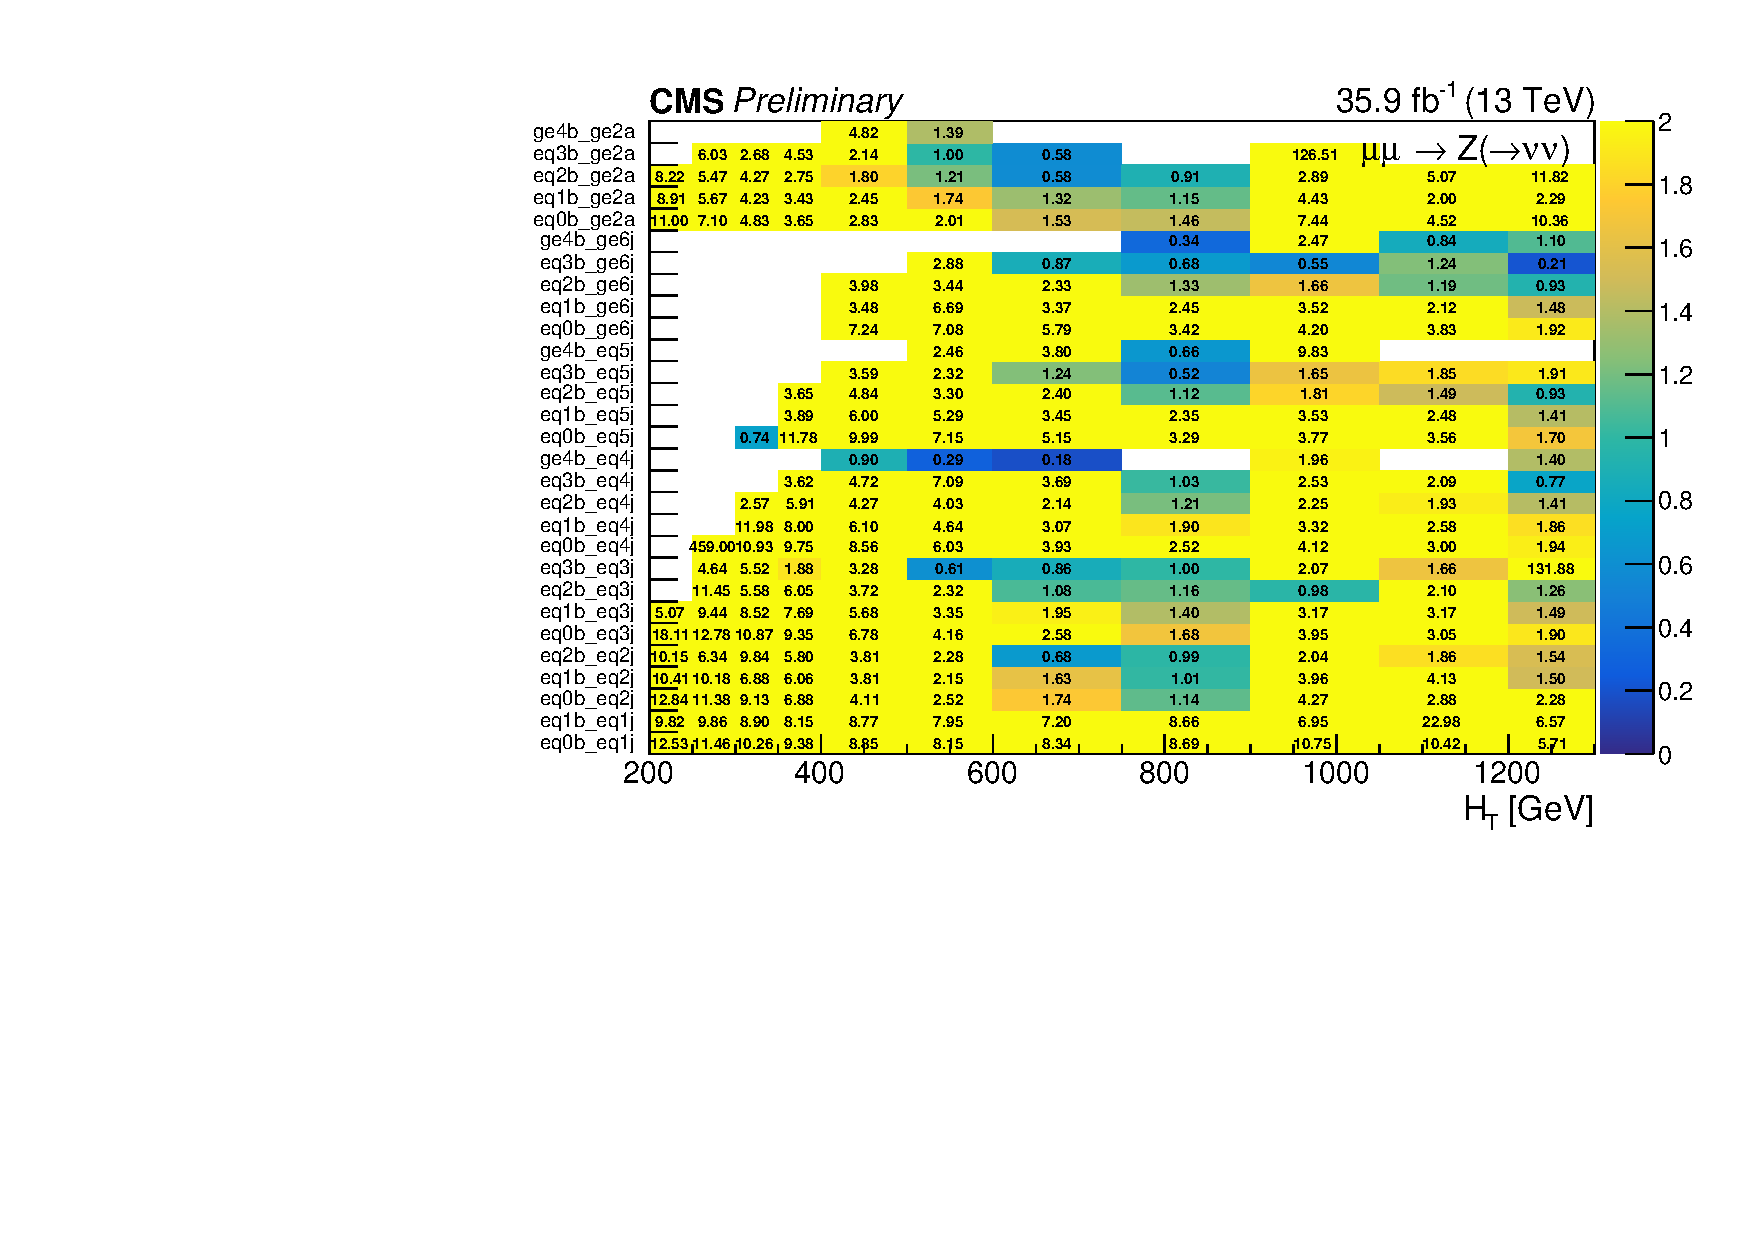
\includegraphics[width=0.5\textwidth]{figures/mcSystematics36p4fb/plots/tf_mumu_Zinv_2d_nominalUp.pdf}
  } \\
  \subfigure[Transfer factor as a function of \njet.]{
    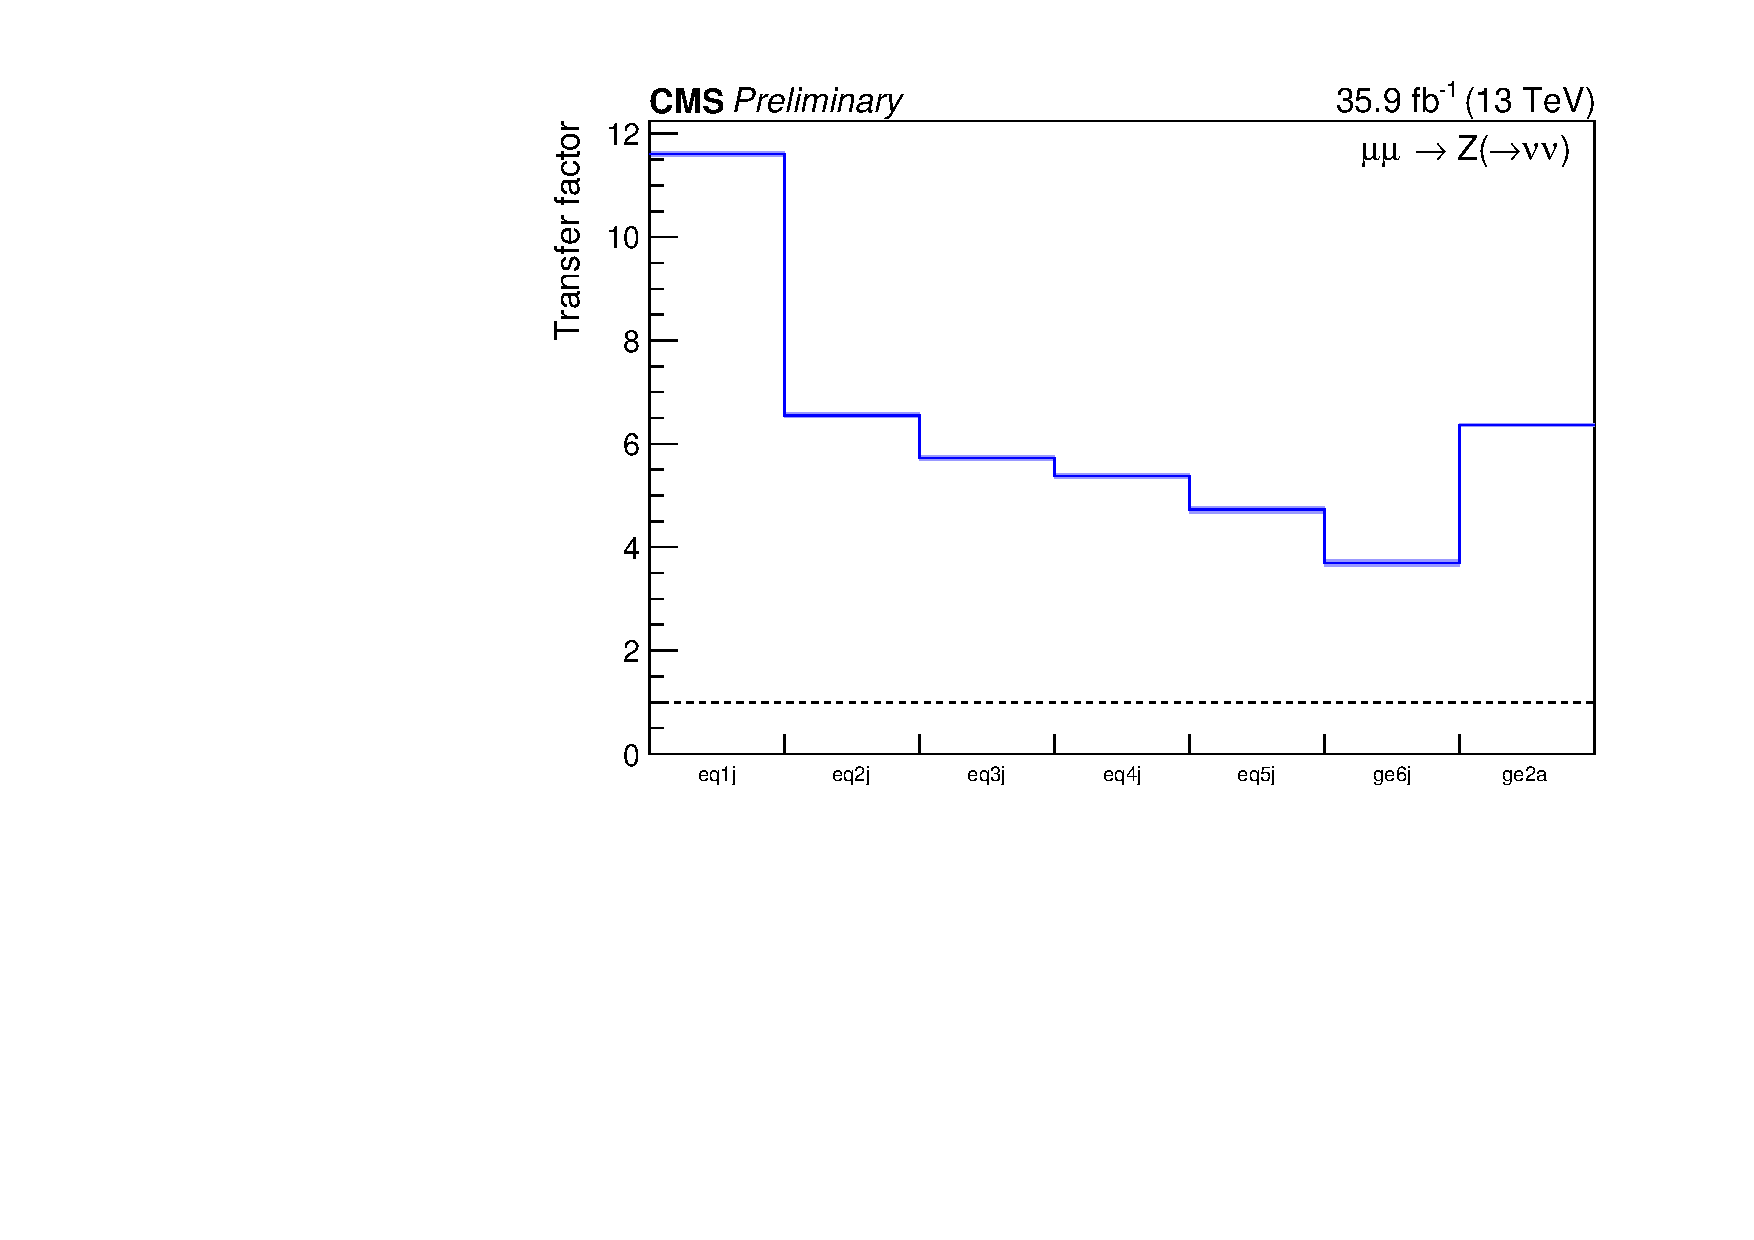
\includegraphics[width=0.5\textwidth]{figures/mcSystematics36p4fb/plots/tf_mumu_Zinv_njet_nominalUp.pdf}
  } ~
  \subfigure[Transfer factor as a function of \scalht.]{
    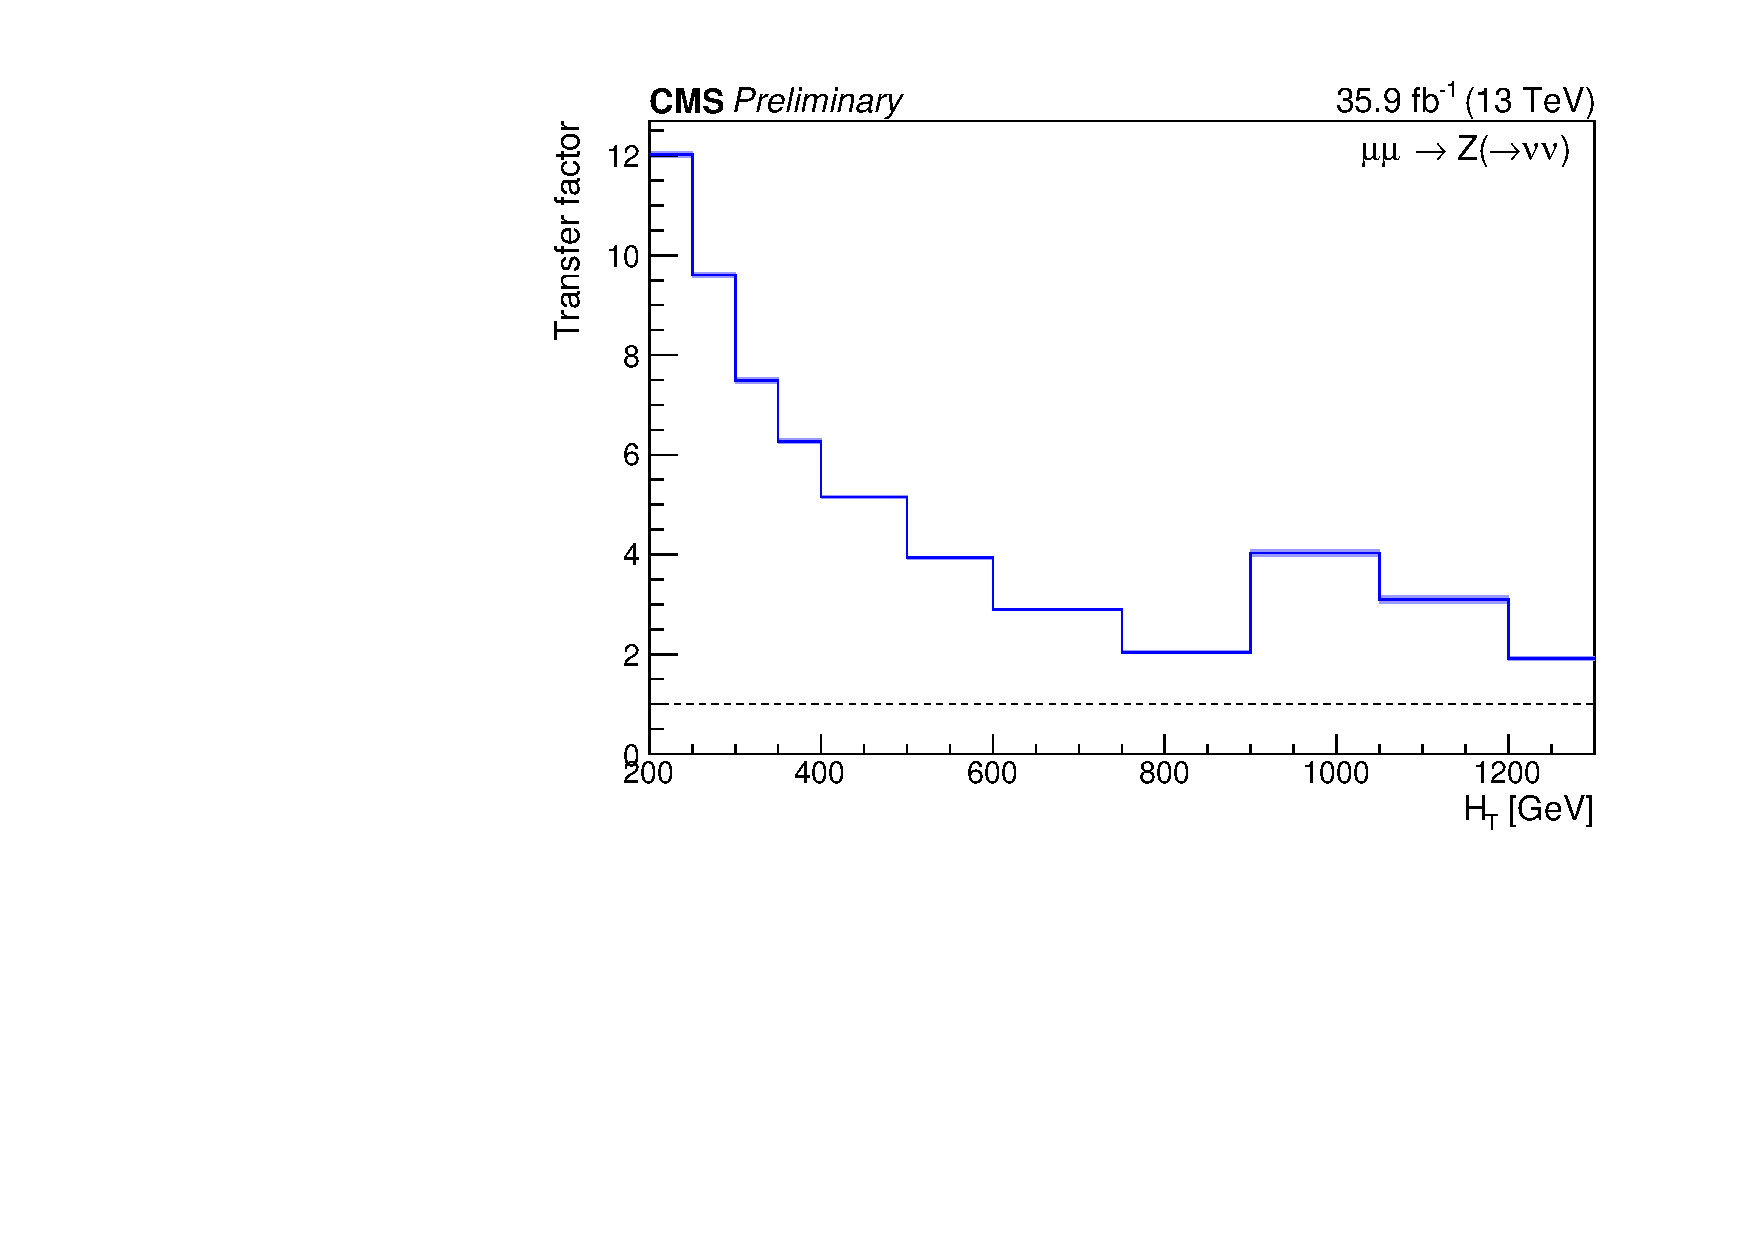
\includegraphics[width=0.5\textwidth]{figures/mcSystematics36p4fb/plots/tf_mumu_Zinv_ht_nominalUp.pdf}
  } \\
  \subfigure[Transfer factor as a function of \nb.]{
    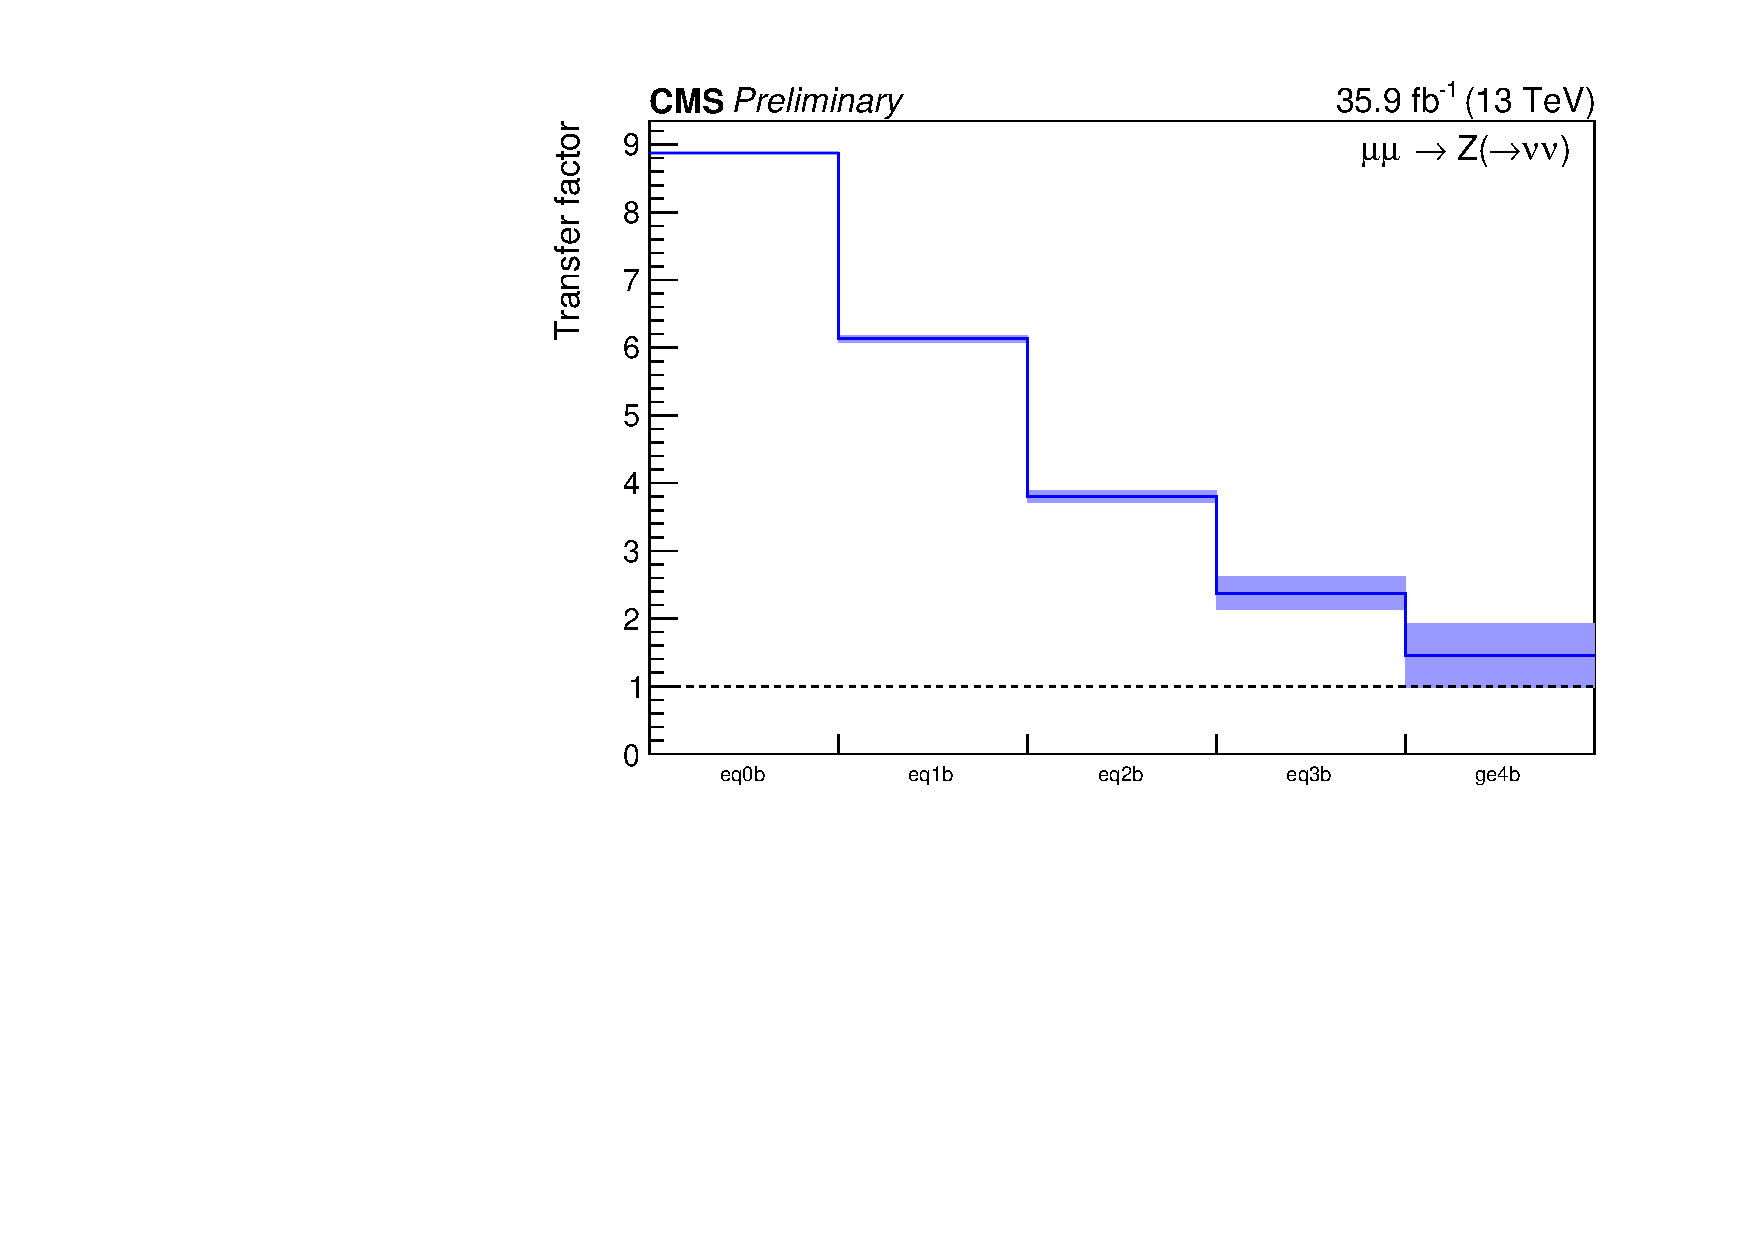
\includegraphics[width=0.5\textwidth]{figures/mcSystematics36p4fb/plots/tf_mumu_Zinv_bjet_nominalUp.pdf}
  } ~
  \subfigure[Transfer factor as a function of \mht.]{
    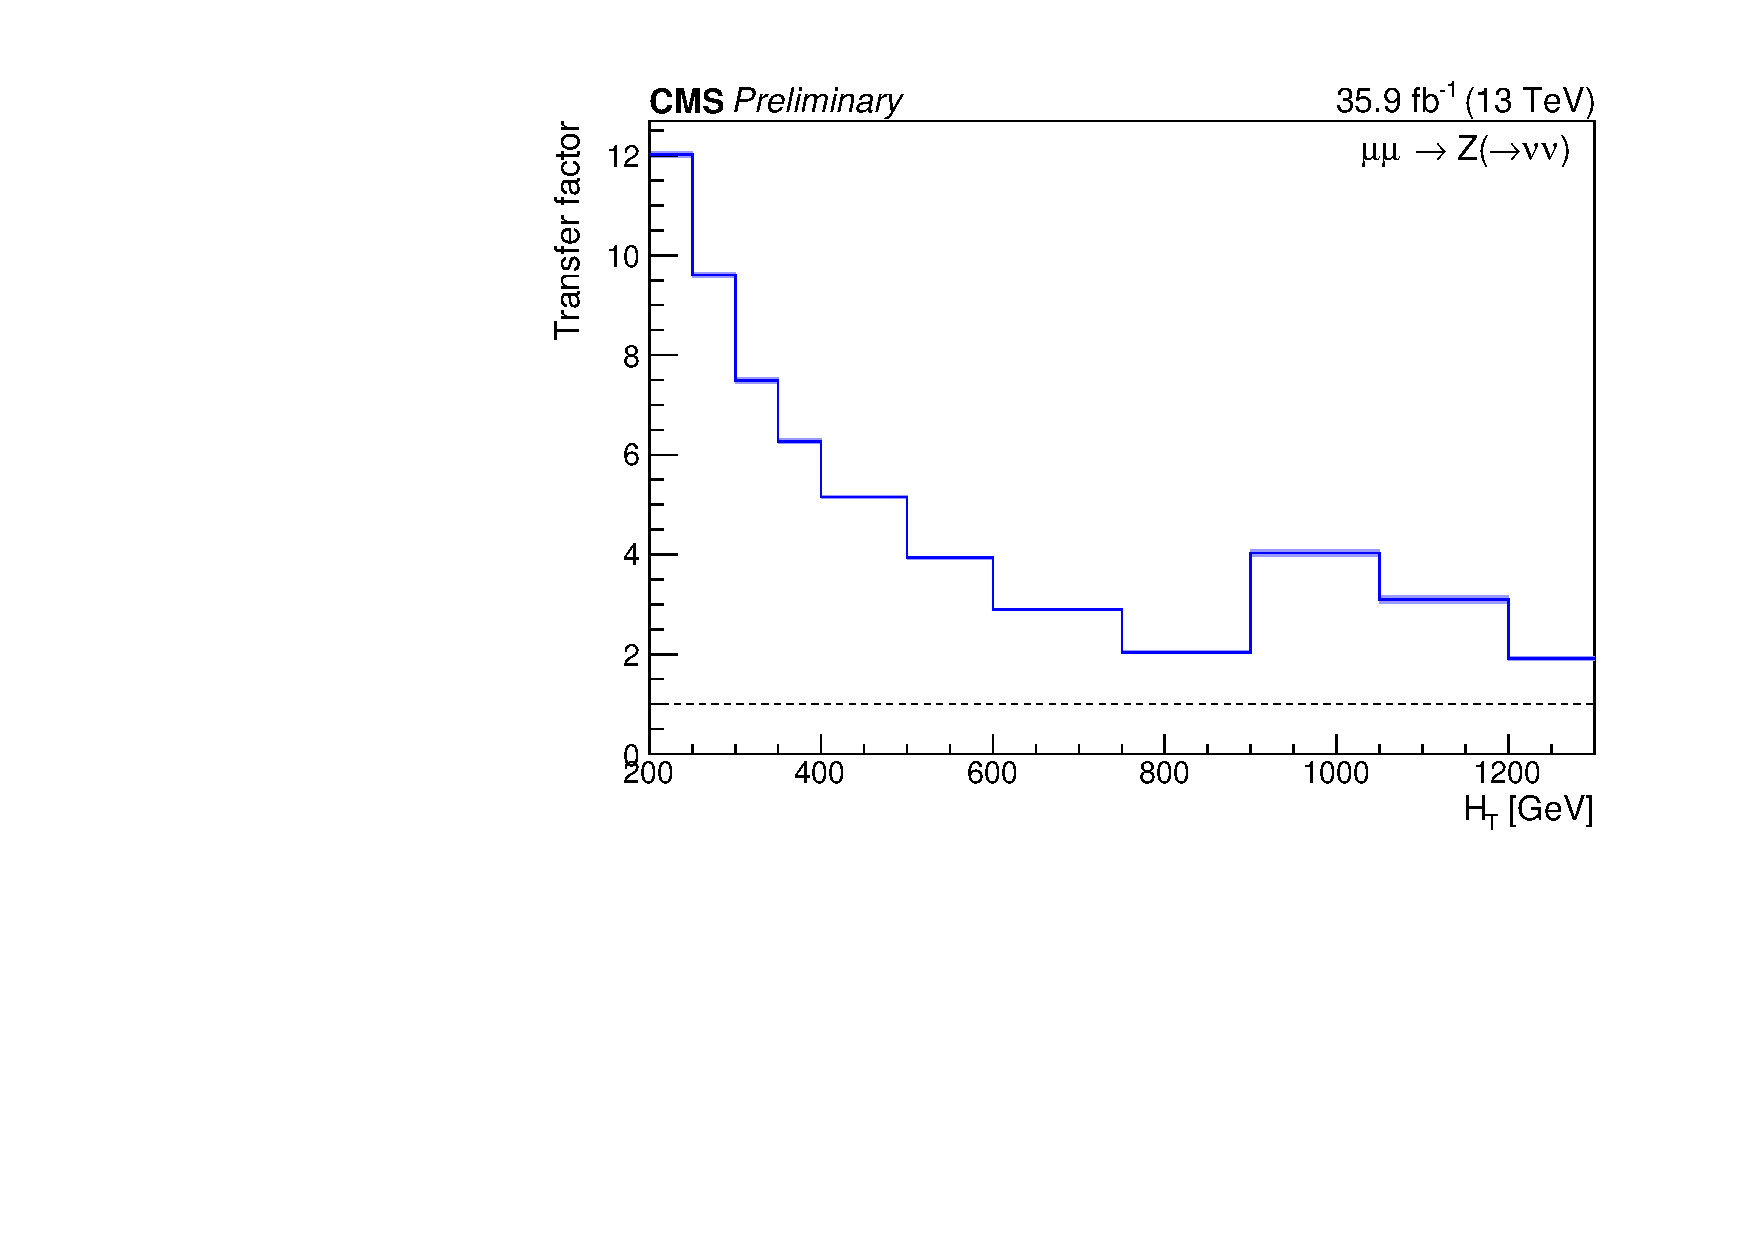
\includegraphics[width=0.5\textwidth]{figures/mcSystematics36p4fb/plots/tf_mumu_Zinv_ht_nominalUp.pdf}
  } \\
  \caption{\label{fig:tf_mumuToZinv} Transfer factors as a function of
    (\njet, \nb) event category and \scalht. Also shown are
    ``inclusive'' transfer factors as a function of \njet, \scalht,
    \nb, and \HTmiss. (Each ``inclusive'' dependence is shown when
    integrating over all other variables.) }
\end{figure}

\clearpage
\subsection{Minimum bias cross section / pileup}

\begin{figure}[!h]
  \centering
  \subfigure[Up variation versus (\njet,\nb) category and \scalht.]{
    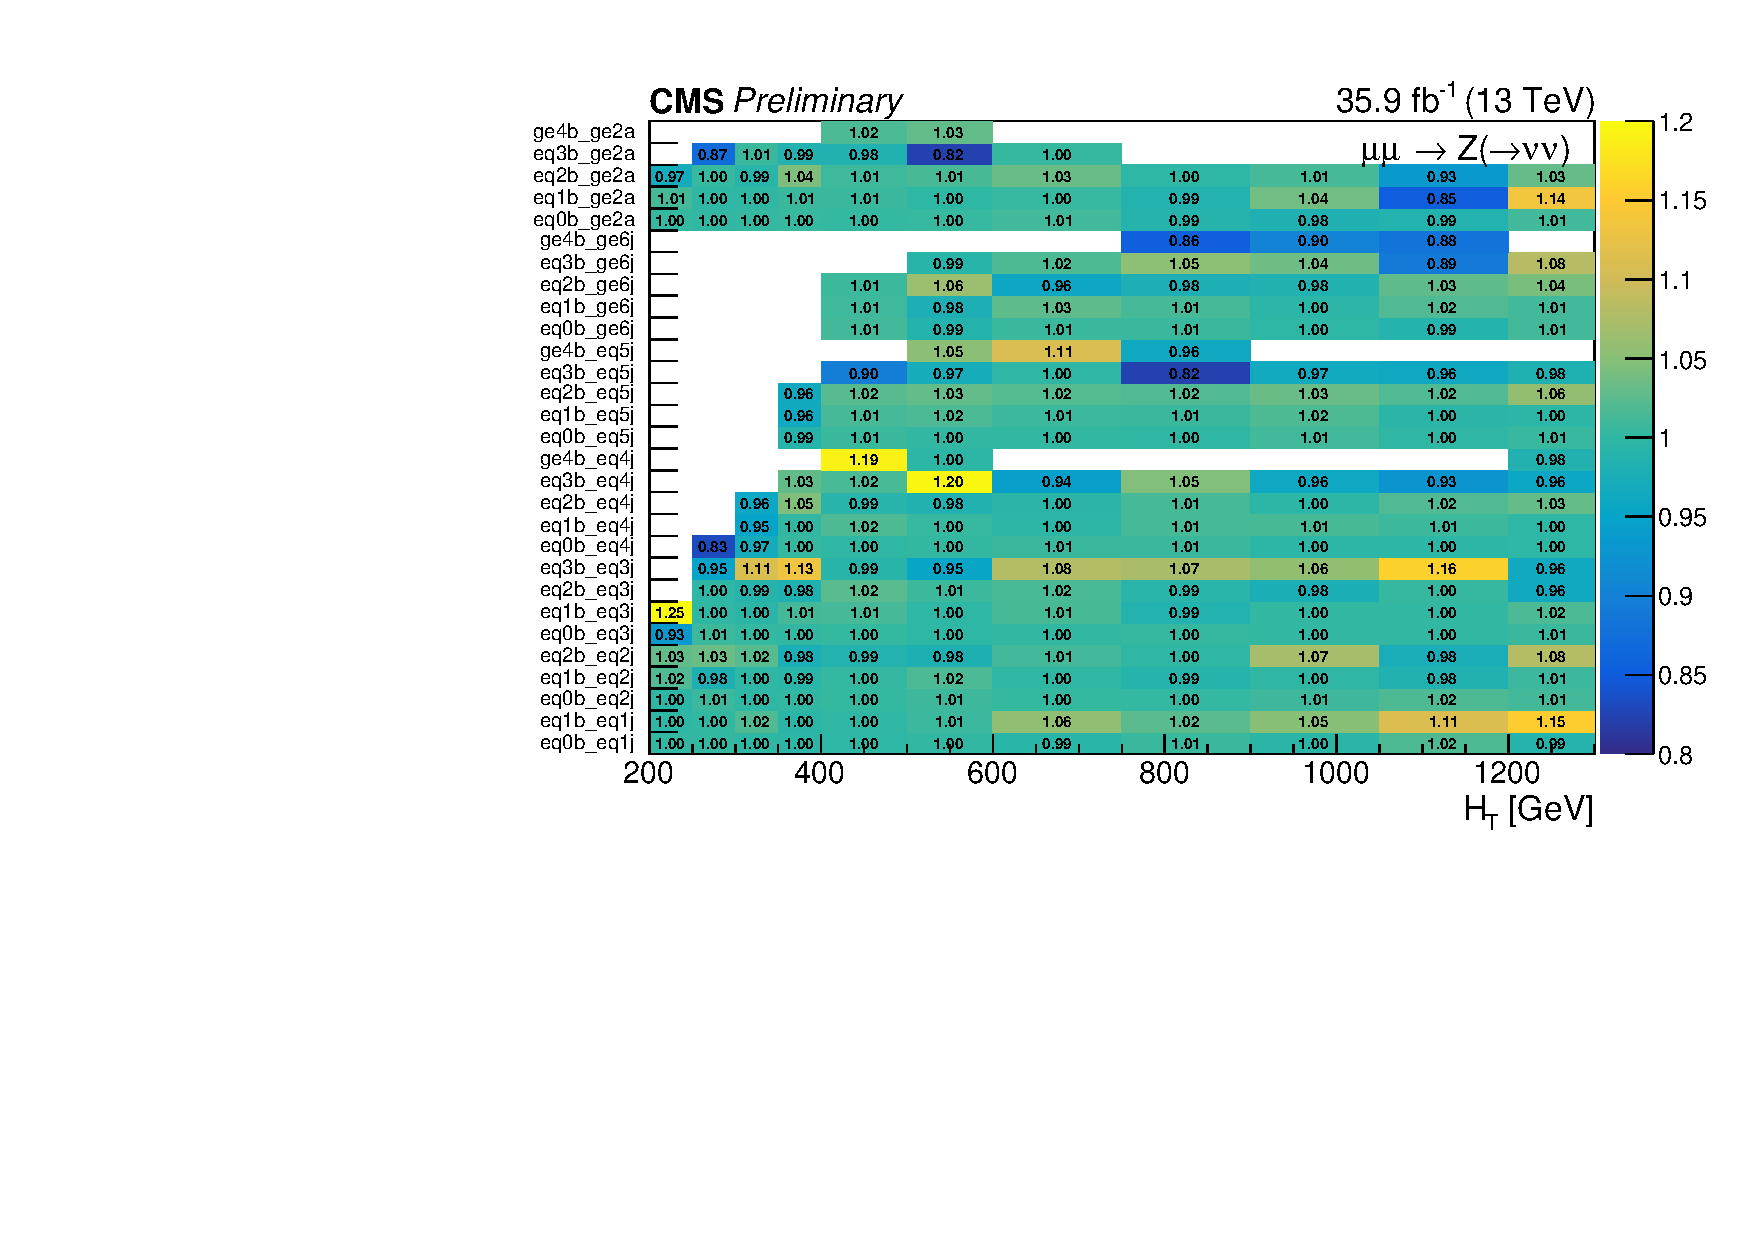
\includegraphics[width=0.5\textwidth]{figures/mcSystematics36p4fb/plots/tfratio_mumu_Zinv_2d_puWeightUp.pdf}
  } ~
  \subfigure[Down variation versus (\njet,\nb) category and \scalht.]{
    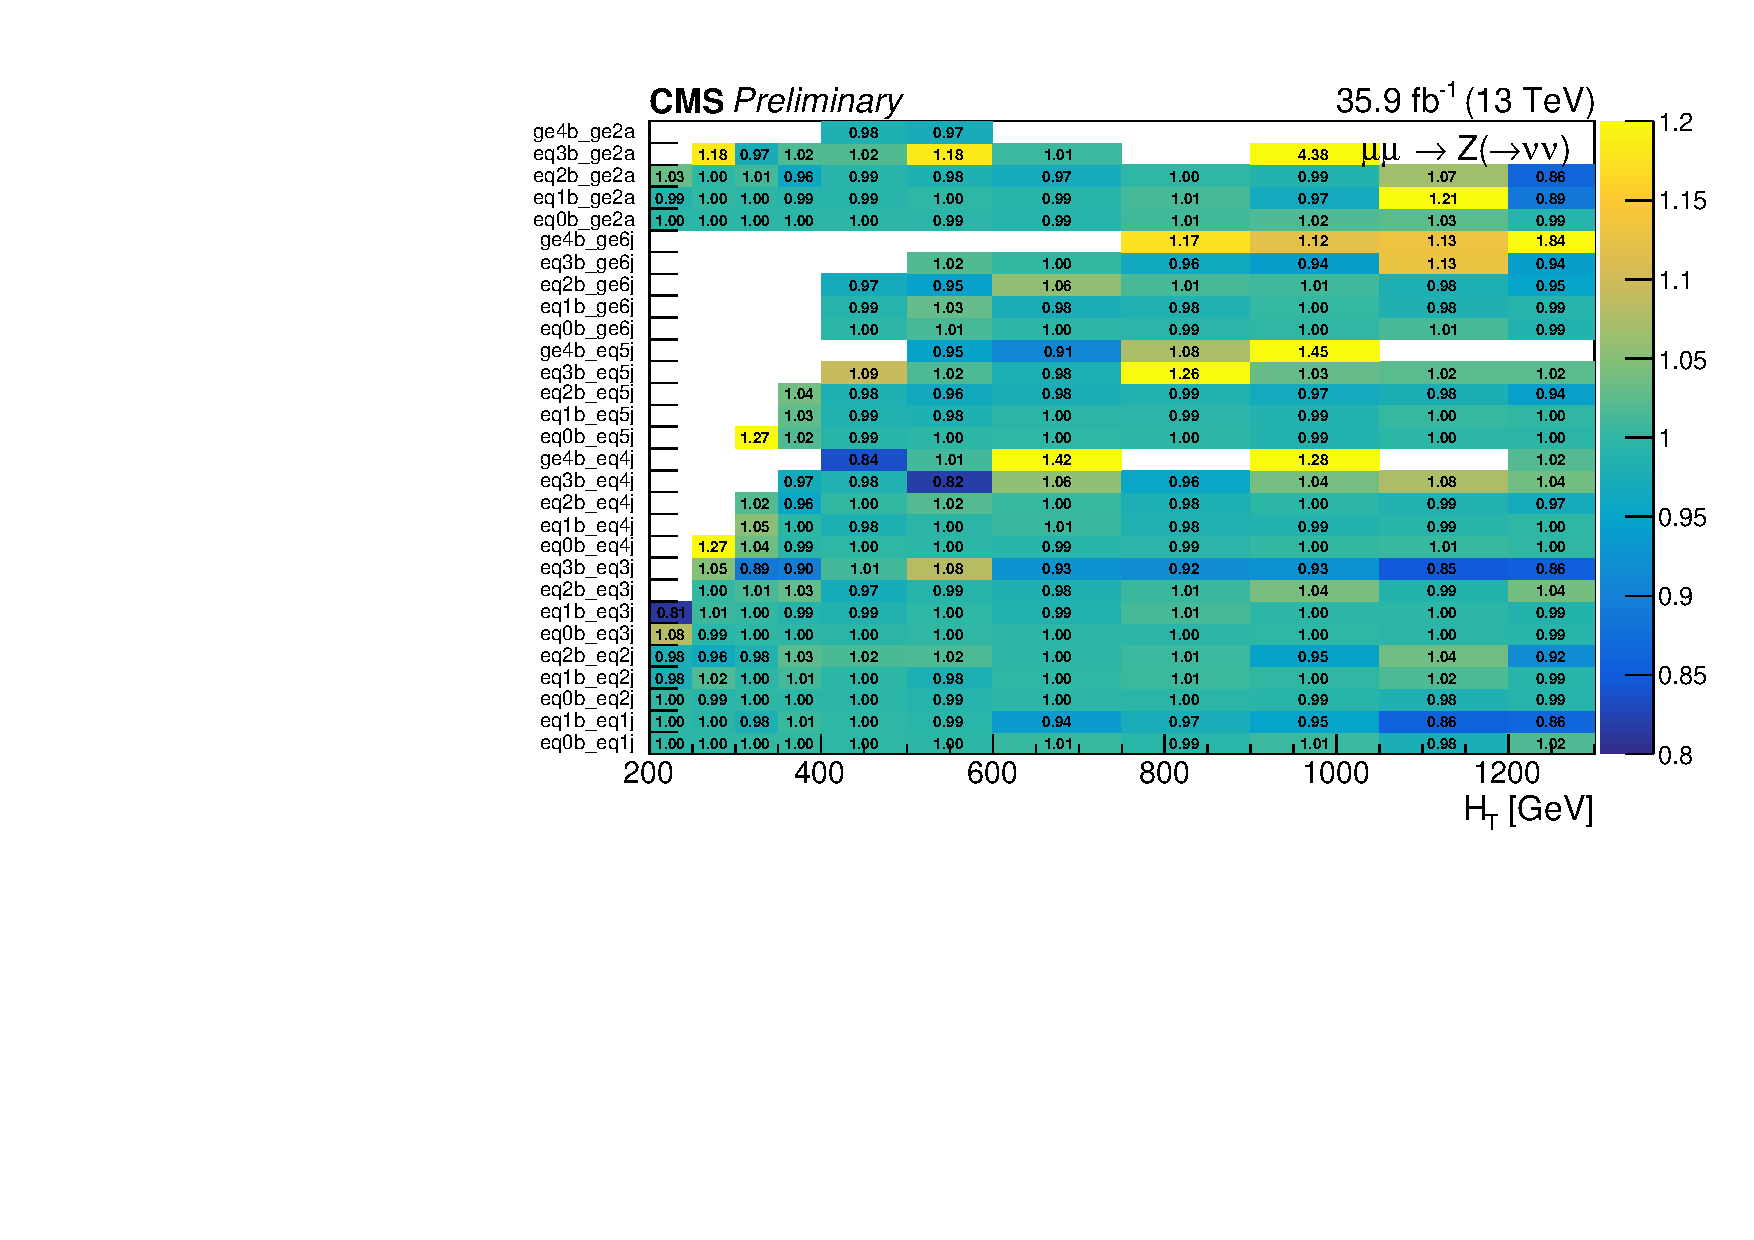
\includegraphics[width=0.5\textwidth]{figures/mcSystematics36p4fb/plots/tfratio_mumu_Zinv_2d_puWeightDown.pdf}
  }\\
  \subfigure[Up/down variations versus \njet.]{
    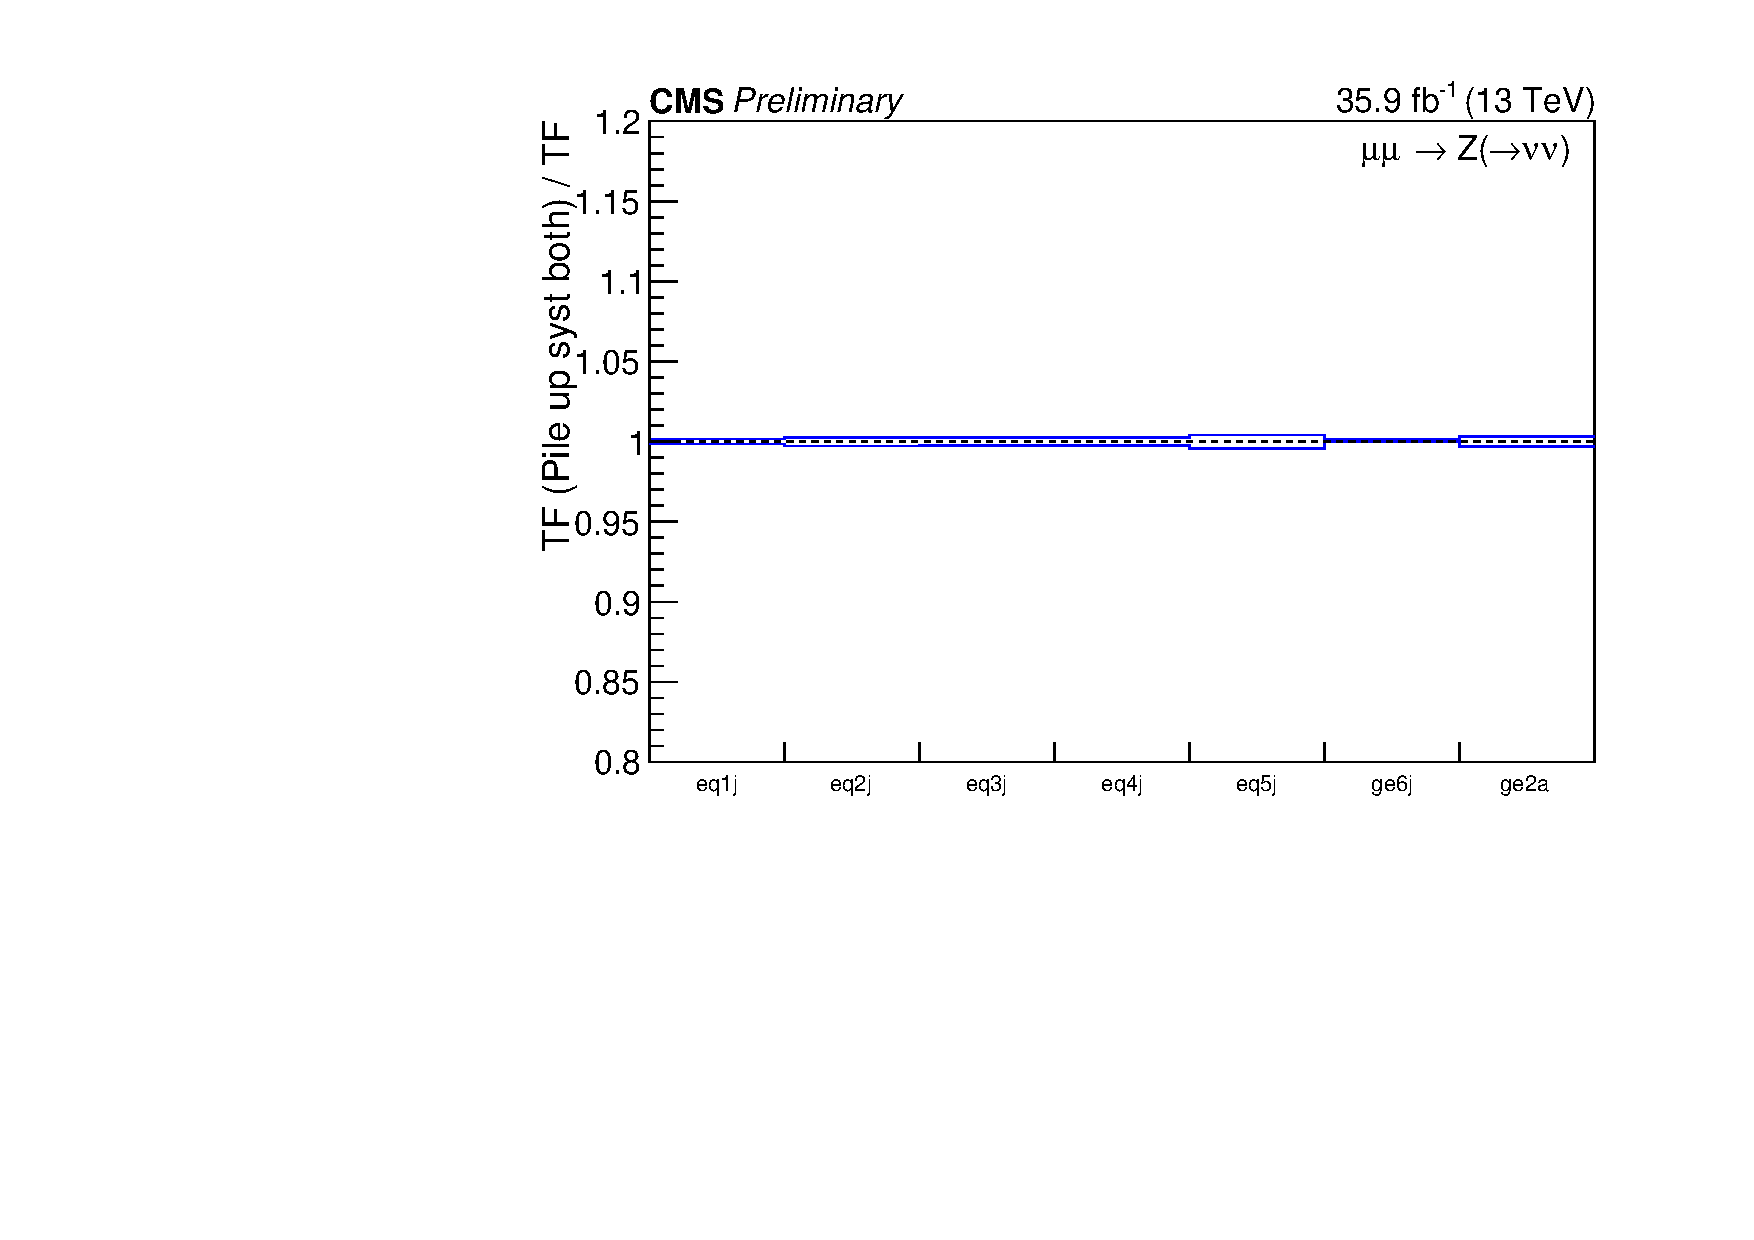
\includegraphics[width=0.5\textwidth]{figures/mcSystematics36p4fb/plots/tfratio_mumu_Zinv_njet_puWeightUp.pdf}
  } ~
  \subfigure[Up/down variations versus \scalht.]{
    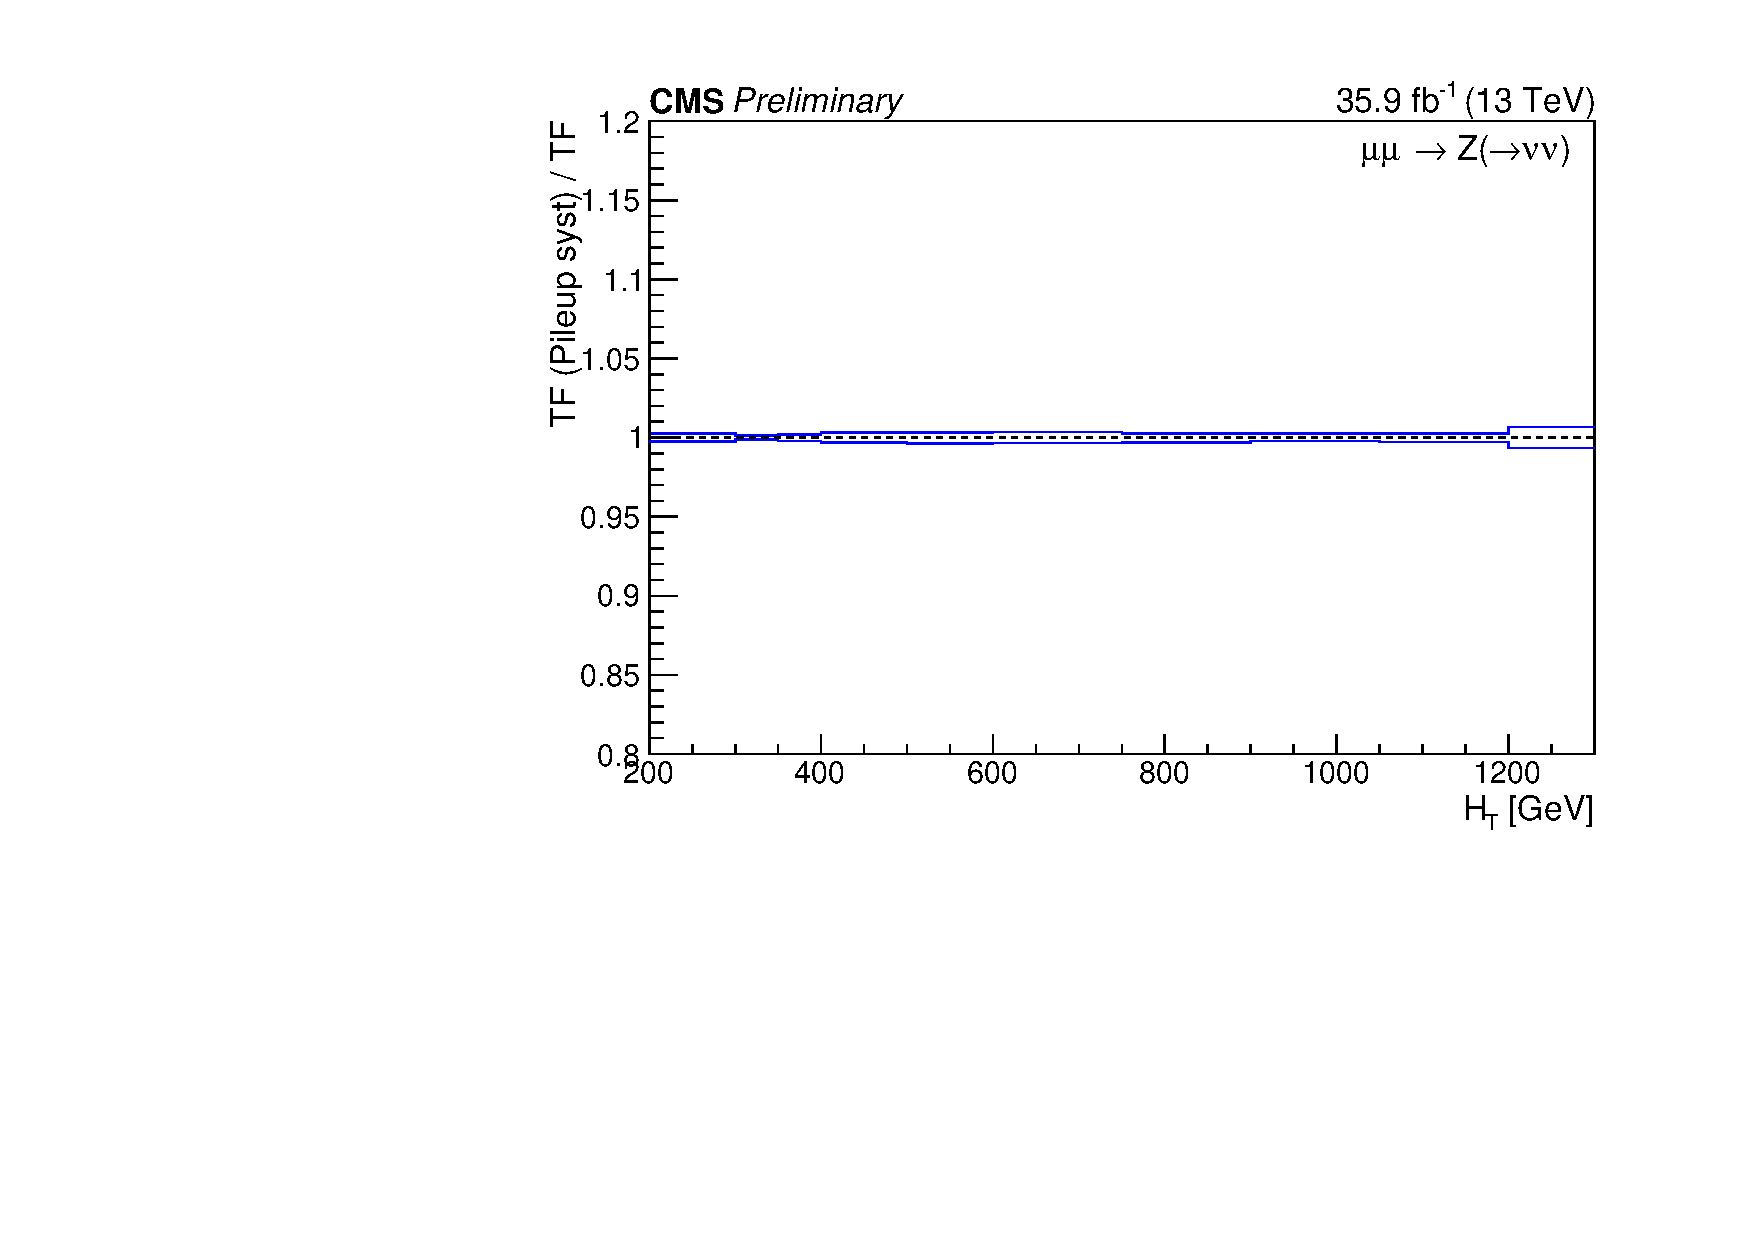
\includegraphics[width=0.5\textwidth]{figures/mcSystematics36p4fb/plots/tfratio_mumu_Zinv_ht_puWeightUp.pdf}
  } \\
  \subfigure[Up/down variations versus \nb.]{
    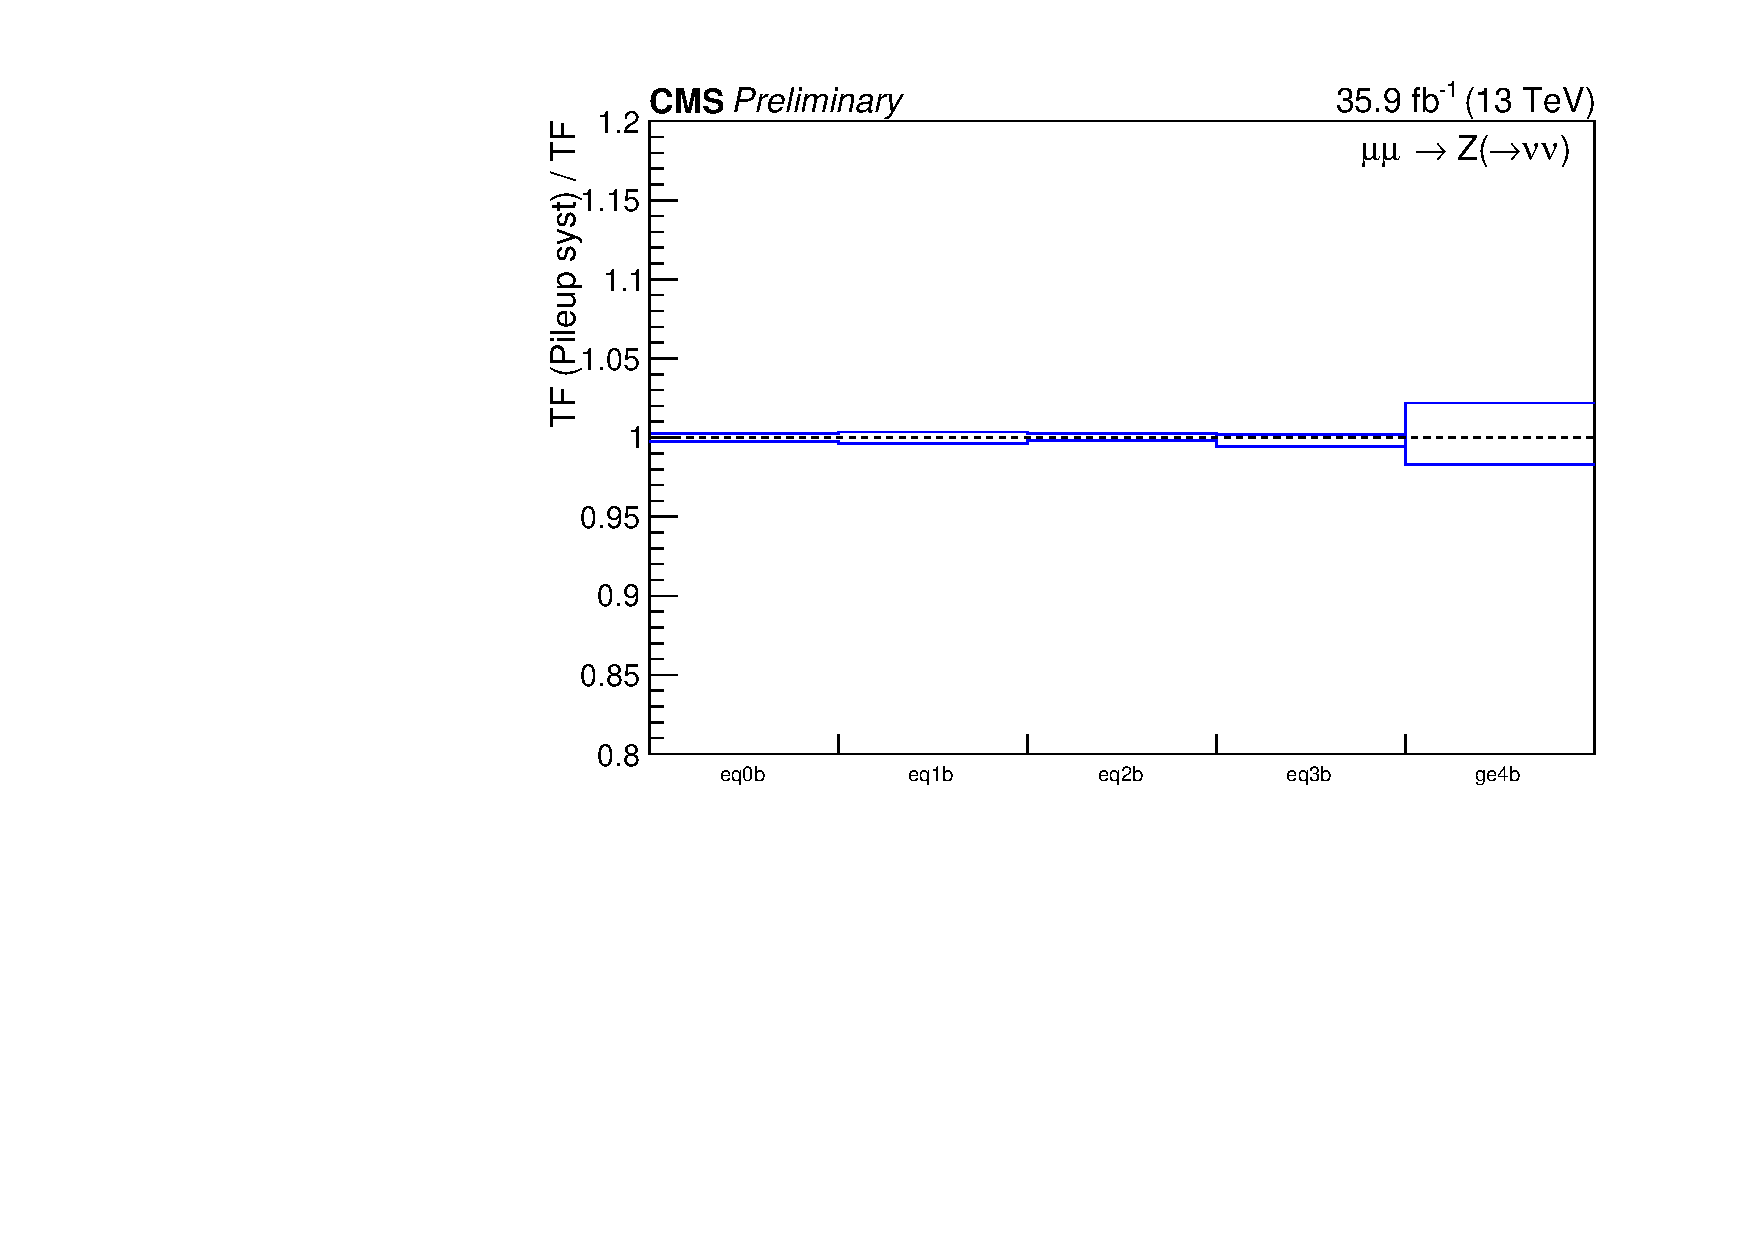
\includegraphics[width=0.5\textwidth]{figures/mcSystematics36p4fb/plots/tfratio_mumu_Zinv_bjet_puWeightUp.pdf}
  } ~
  \subfigure[Up/down variations versus \mht.]{
    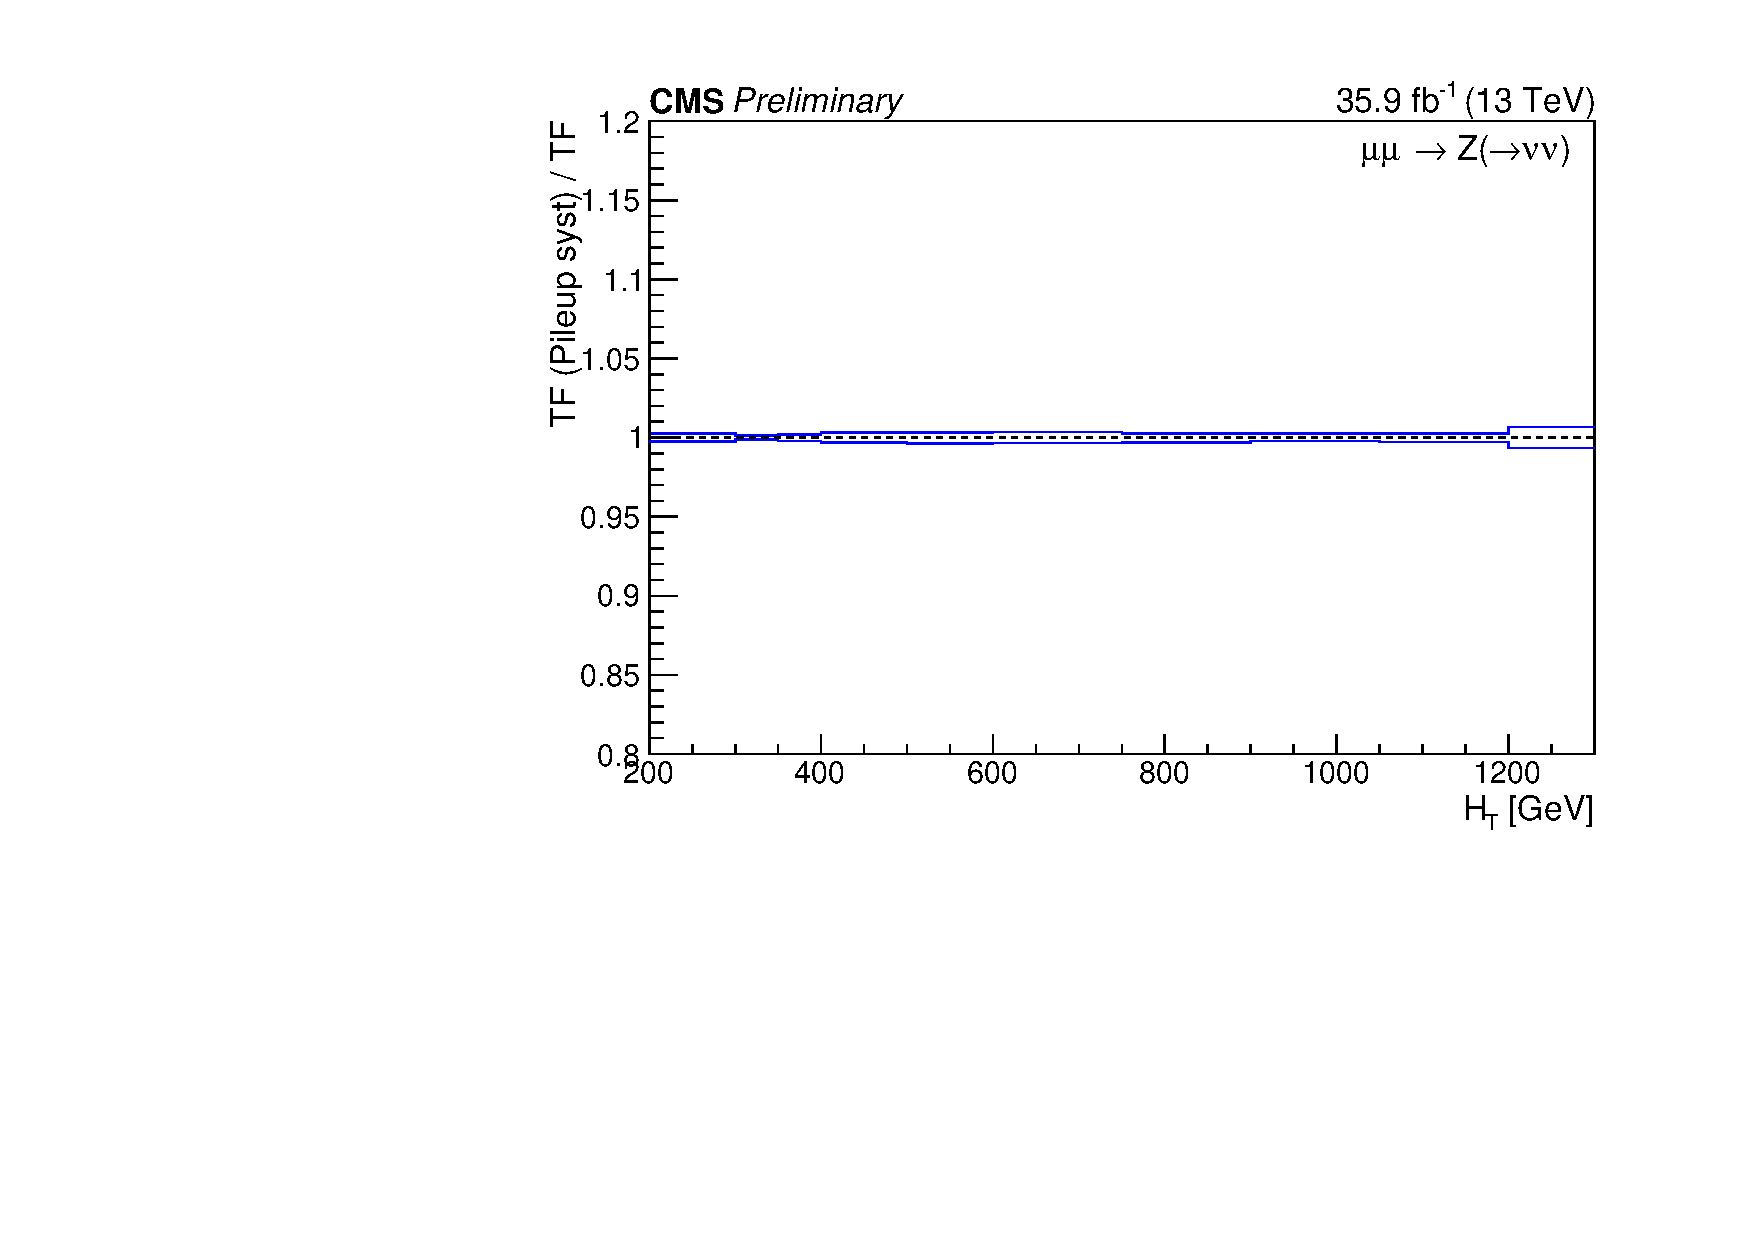
\includegraphics[width=0.5\textwidth]{figures/mcSystematics36p4fb/plots/tfratio_mumu_Zinv_ht_puWeightUp.pdf}
  } \\
  \caption{\label{fig:tfSyst_pu_mumuToZinv} The relative change in the
    ``$\mmj \rightarrow \znunu\ + \textrm{jets}$'' transfer factors from
    simulation due to $\pm1\sigma$ uncertainties in pileup.  }
\end{figure}

\clearpage
\subsection{Effect of scale and PDF on lepton acceptance}

\begin{figure}[!h]
  \centering
  \subfigure[Up variation versus (\njet,\nb) category and \scalht.]{
    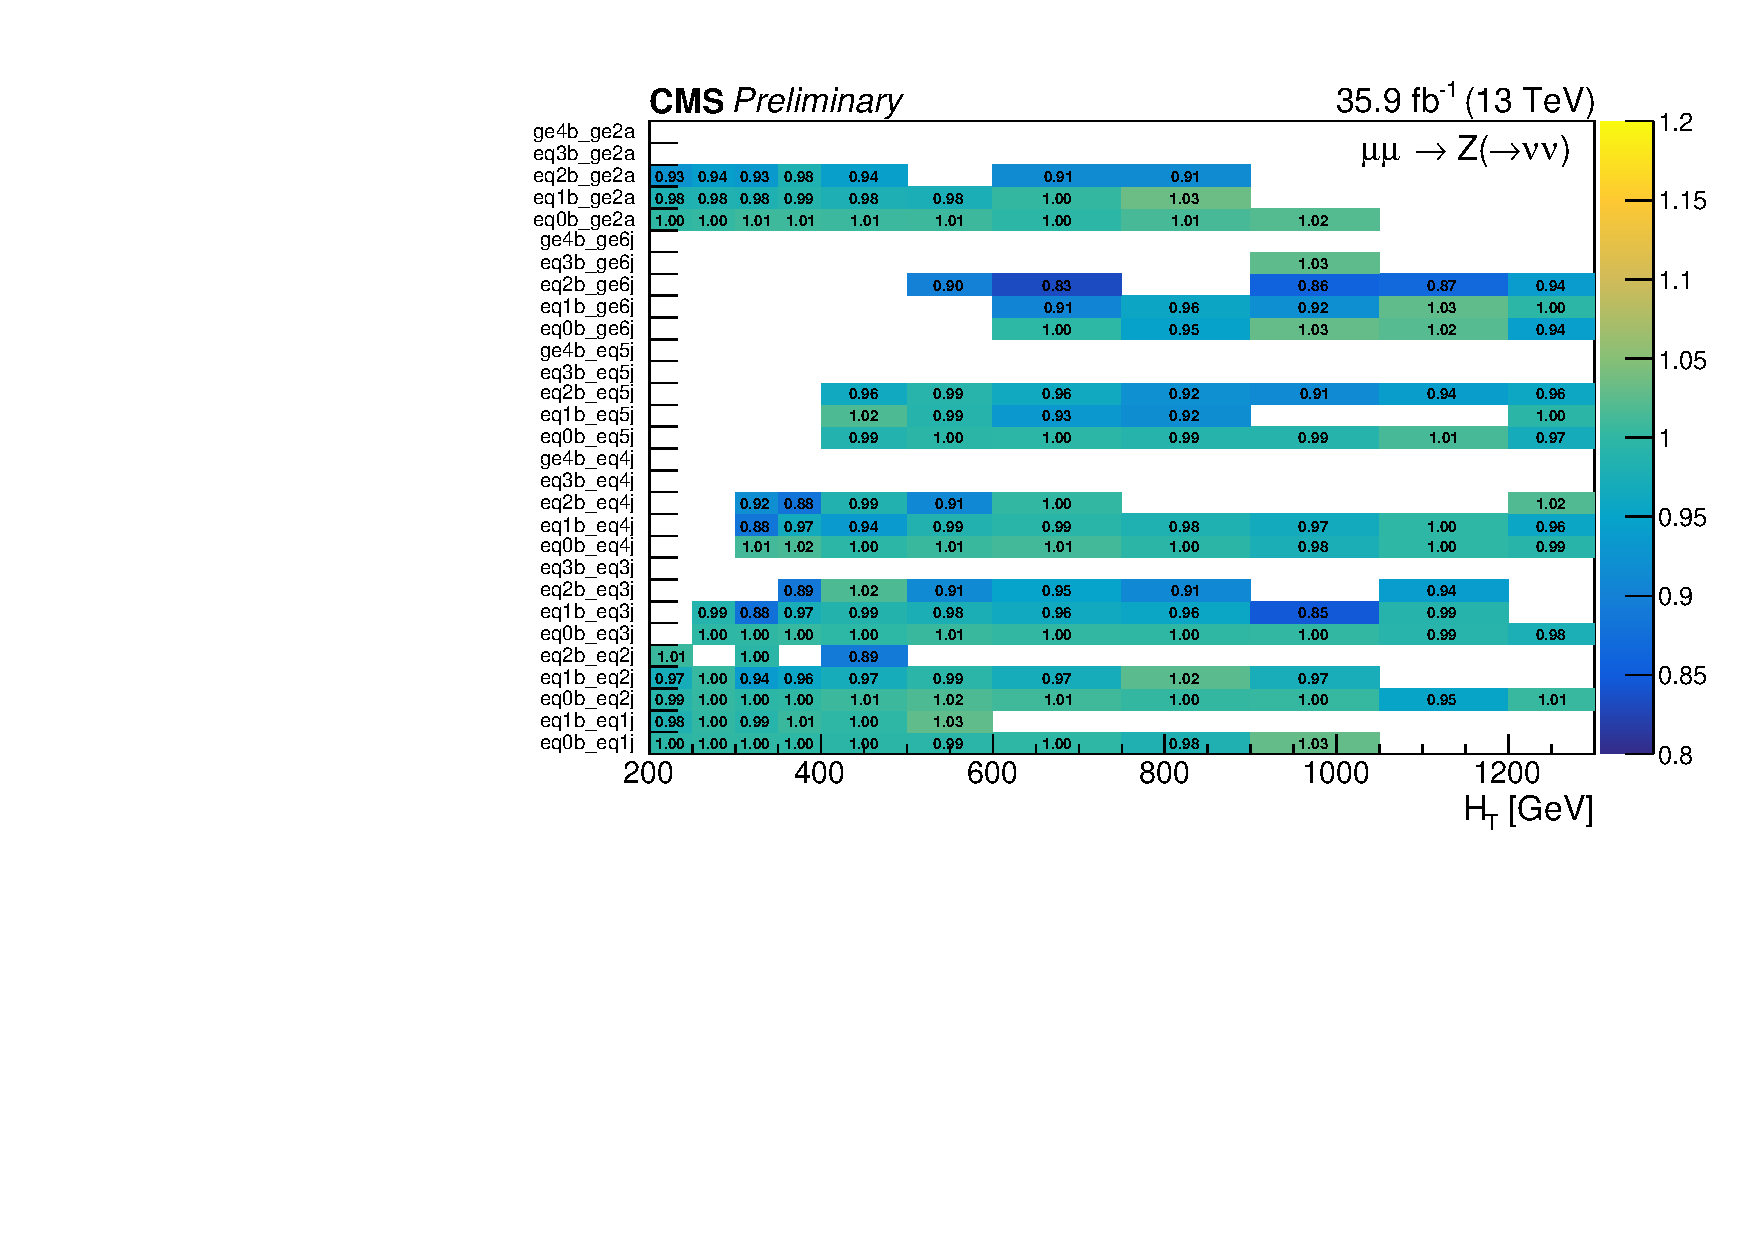
\includegraphics[width=0.5\textwidth]{figures/mcSystematics36p4fb/plots/tfratio_mumu_Zinv_2d_scaleWeightUp.pdf}
  } ~
  \subfigure[Down variation versus (\njet,\nb) category and \scalht.]{
    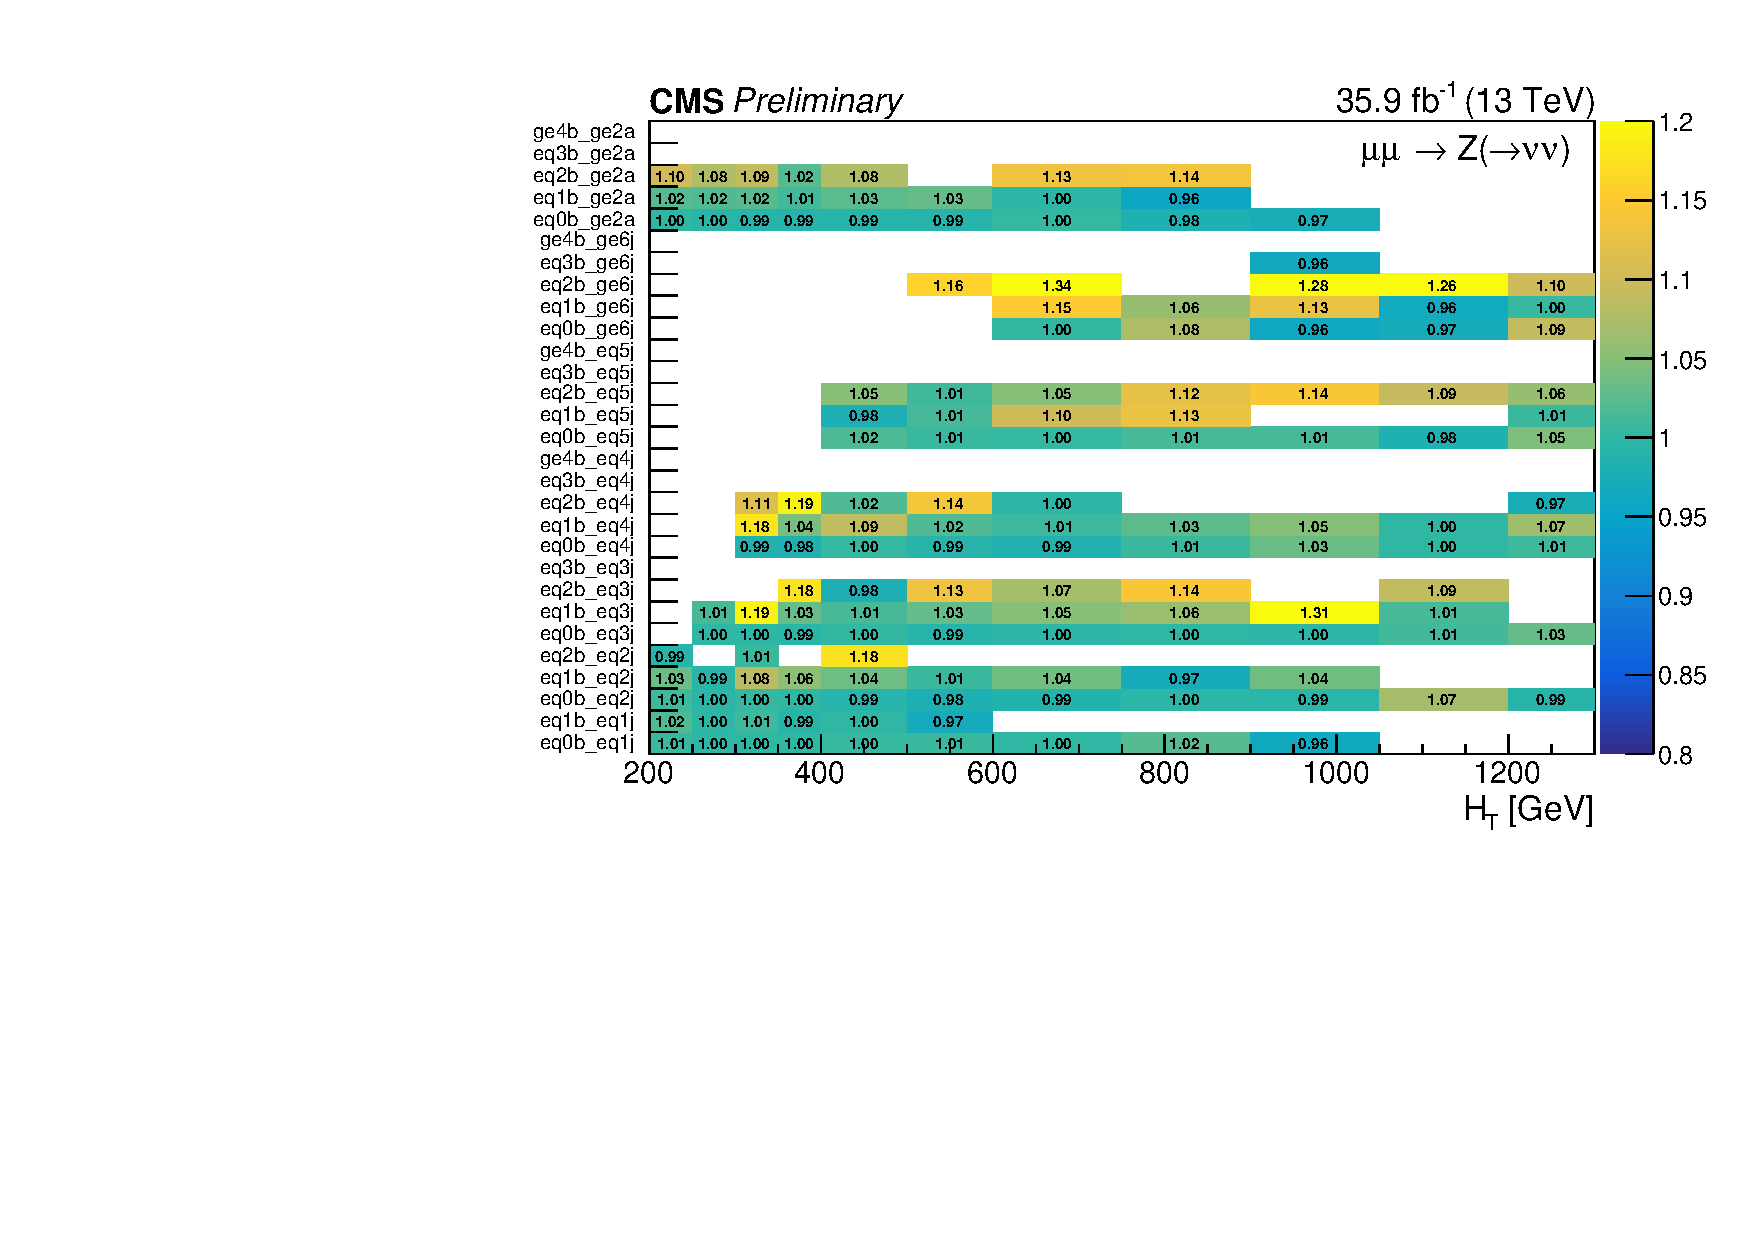
\includegraphics[width=0.5\textwidth]{figures/mcSystematics36p4fb/plots/tfratio_mumu_Zinv_2d_scaleWeightDown.pdf}
  }\\
  \subfigure[Up/down variations versus \njet.]{
    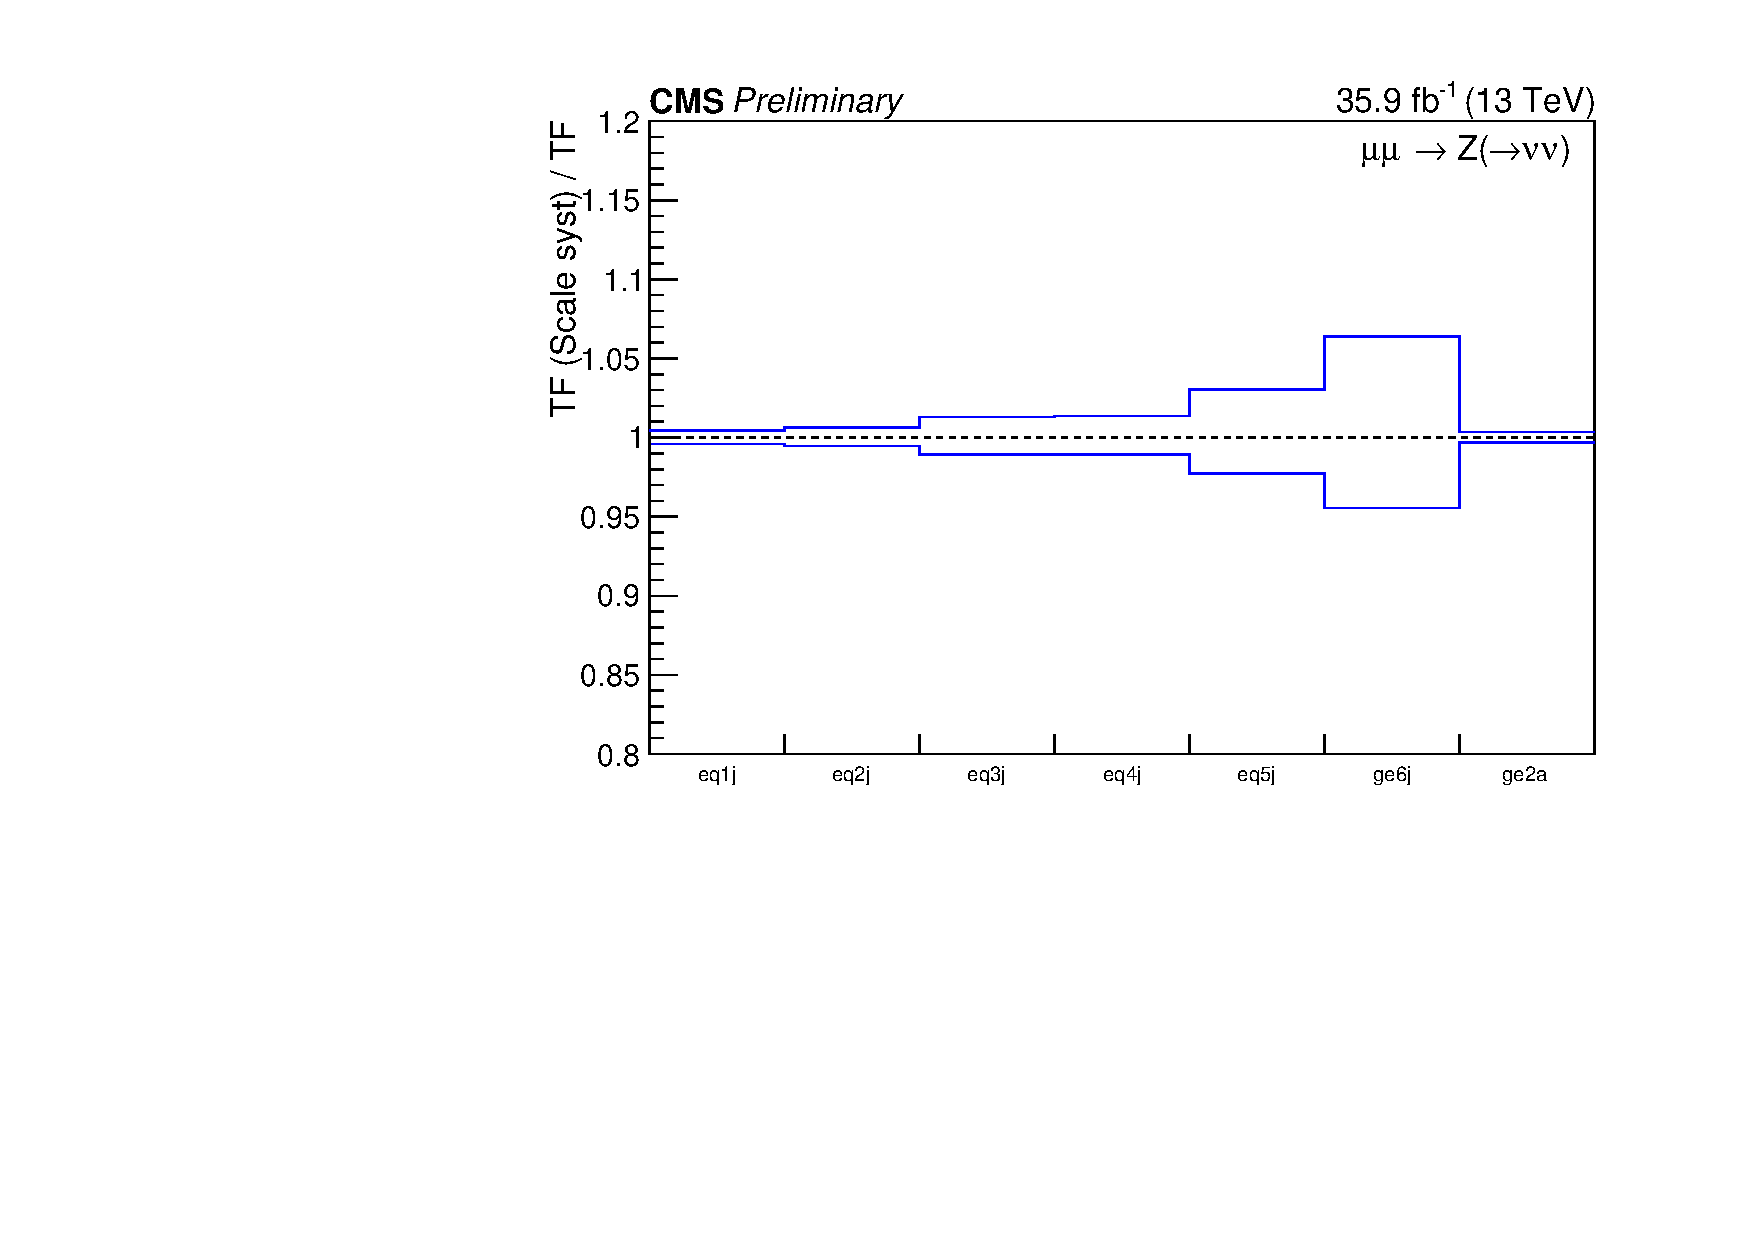
\includegraphics[width=0.5\textwidth]{figures/mcSystematics36p4fb/plots/tfratio_mumu_Zinv_njet_scaleWeightUp.pdf}
  } ~
  \subfigure[Up/down variations versus \scalht.]{
    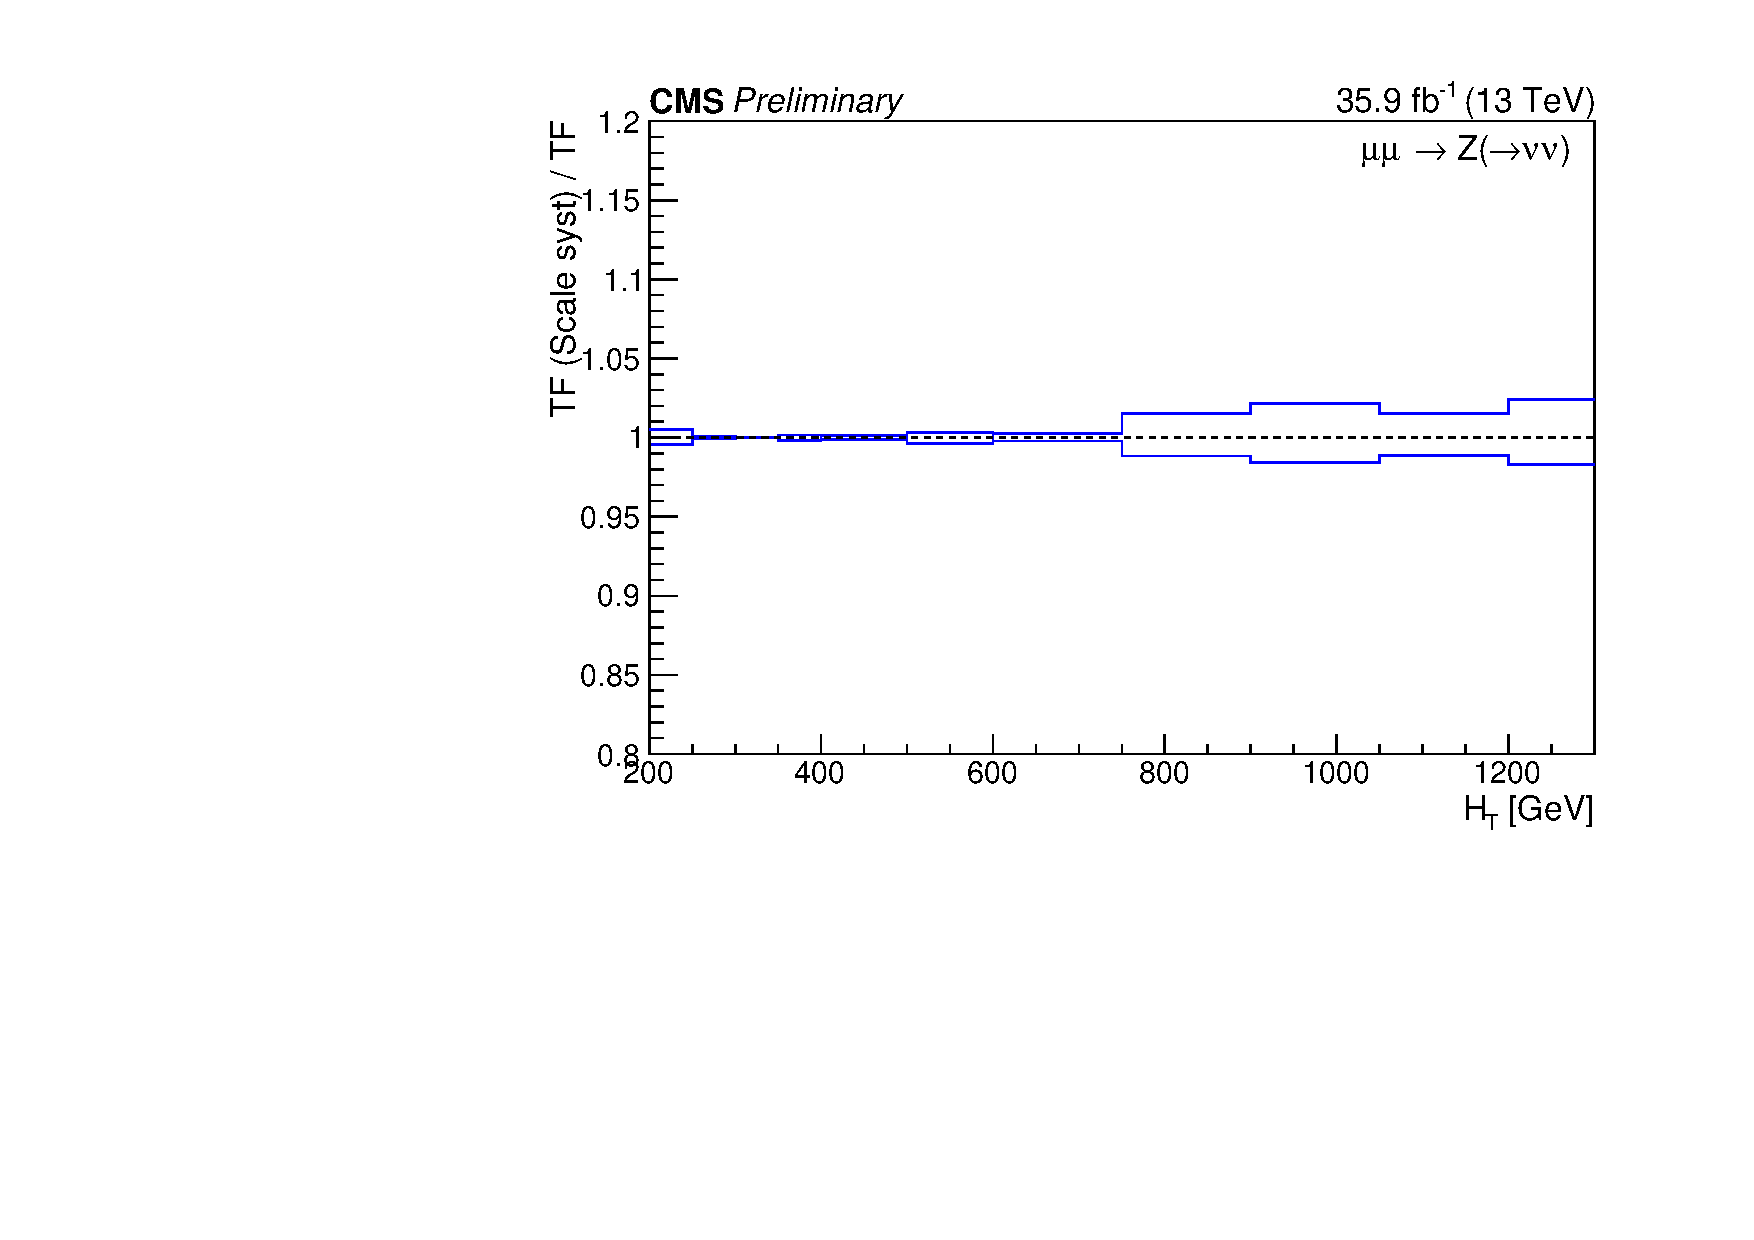
\includegraphics[width=0.5\textwidth]{figures/mcSystematics36p4fb/plots/tfratio_mumu_Zinv_ht_scaleWeightUp.pdf}
  } \\
  \subfigure[Up/down variations versus \nb.]{
    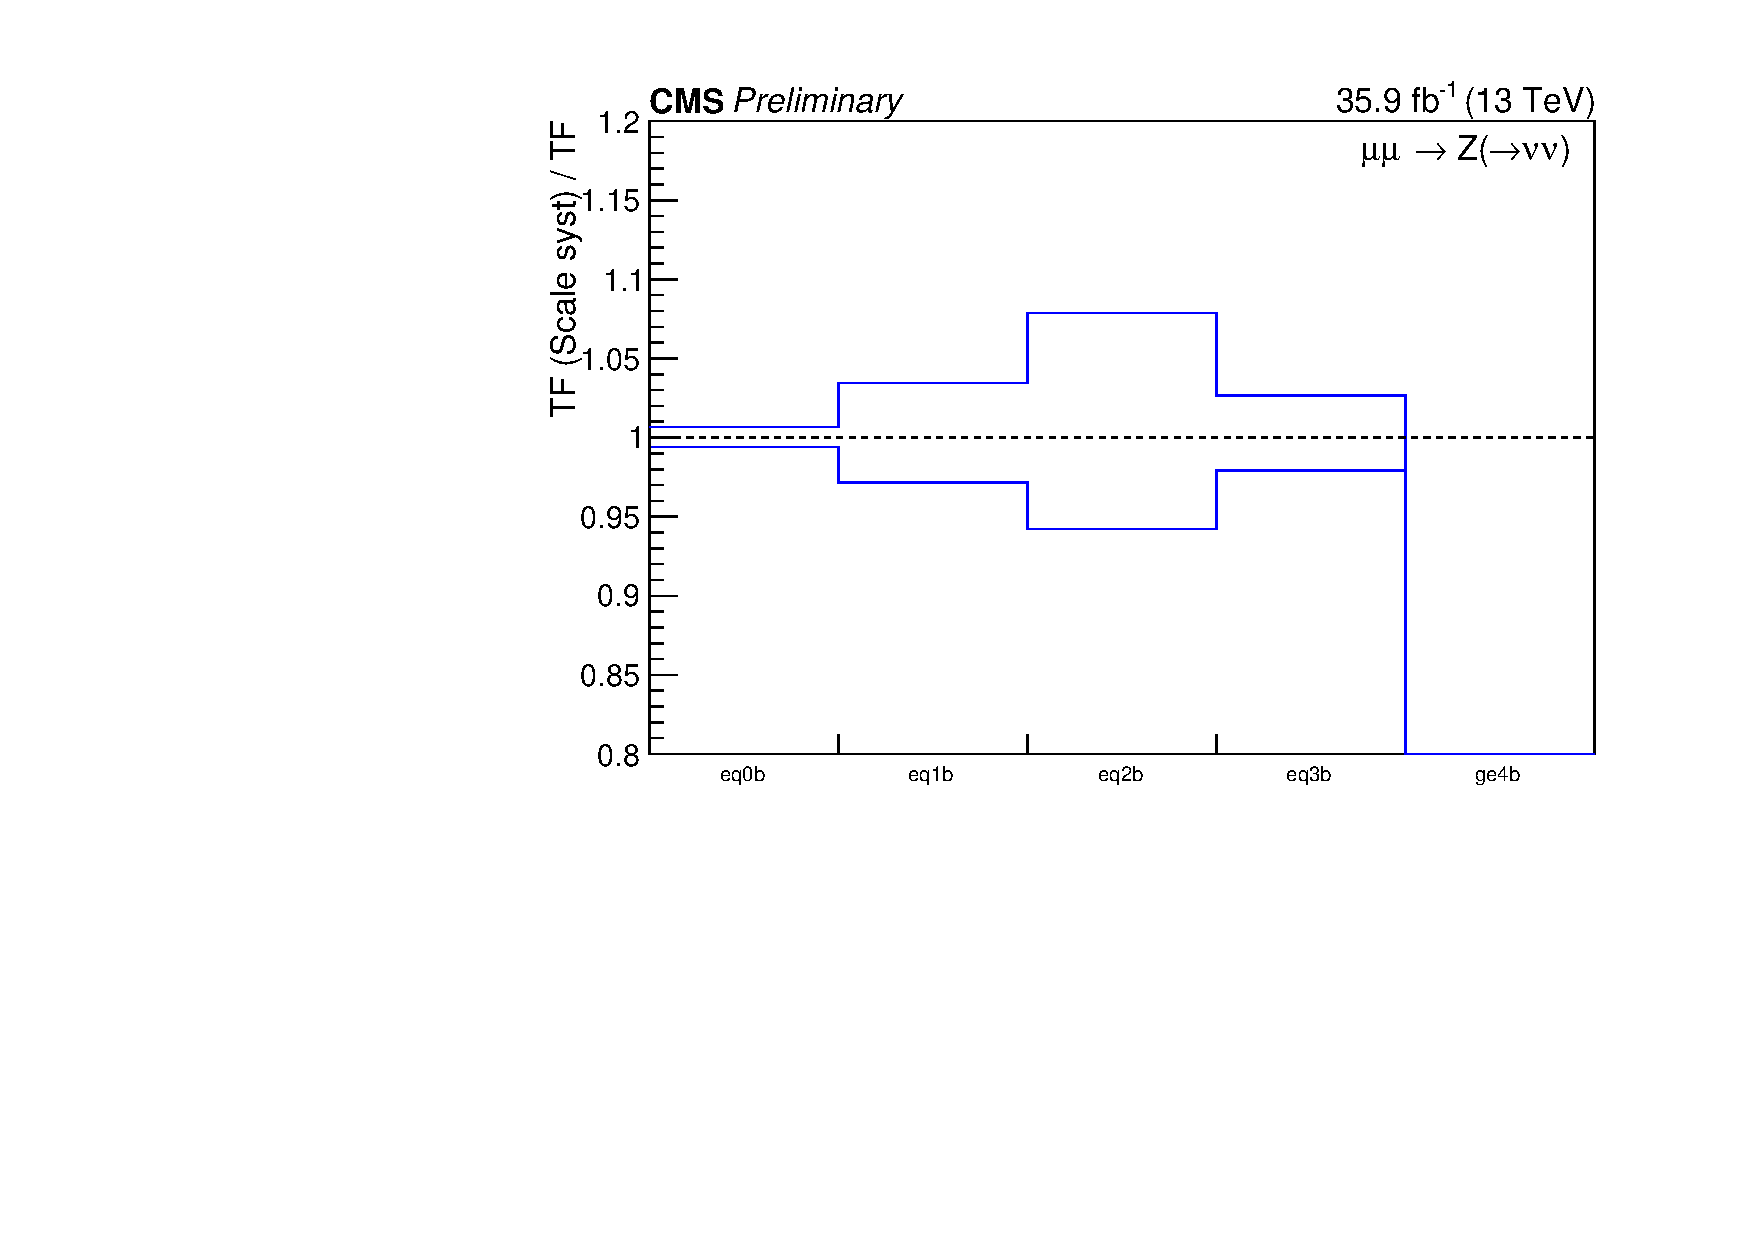
\includegraphics[width=0.5\textwidth]{figures/mcSystematics36p4fb/plots/tfratio_mumu_Zinv_bjet_scaleWeightUp.pdf}
  } ~
  \subfigure[Up/down variations versus \mht.]{
    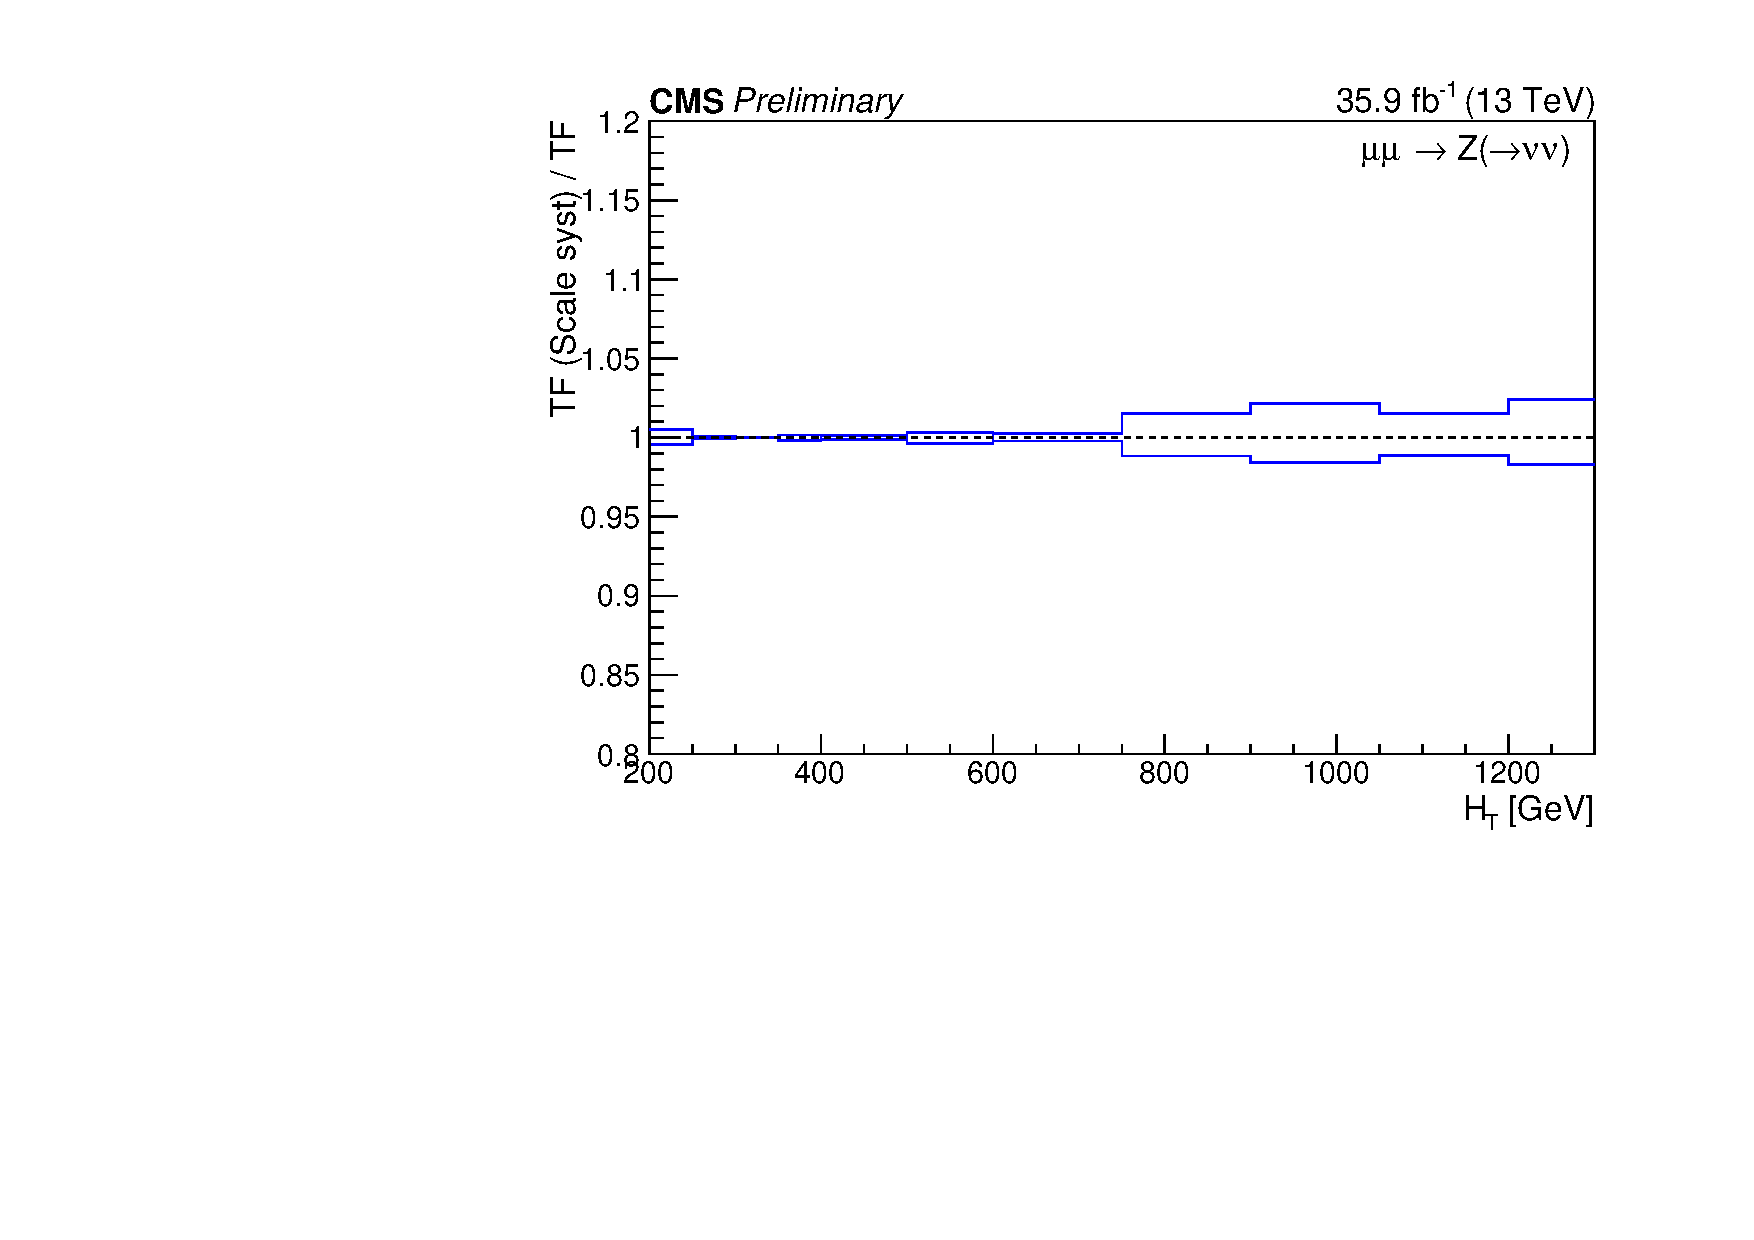
\includegraphics[width=0.5\textwidth]{figures/mcSystematics36p4fb/plots/tfratio_mumu_Zinv_ht_scaleWeightUp.pdf}
  } \\
  \caption{\label{fig:tfSyst_scale_mumuToZinv} The relative change in the
    ``$\mmj \rightarrow \znunu\ + \textrm{jets}$'' transfer factors from
    simulation due to $\pm1\sigma$ uncertainties in
    renormalisation/factorisation scales.  }
\end{figure}

\clearpage
\begin{figure}[!h]
  \centering
  \subfigure[Up variation versus (\njet,\nb) category and \scalht.]{
    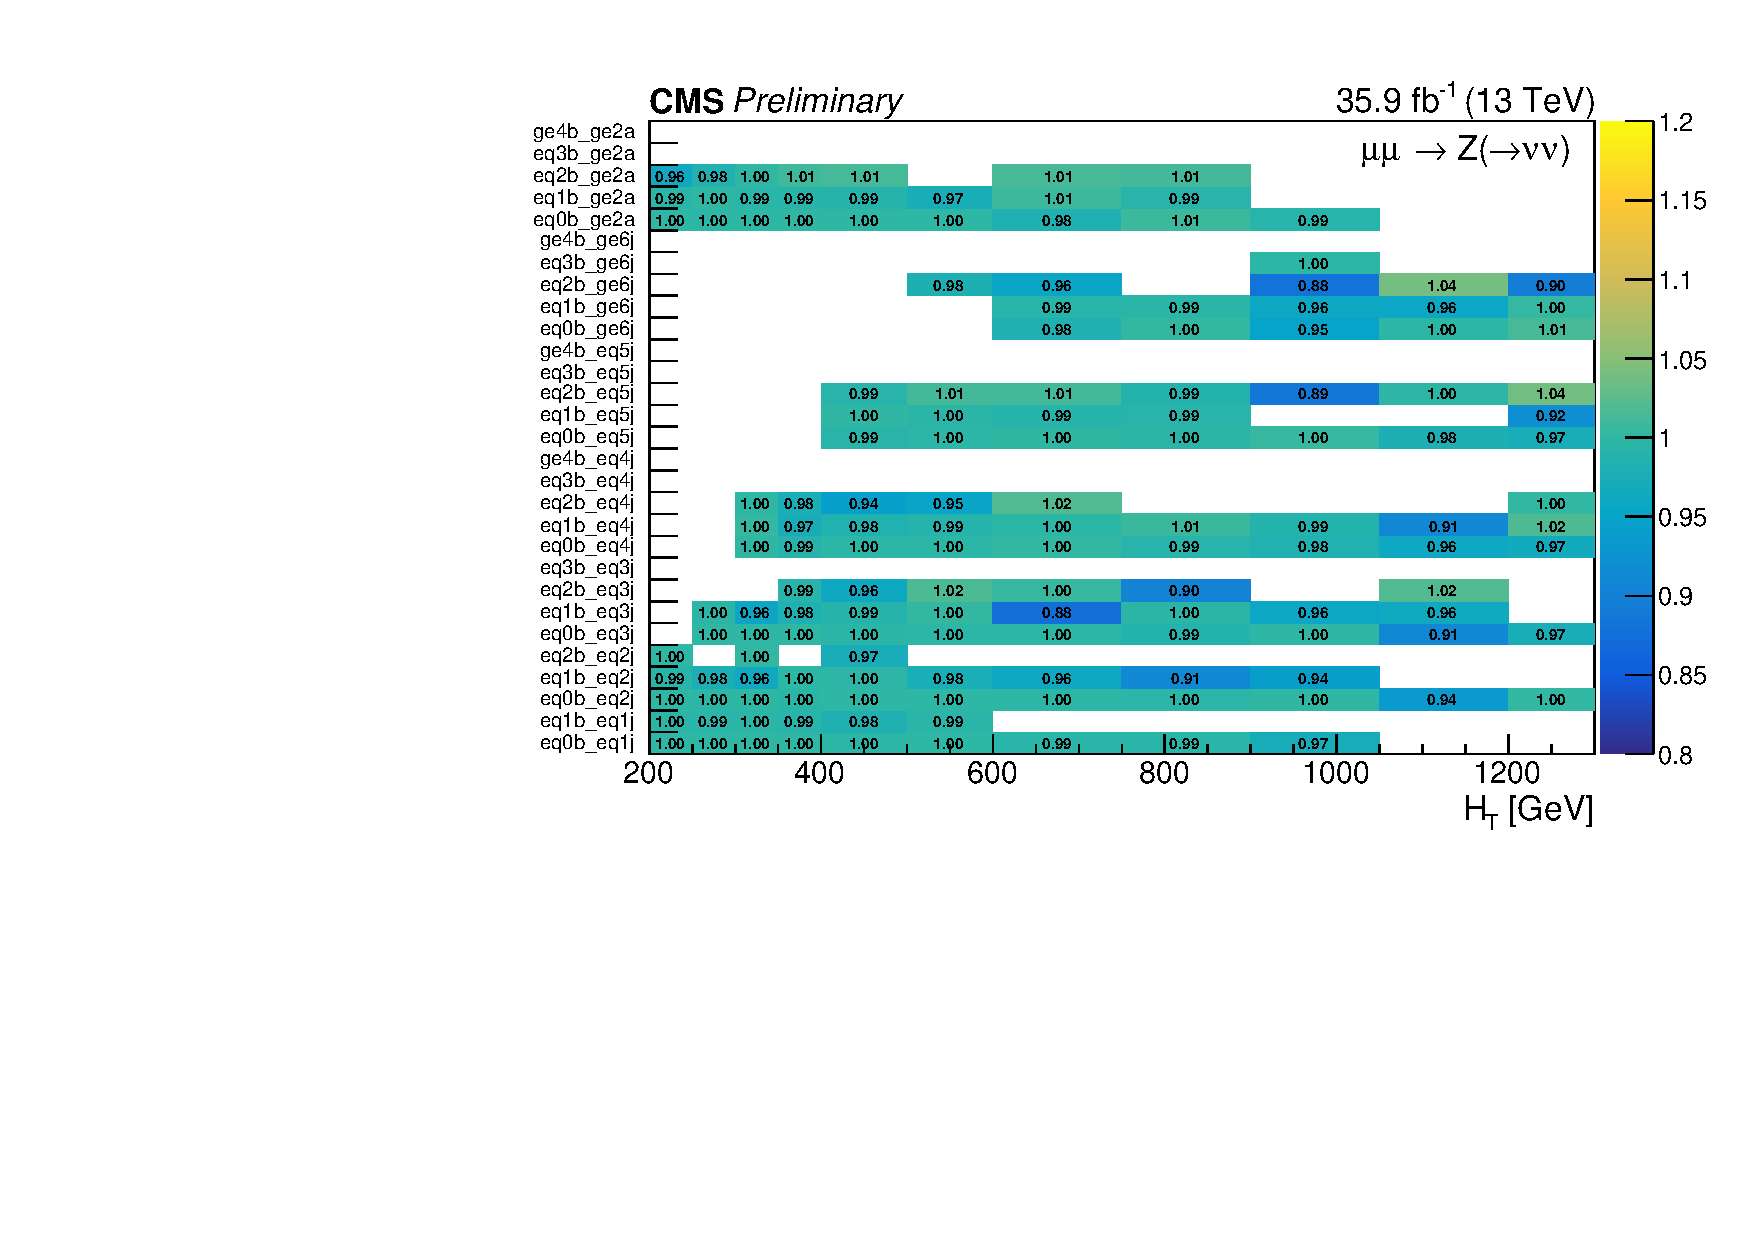
\includegraphics[width=0.5\textwidth]{figures/mcSystematics36p4fb/plots/tfratio_mumu_Zinv_2d_pdfWeightUp.pdf}
  } ~
  \subfigure[Down variation versus (\njet,\nb) category and \scalht.]{
    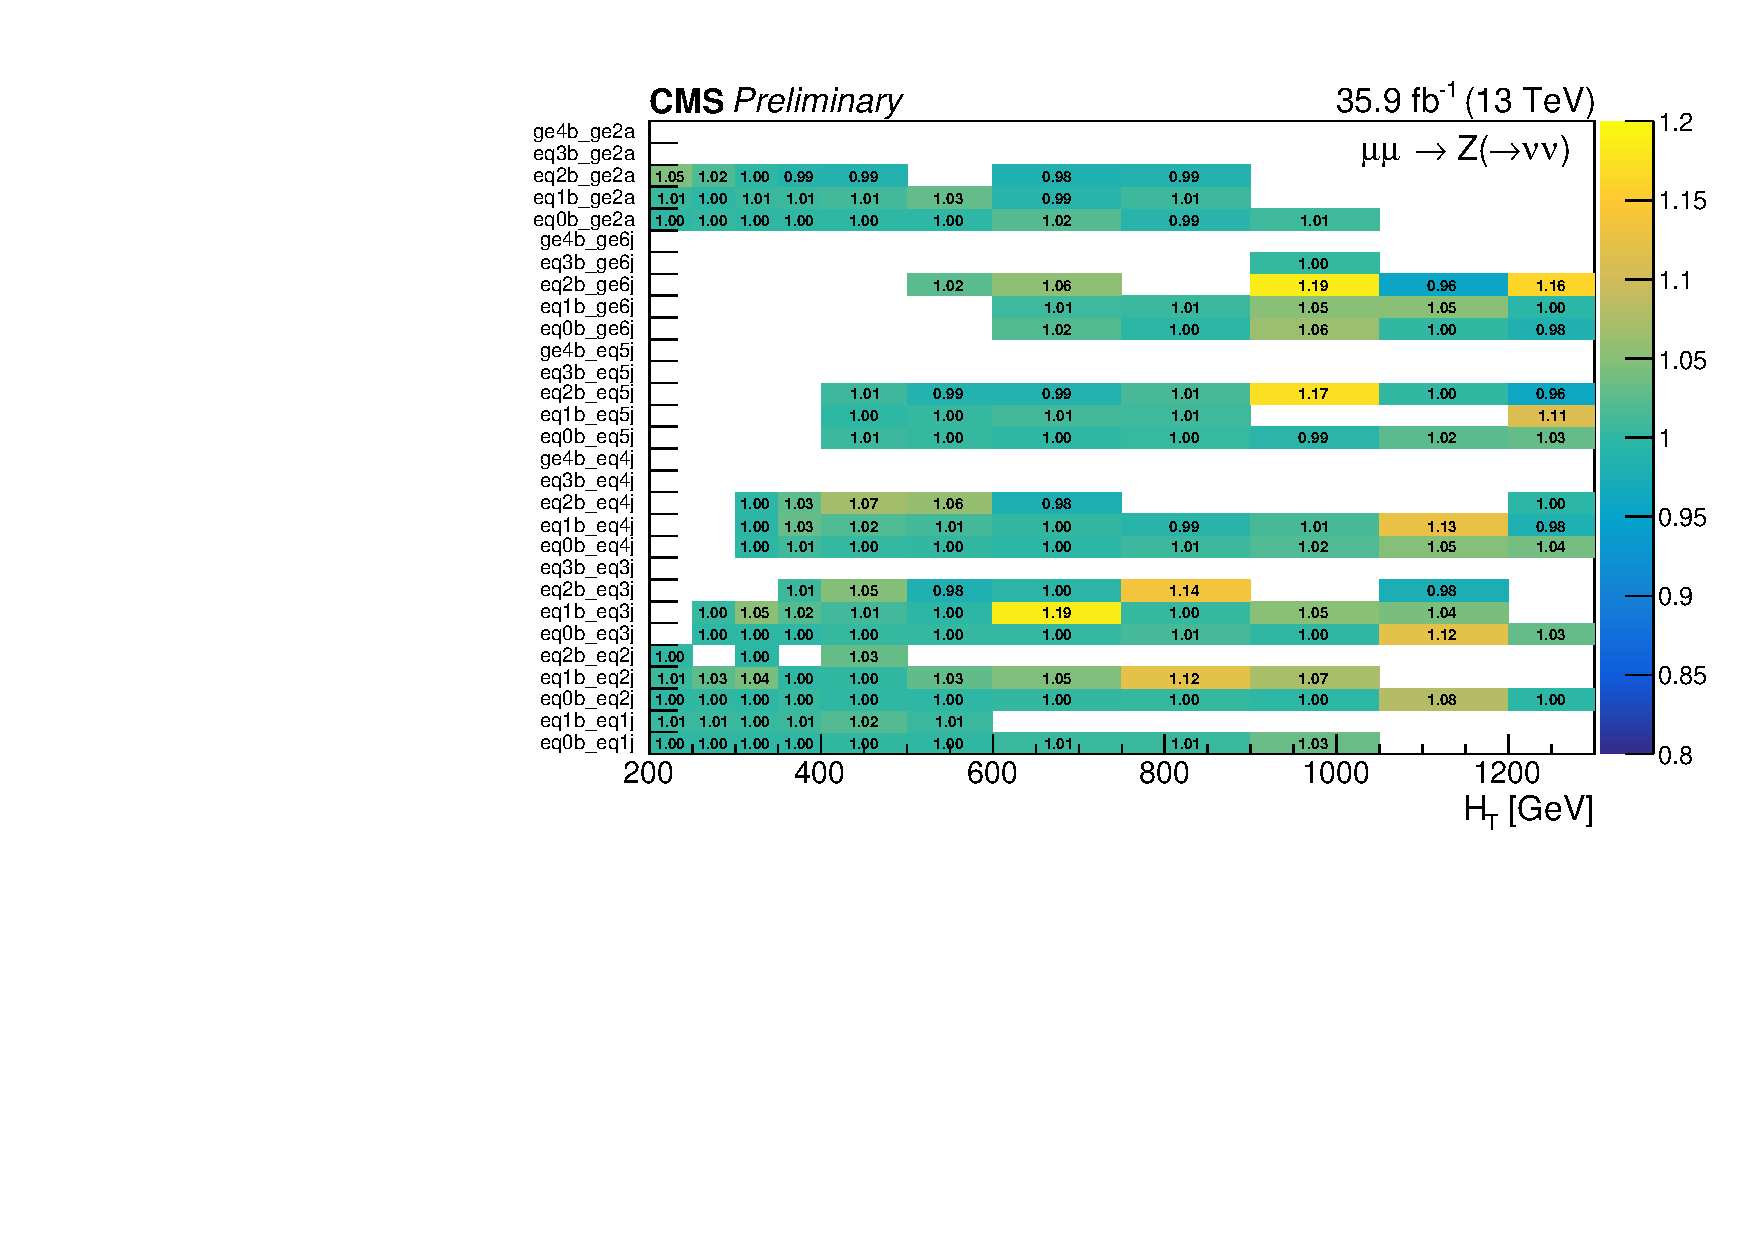
\includegraphics[width=0.5\textwidth]{figures/mcSystematics36p4fb/plots/tfratio_mumu_Zinv_2d_pdfWeightDown.pdf}
  }\\
  \subfigure[Up/down variations versus \njet.]{
    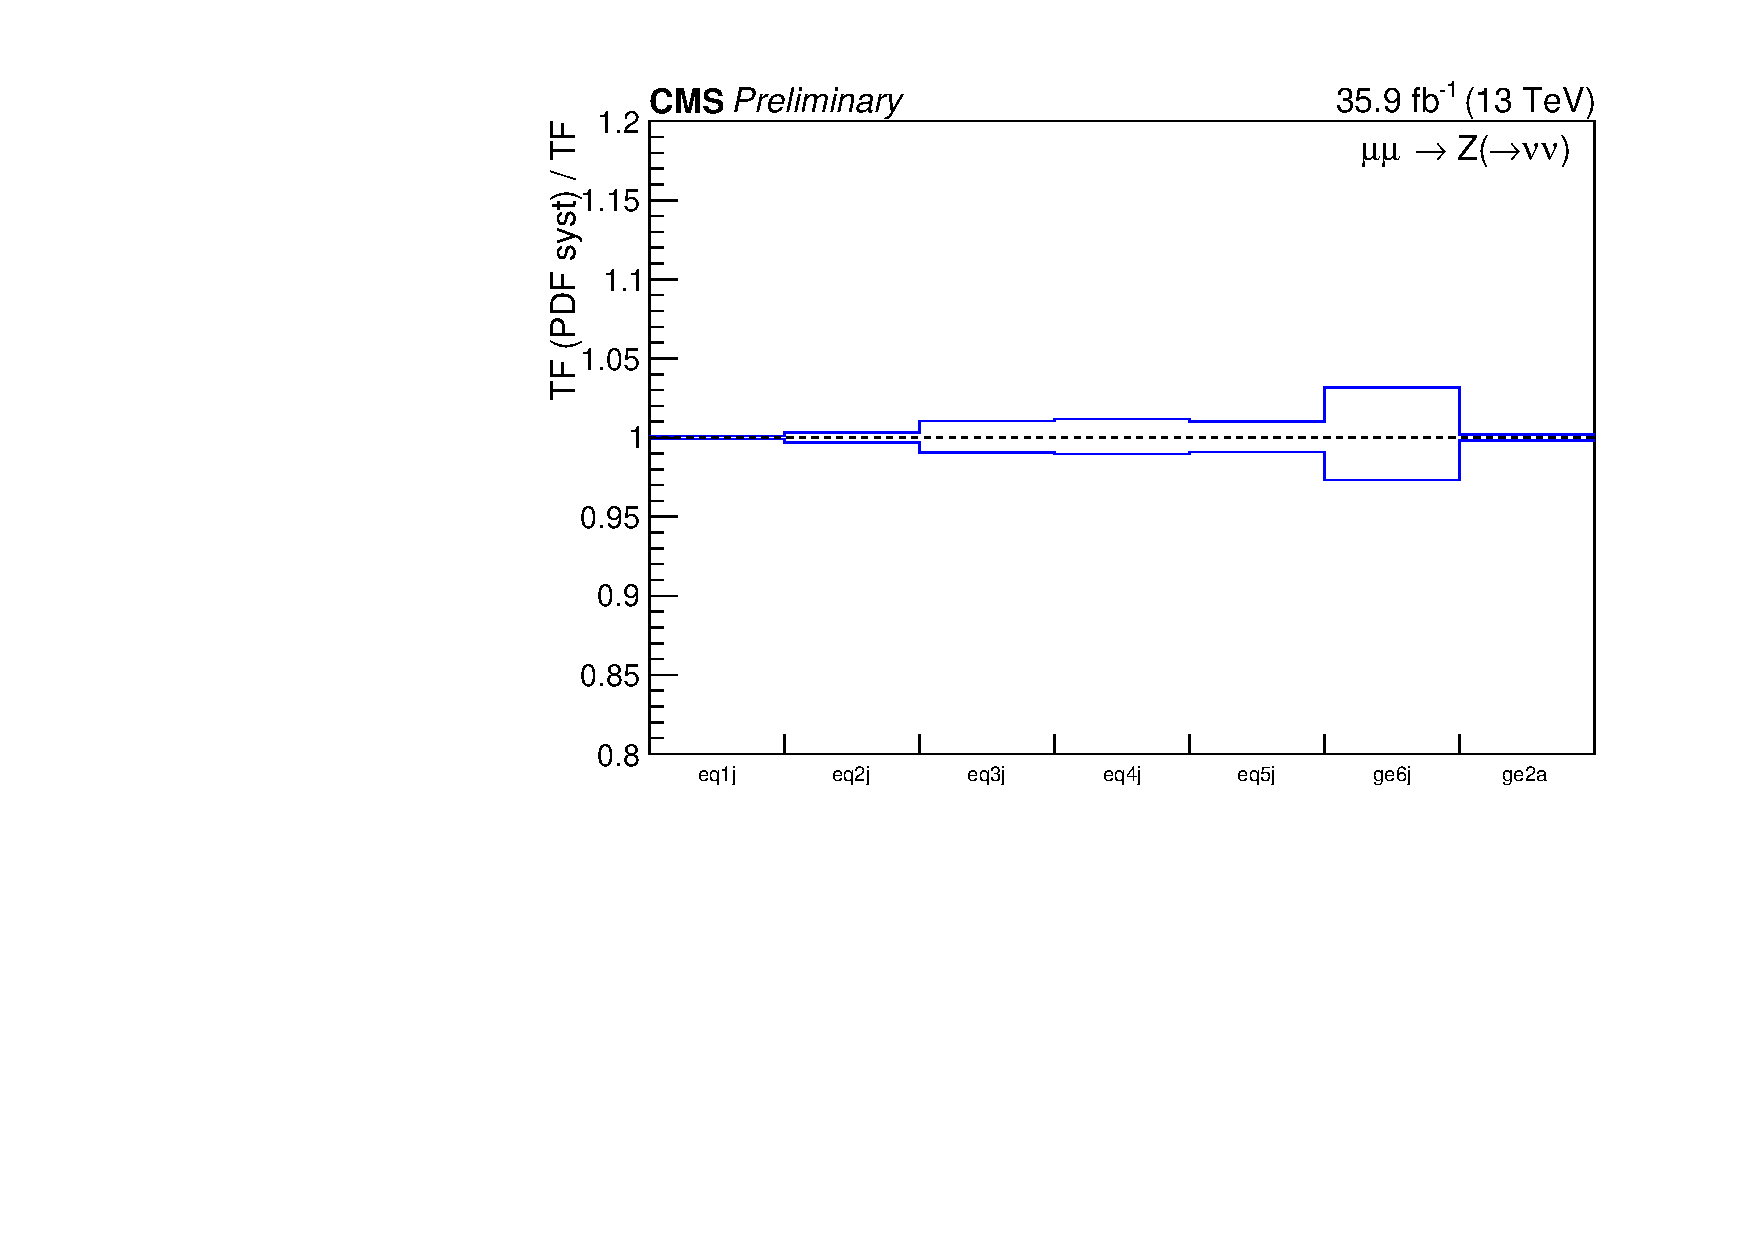
\includegraphics[width=0.5\textwidth]{figures/mcSystematics36p4fb/plots/tfratio_mumu_Zinv_njet_pdfWeightUp.pdf}
  } ~
  \subfigure[Up/down variations versus \scalht.]{
    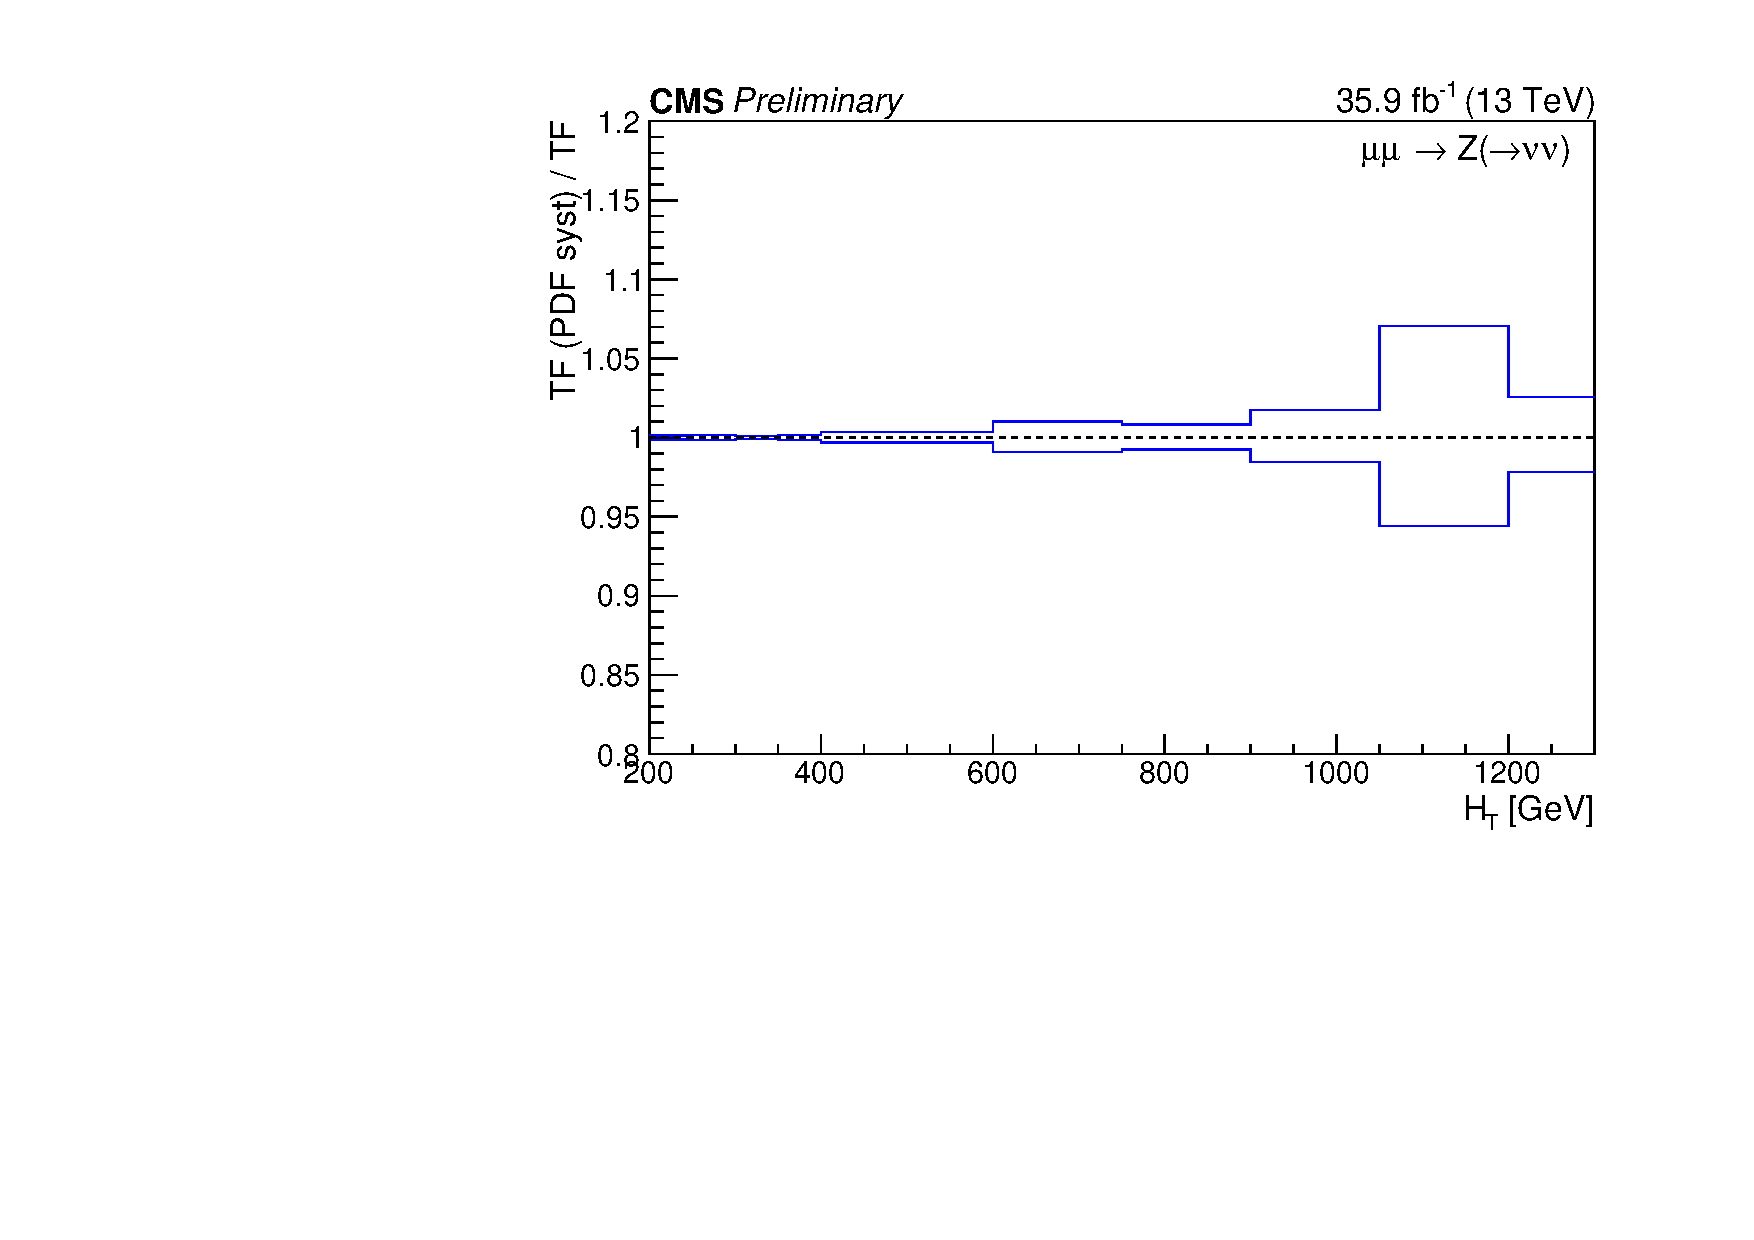
\includegraphics[width=0.5\textwidth]{figures/mcSystematics36p4fb/plots/tfratio_mumu_Zinv_ht_pdfWeightUp.pdf}
  } \\
  \subfigure[Up/down variations versus \nb.]{
    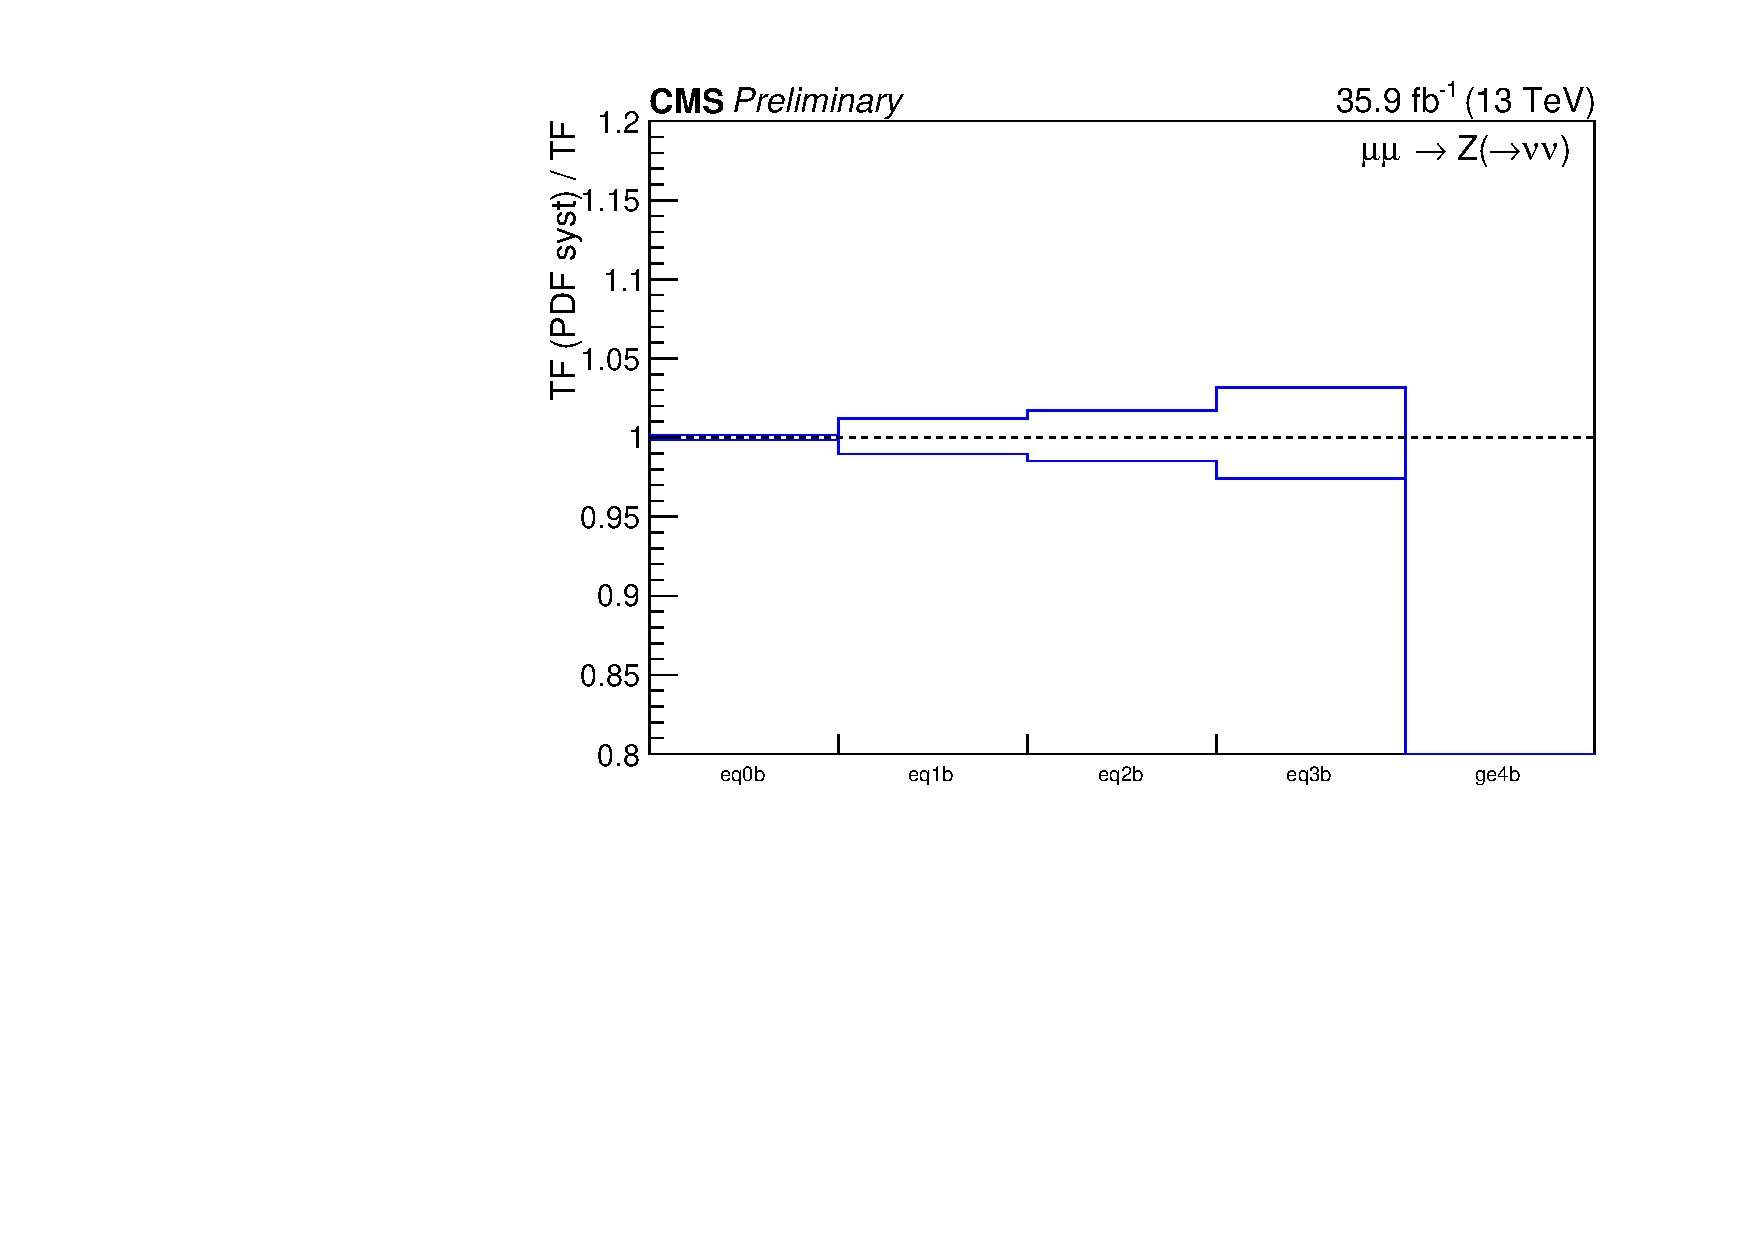
\includegraphics[width=0.5\textwidth]{figures/mcSystematics36p4fb/plots/tfratio_mumu_Zinv_bjet_pdfWeightUp.pdf}
  } ~
  \subfigure[Up/down variations versus \mht.]{
    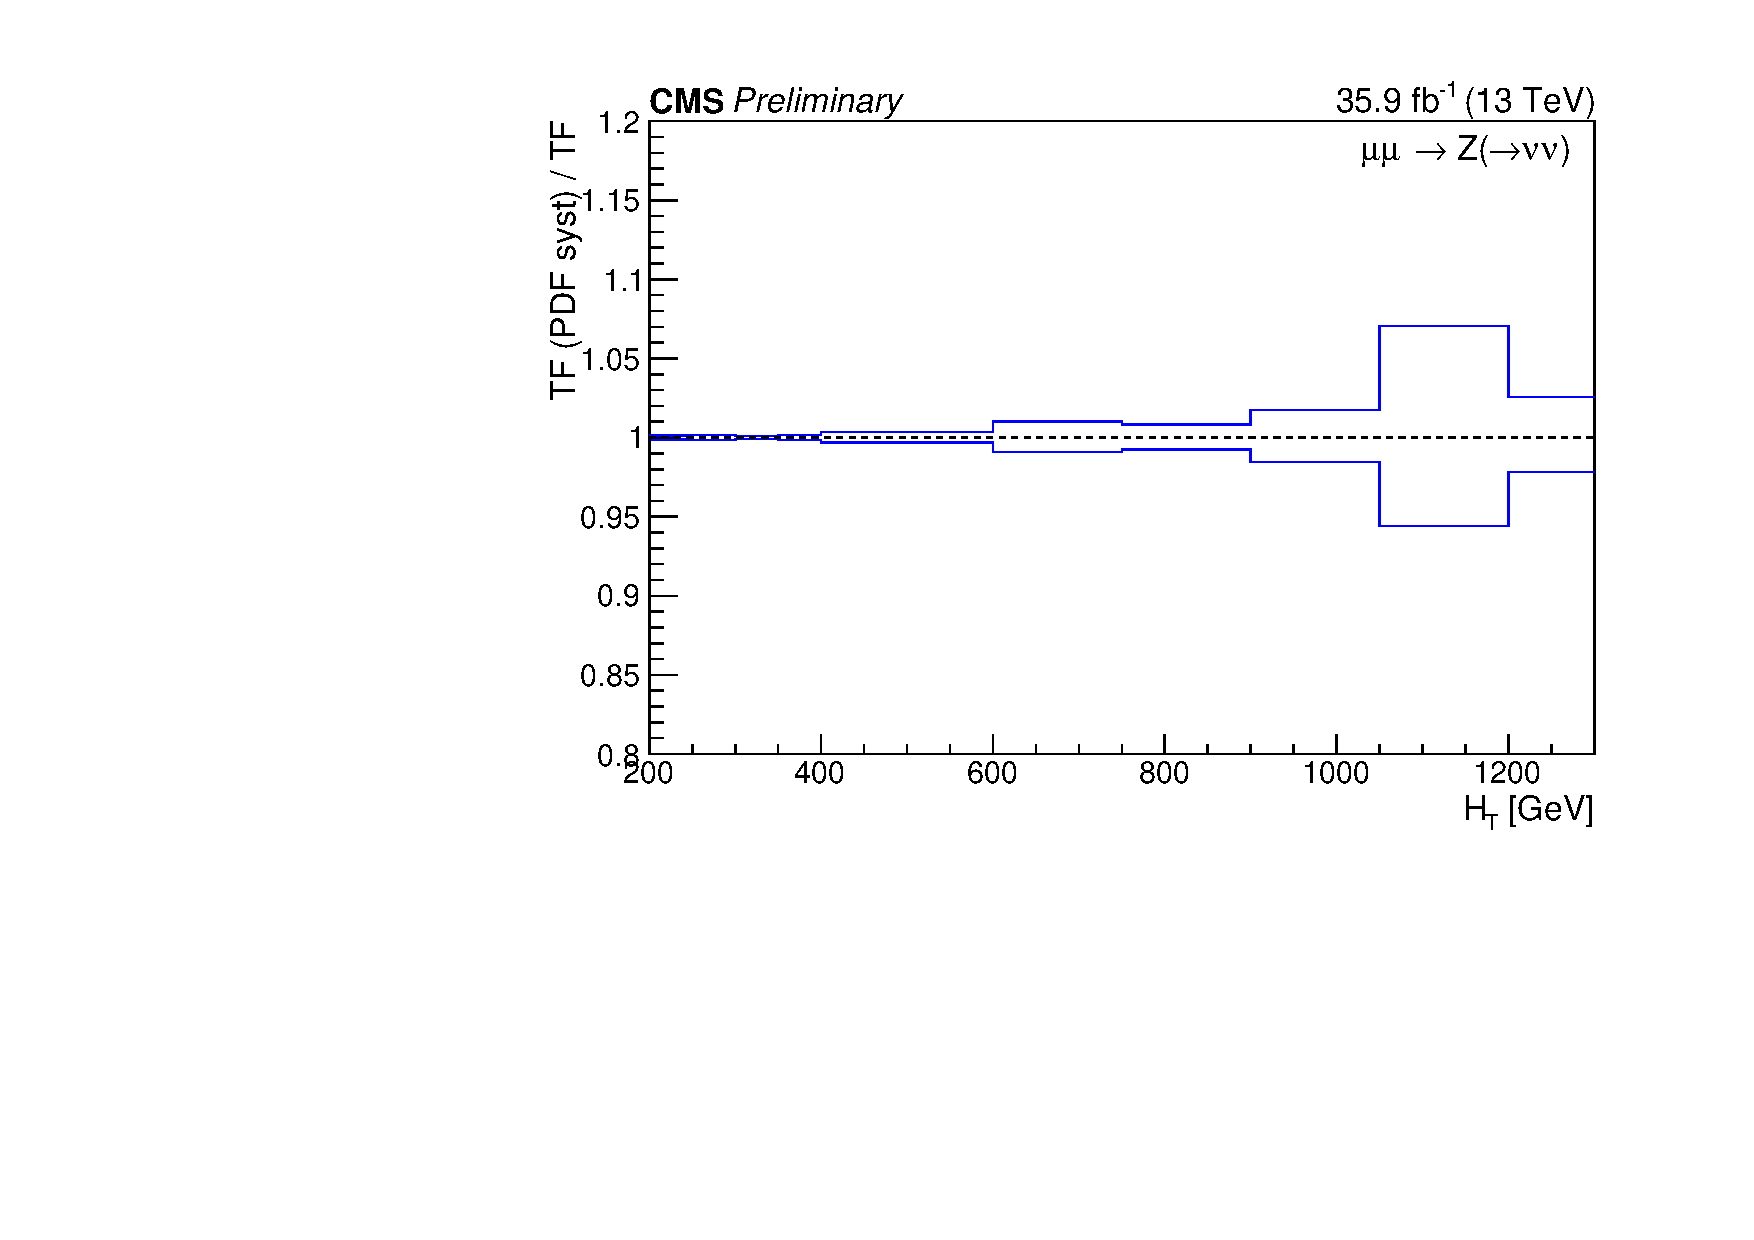
\includegraphics[width=0.5\textwidth]{figures/mcSystematics36p4fb/plots/tfratio_mumu_Zinv_ht_pdfWeightUp.pdf}
  } \\
  \caption{\label{fig:tfSyst_pdf_mumuToZinv} The relative change in the
    ``$\mmj \rightarrow \znunu\ + \textrm{jets}$'' transfer factors from
    simulation due to $\pm1\sigma$ uncertainties in parton density
    functions.  } 
\end{figure}

\clearpage
\subsection{Missing higher-order corrections in LO \texorpdfstring{\MADGRAPH}{MadGraph}
  samples}

\begin{figure}[!h]
  \centering
  \subfigure[Correction versus Z boson \Pt.]{
    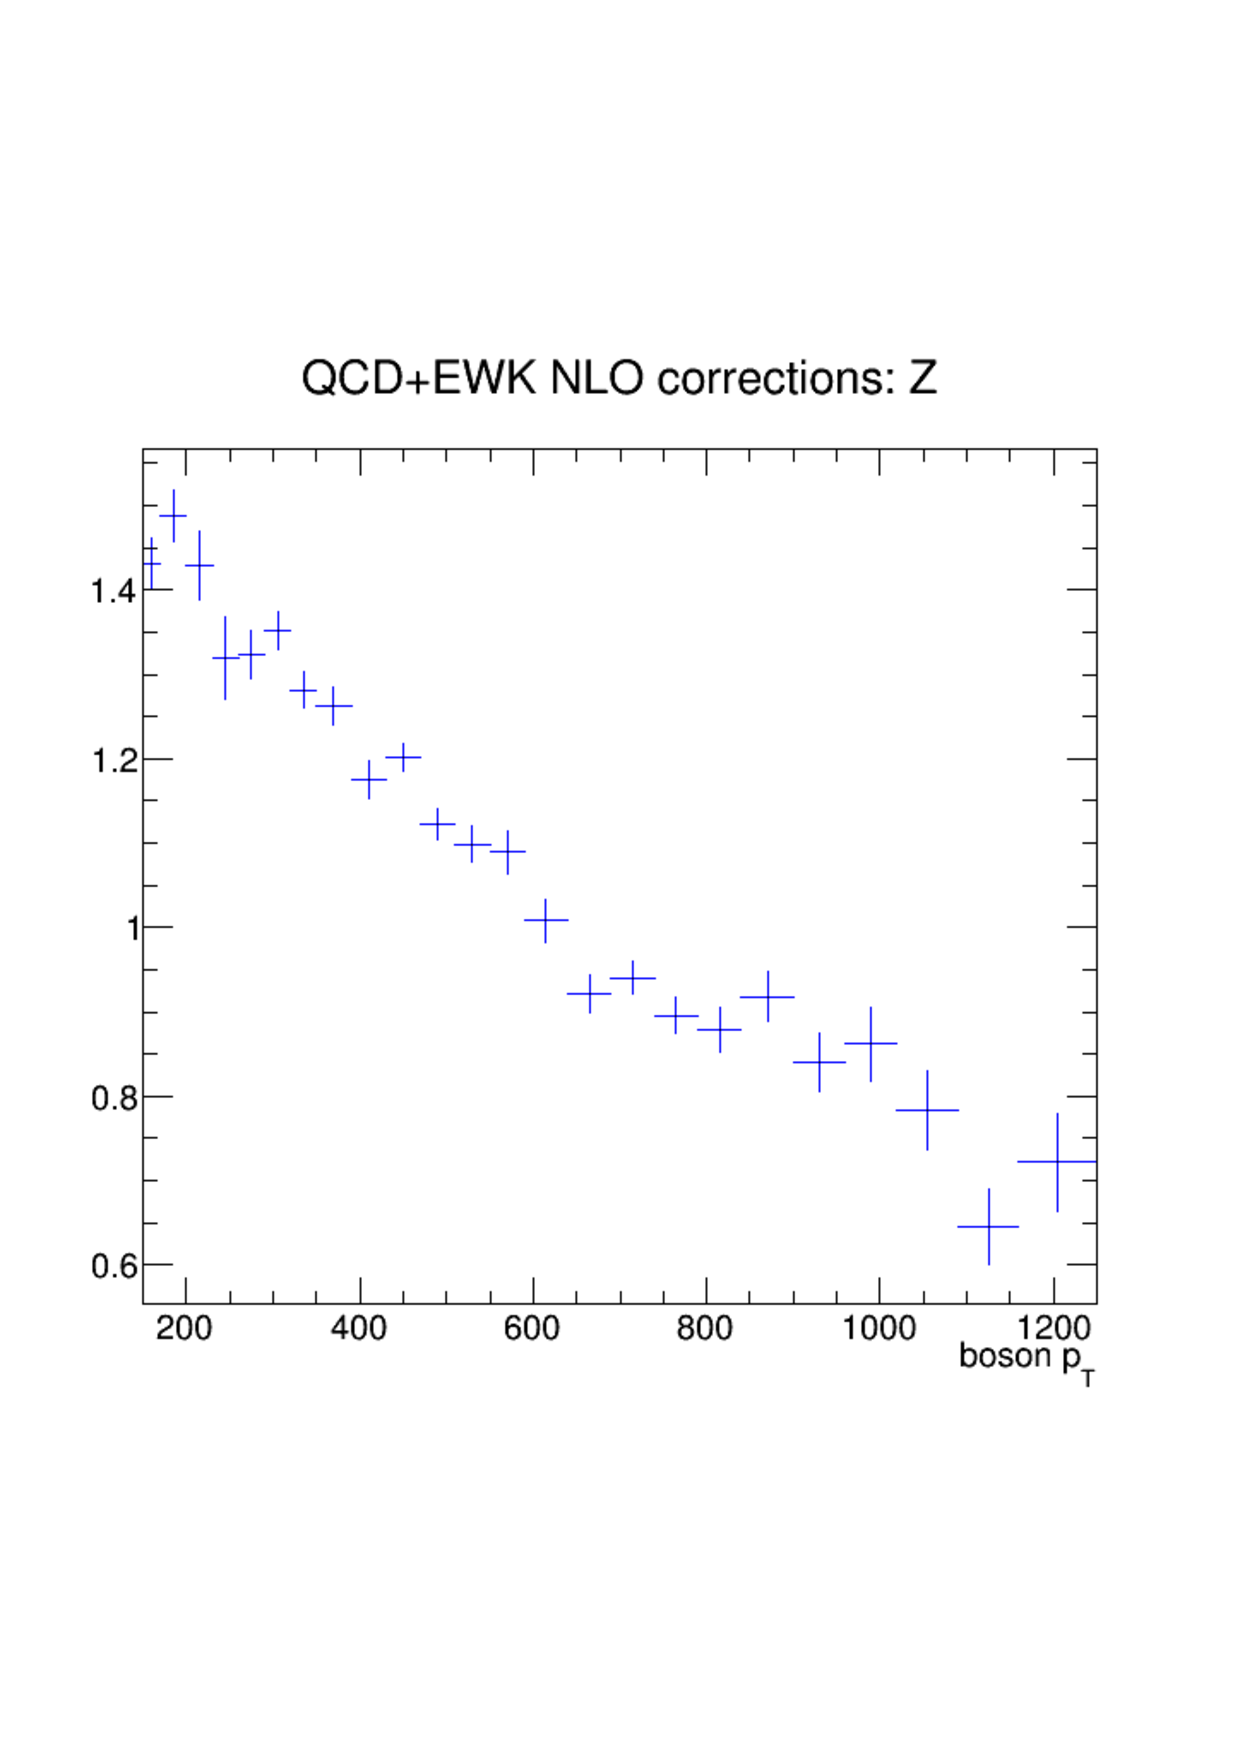
\includegraphics[width=0.4\textwidth,trim=0 150 0 150,crop]{figures/NLO/Z.pdf}
  } ~
  \subfigure[Variation versus (\njet,\nb) category and \scalht.]{
    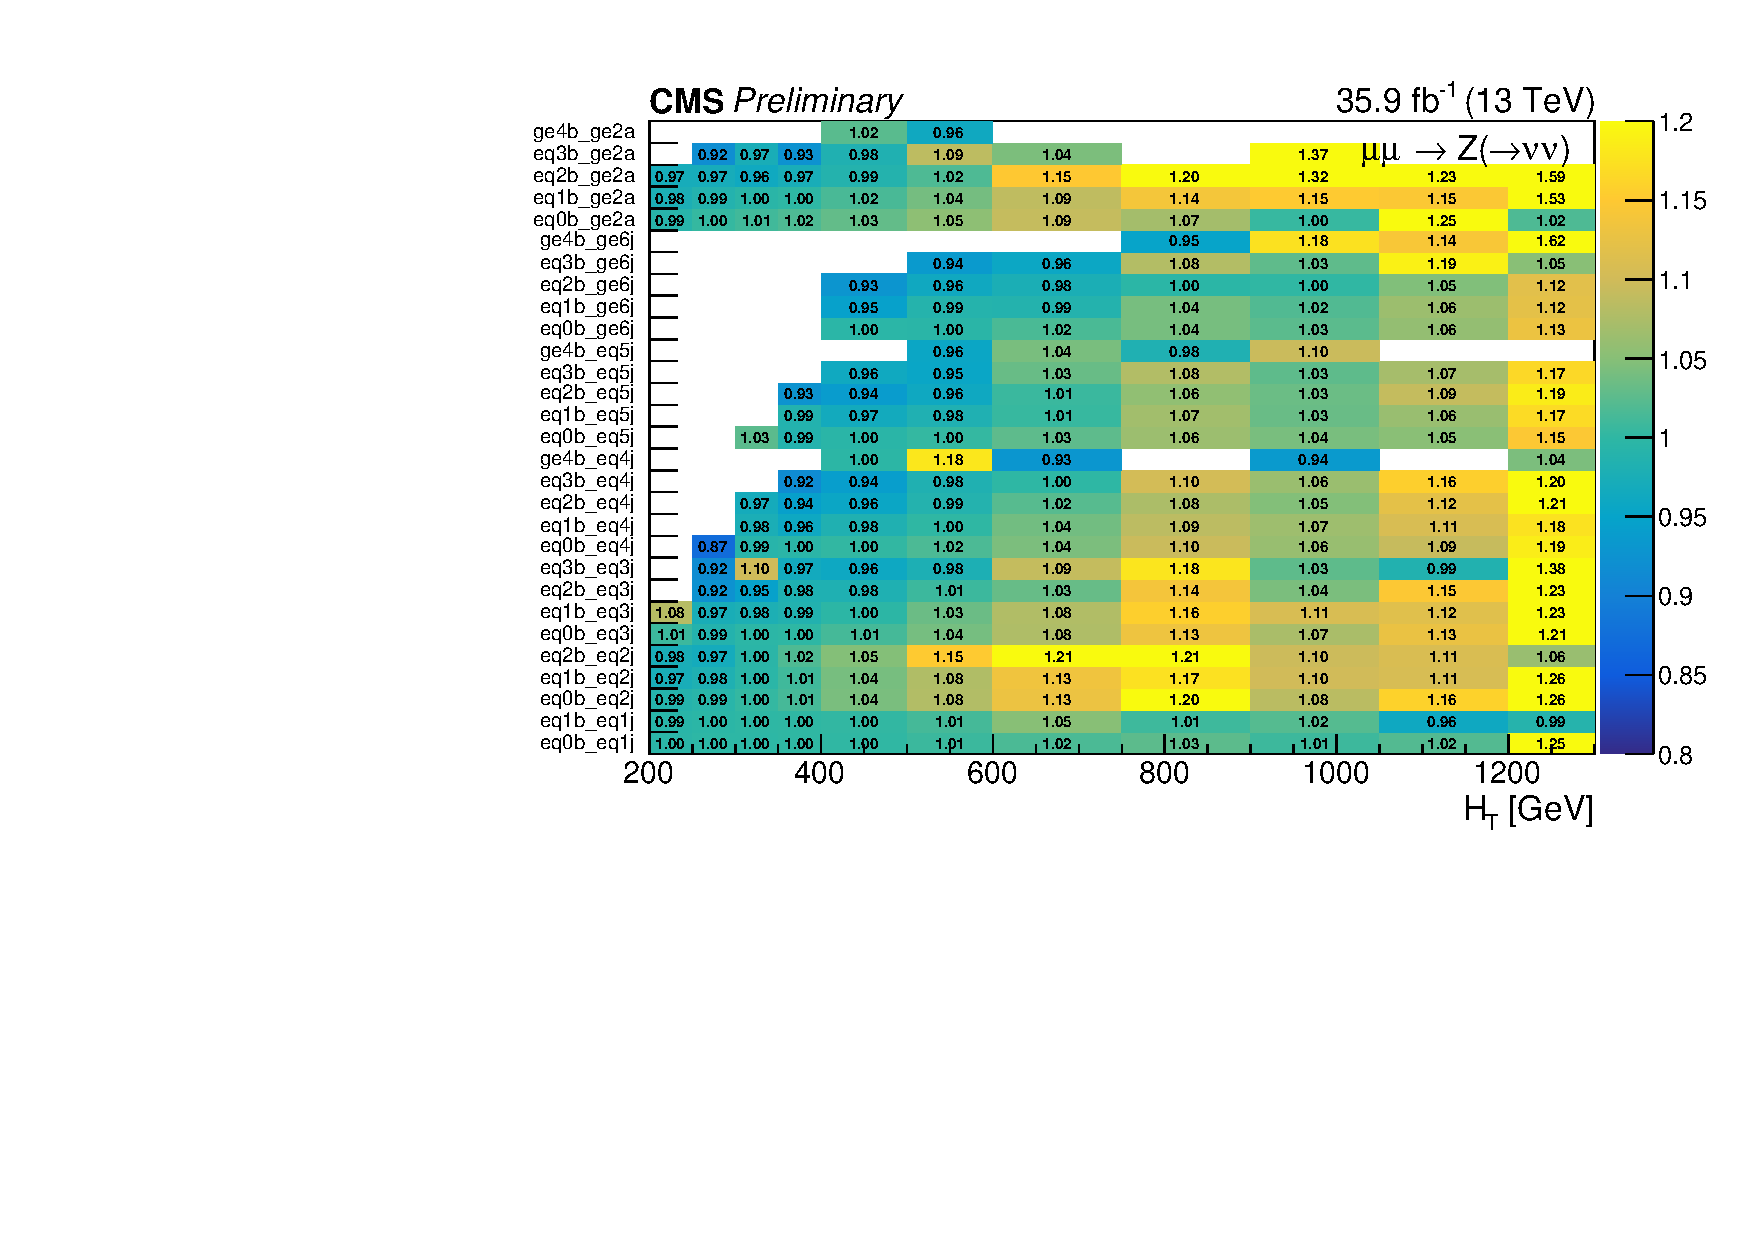
\includegraphics[width=0.5\textwidth]{figures/mcSystematics36p4fb/plots/tfratio_mumu_Zinv_2d_bosonPtWeightDown.pdf}
  }\\
  \subfigure[Variation versus \njet.]{
    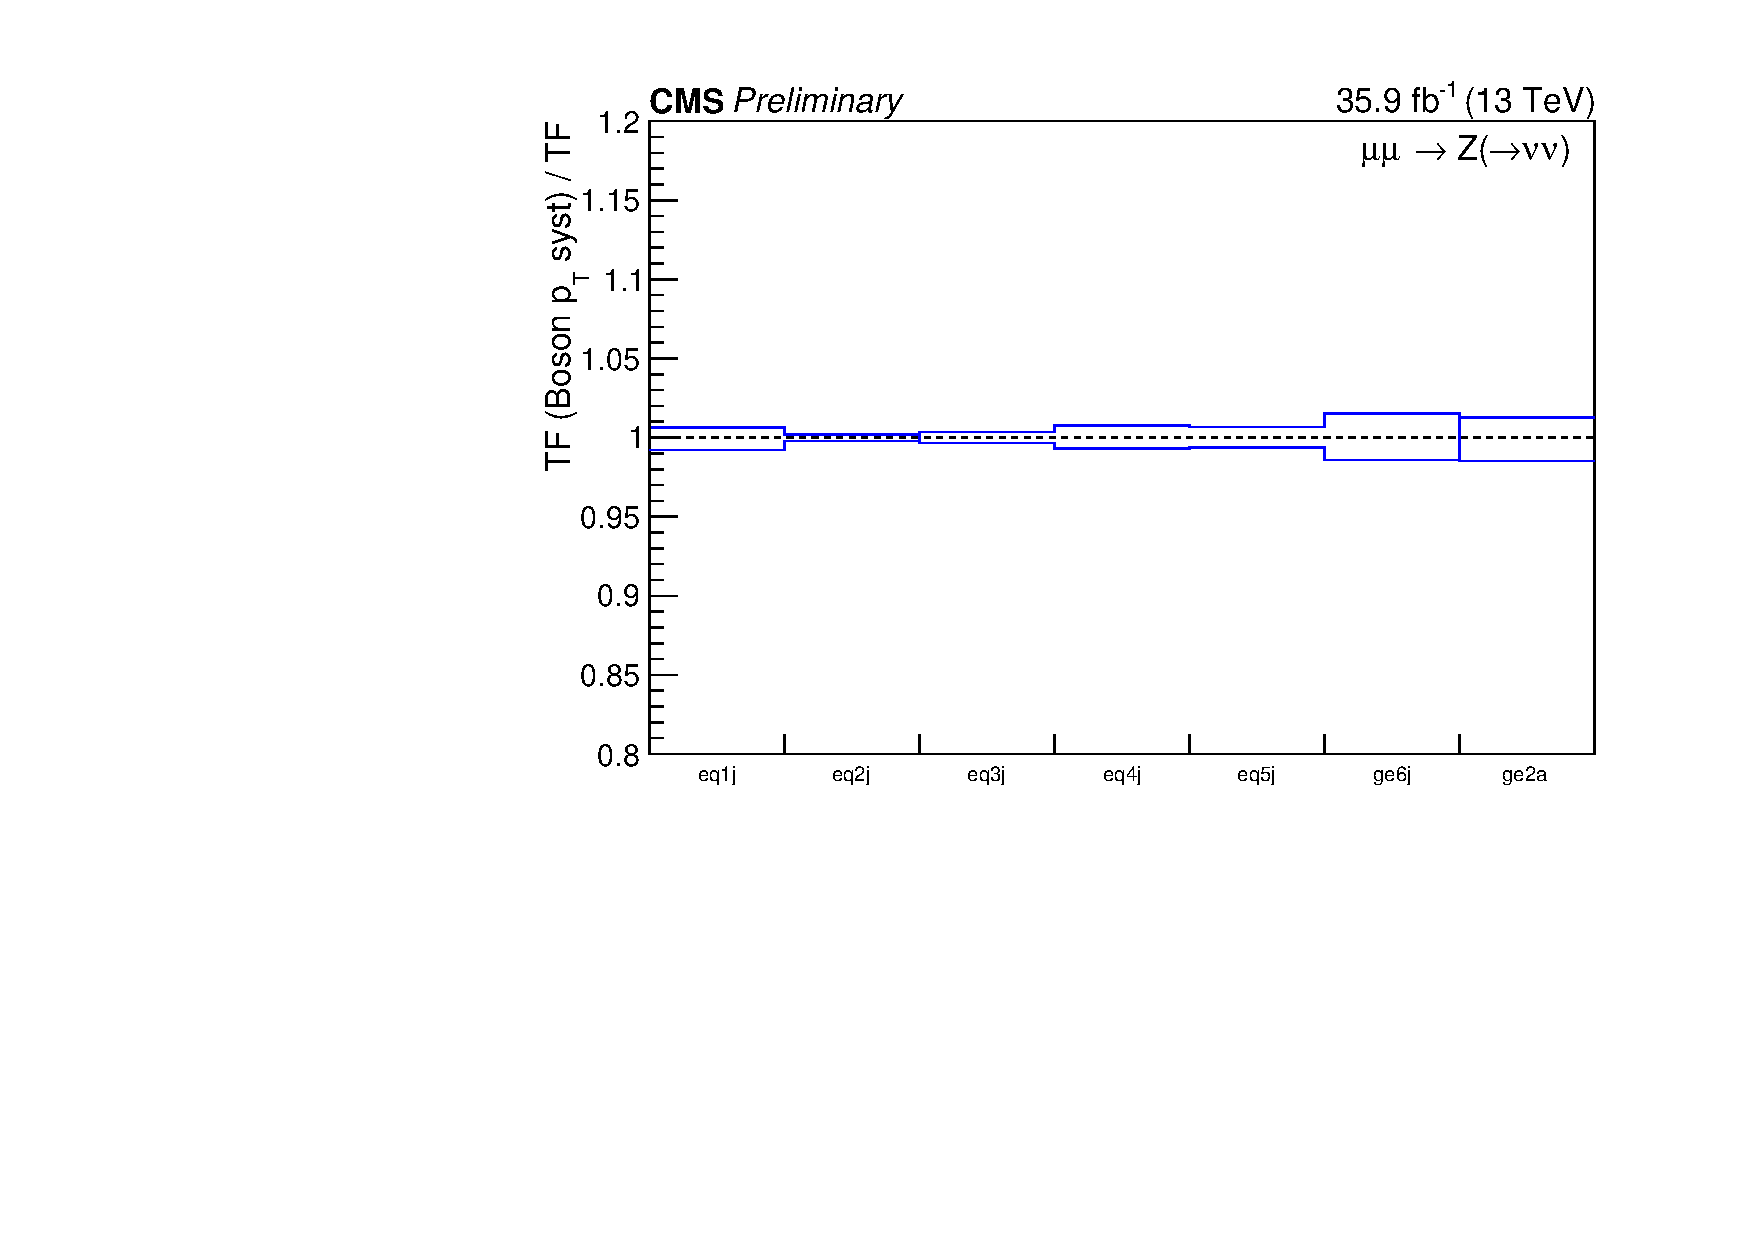
\includegraphics[width=0.5\textwidth]{figures/mcSystematics36p4fb/plots/tfratio_mumu_Zinv_njet_bosonPtWeightUp.pdf}
  } ~
  \subfigure[Variation versus \scalht.]{
    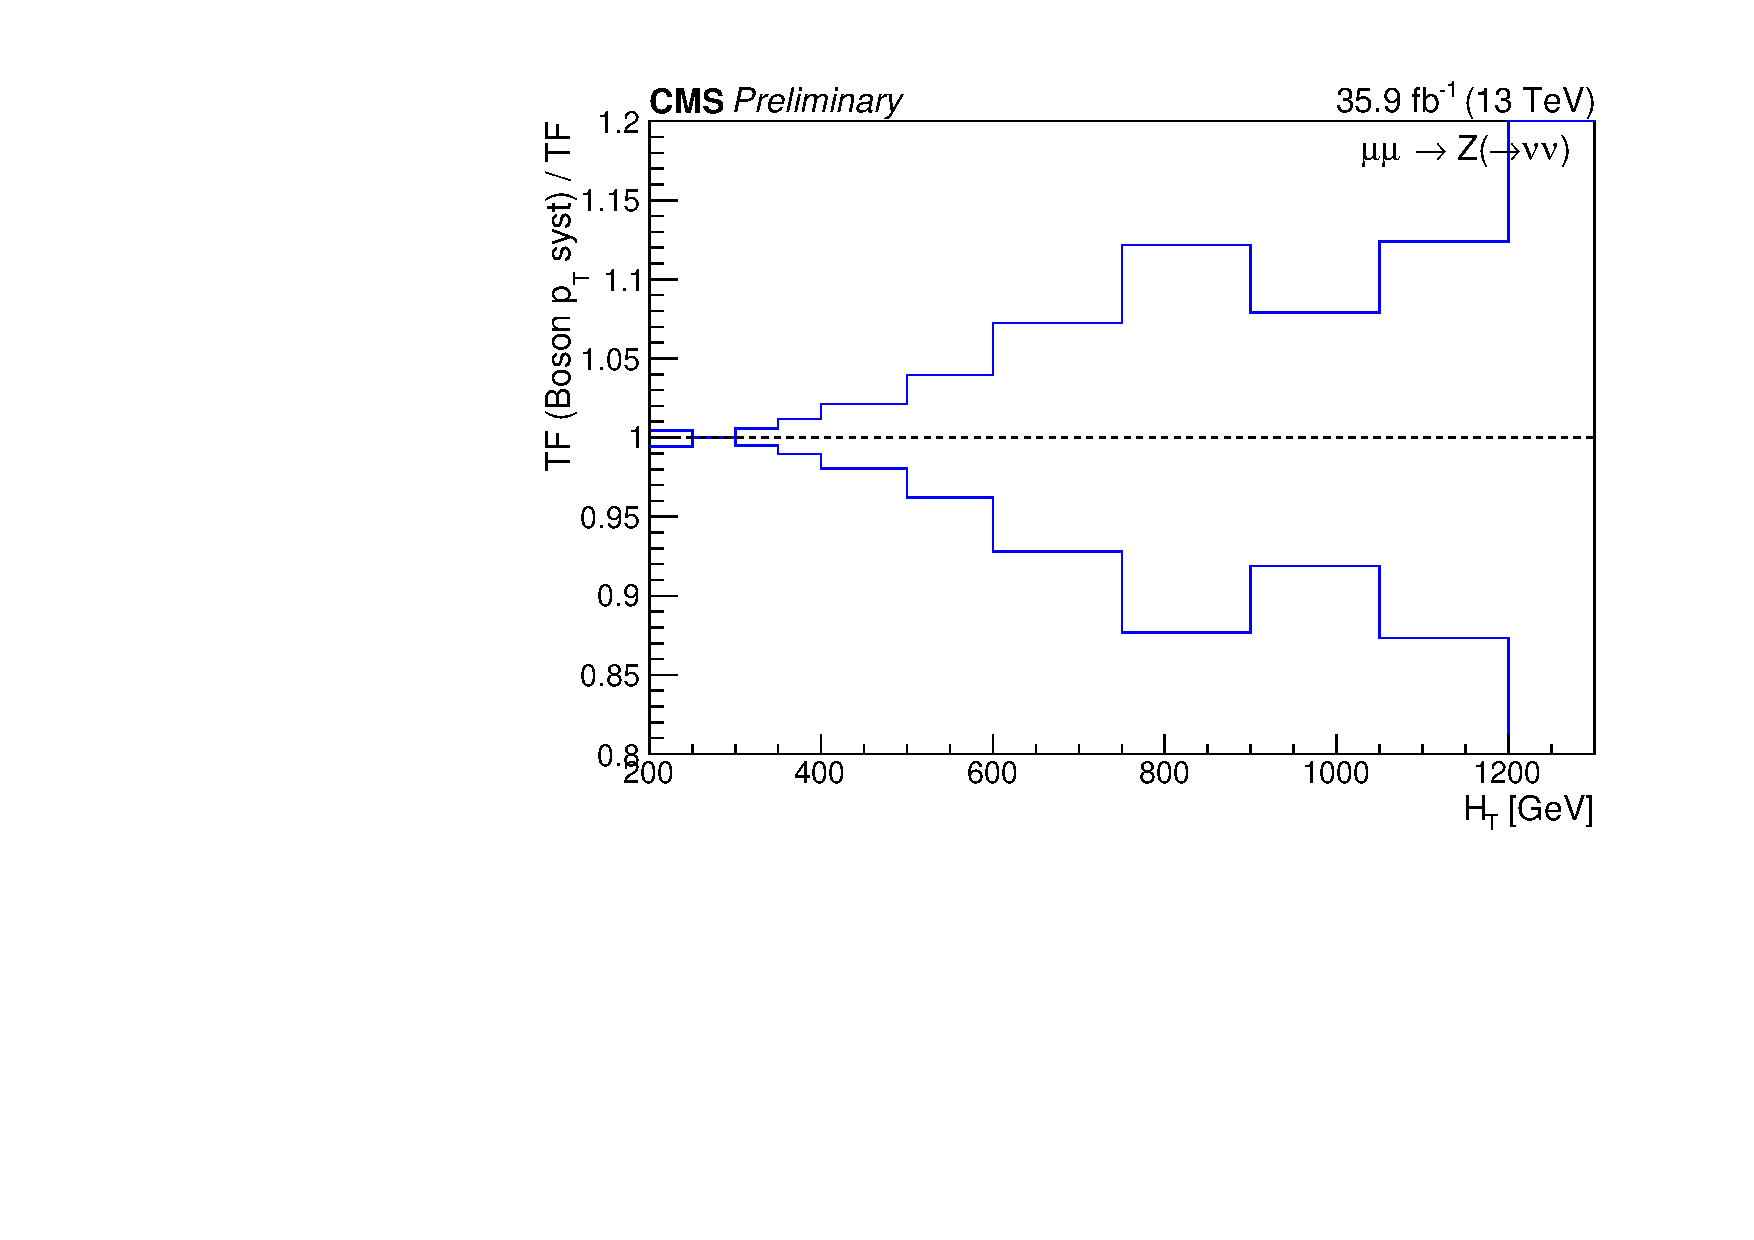
\includegraphics[width=0.5\textwidth]{figures/mcSystematics36p4fb/plots/tfratio_mumu_Zinv_ht_bosonPtWeightUp.pdf}
  } \\
  \subfigure[Variation versus \nb.]{
    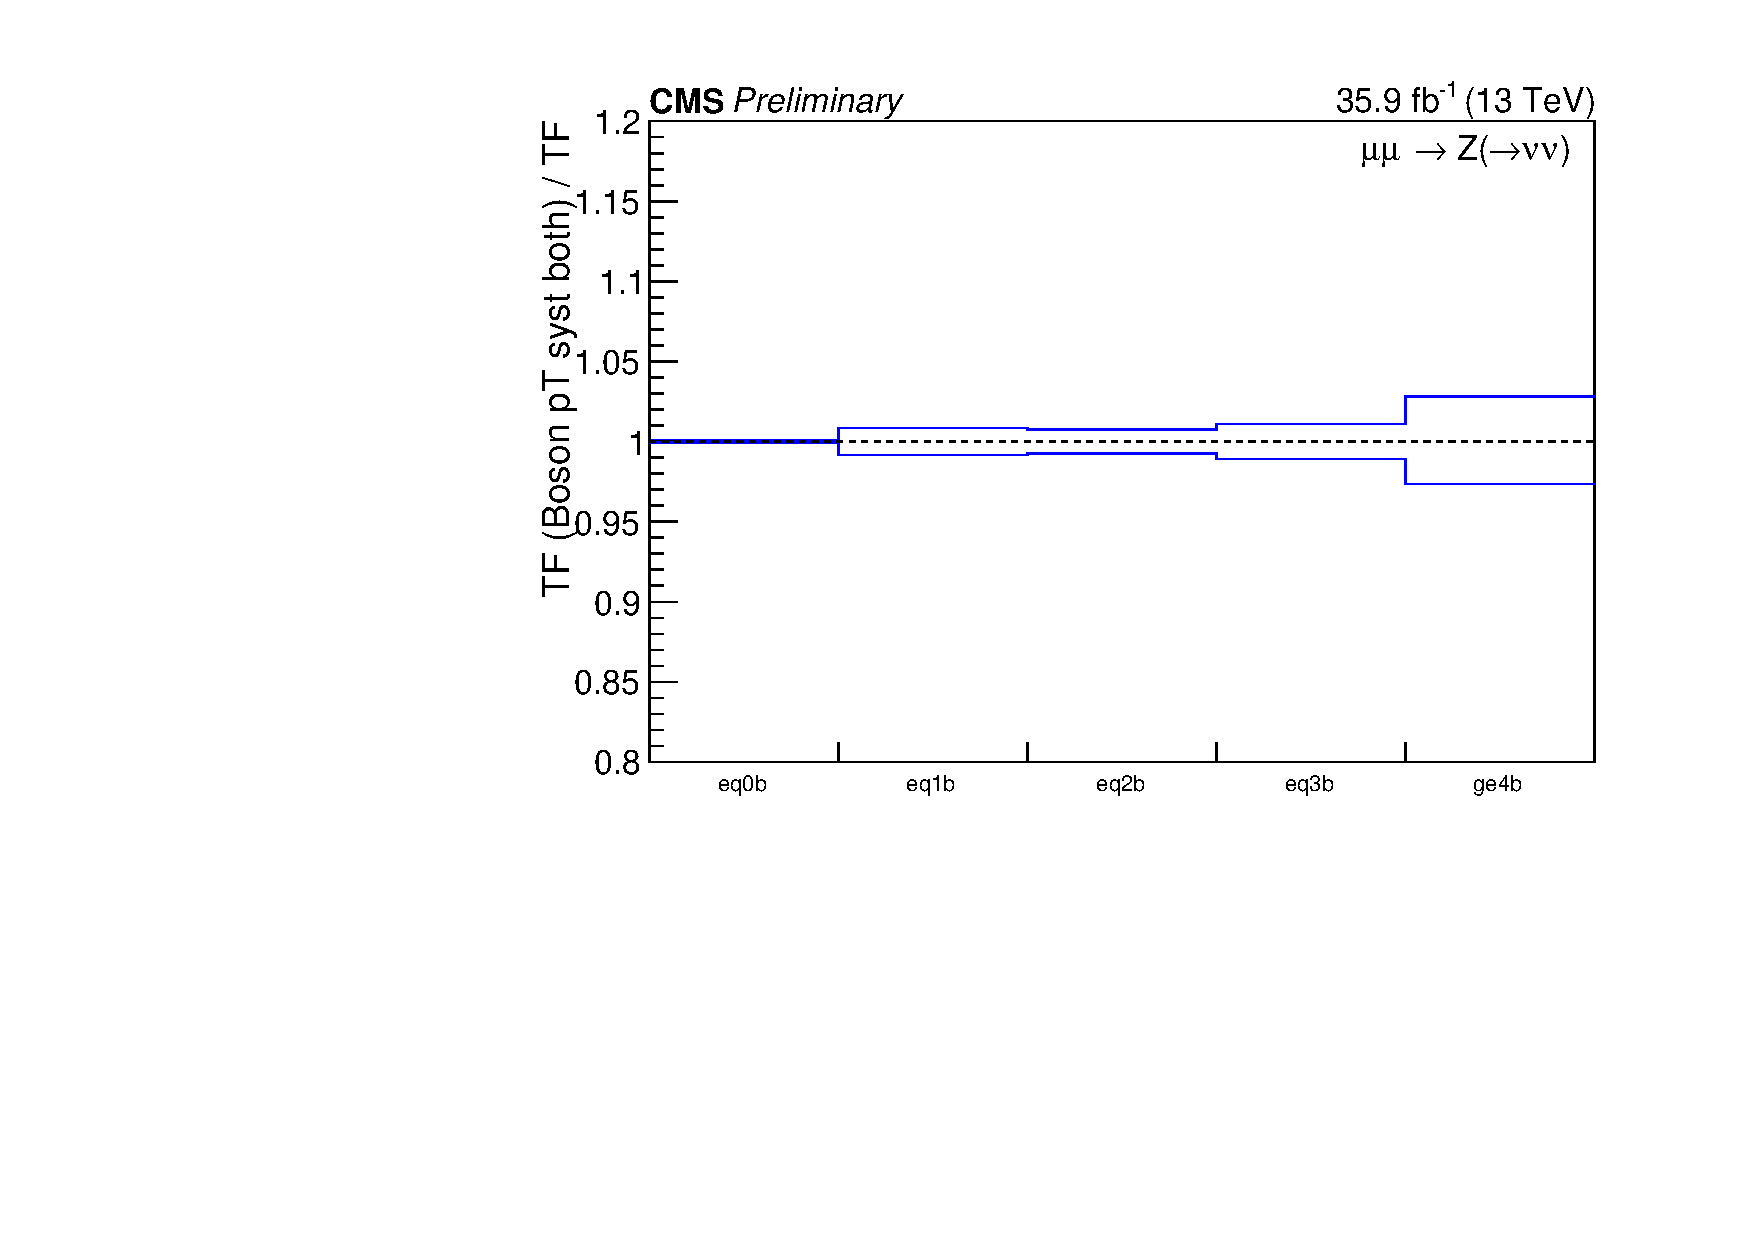
\includegraphics[width=0.5\textwidth]{figures/mcSystematics36p4fb/plots/tfratio_mumu_Zinv_bjet_bosonPtWeightUp.pdf}
  } ~
  \subfigure[Variation versus \mht.]{
    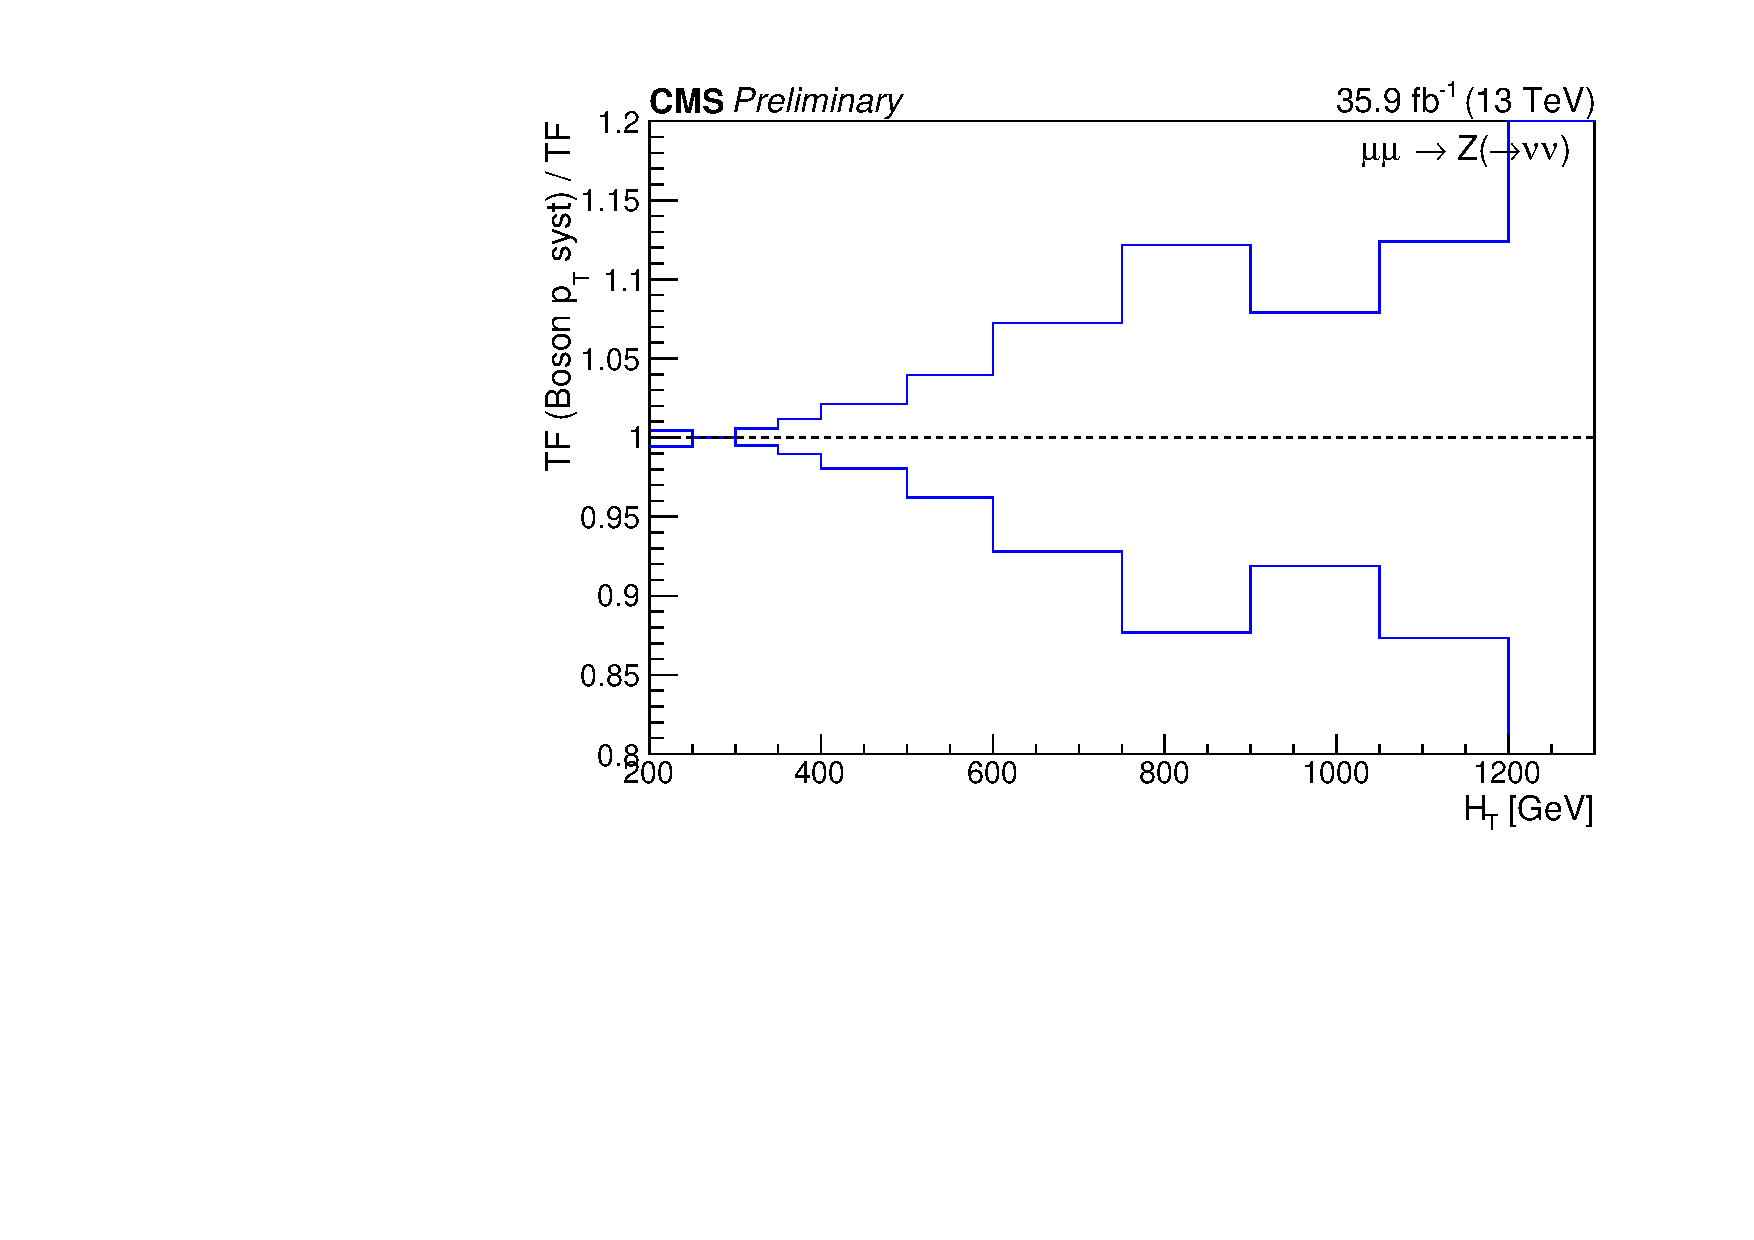
\includegraphics[width=0.5\textwidth]{figures/mcSystematics36p4fb/plots/tfratio_mumu_Zinv_ht_bosonPtWeightUp.pdf}
  } \\
  \caption{\label{fig:tfSyst_nlo_mumuToZinv} The relative change in the
    ``$\mmj \rightarrow \znunu\ + \textrm{jets}$'' transfer factors from
    simulation when assuming uncertainties equal in magnitude to QCD +
    EWK NLO corrections versus Z boson \Pt.  }
\end{figure}

\clearpage
\subsection{Signal trigger efficiency}

\begin{figure}[!h]
  \centering
  \subfigure[Up variation versus (\njet,\nb) category and \scalht.]{
    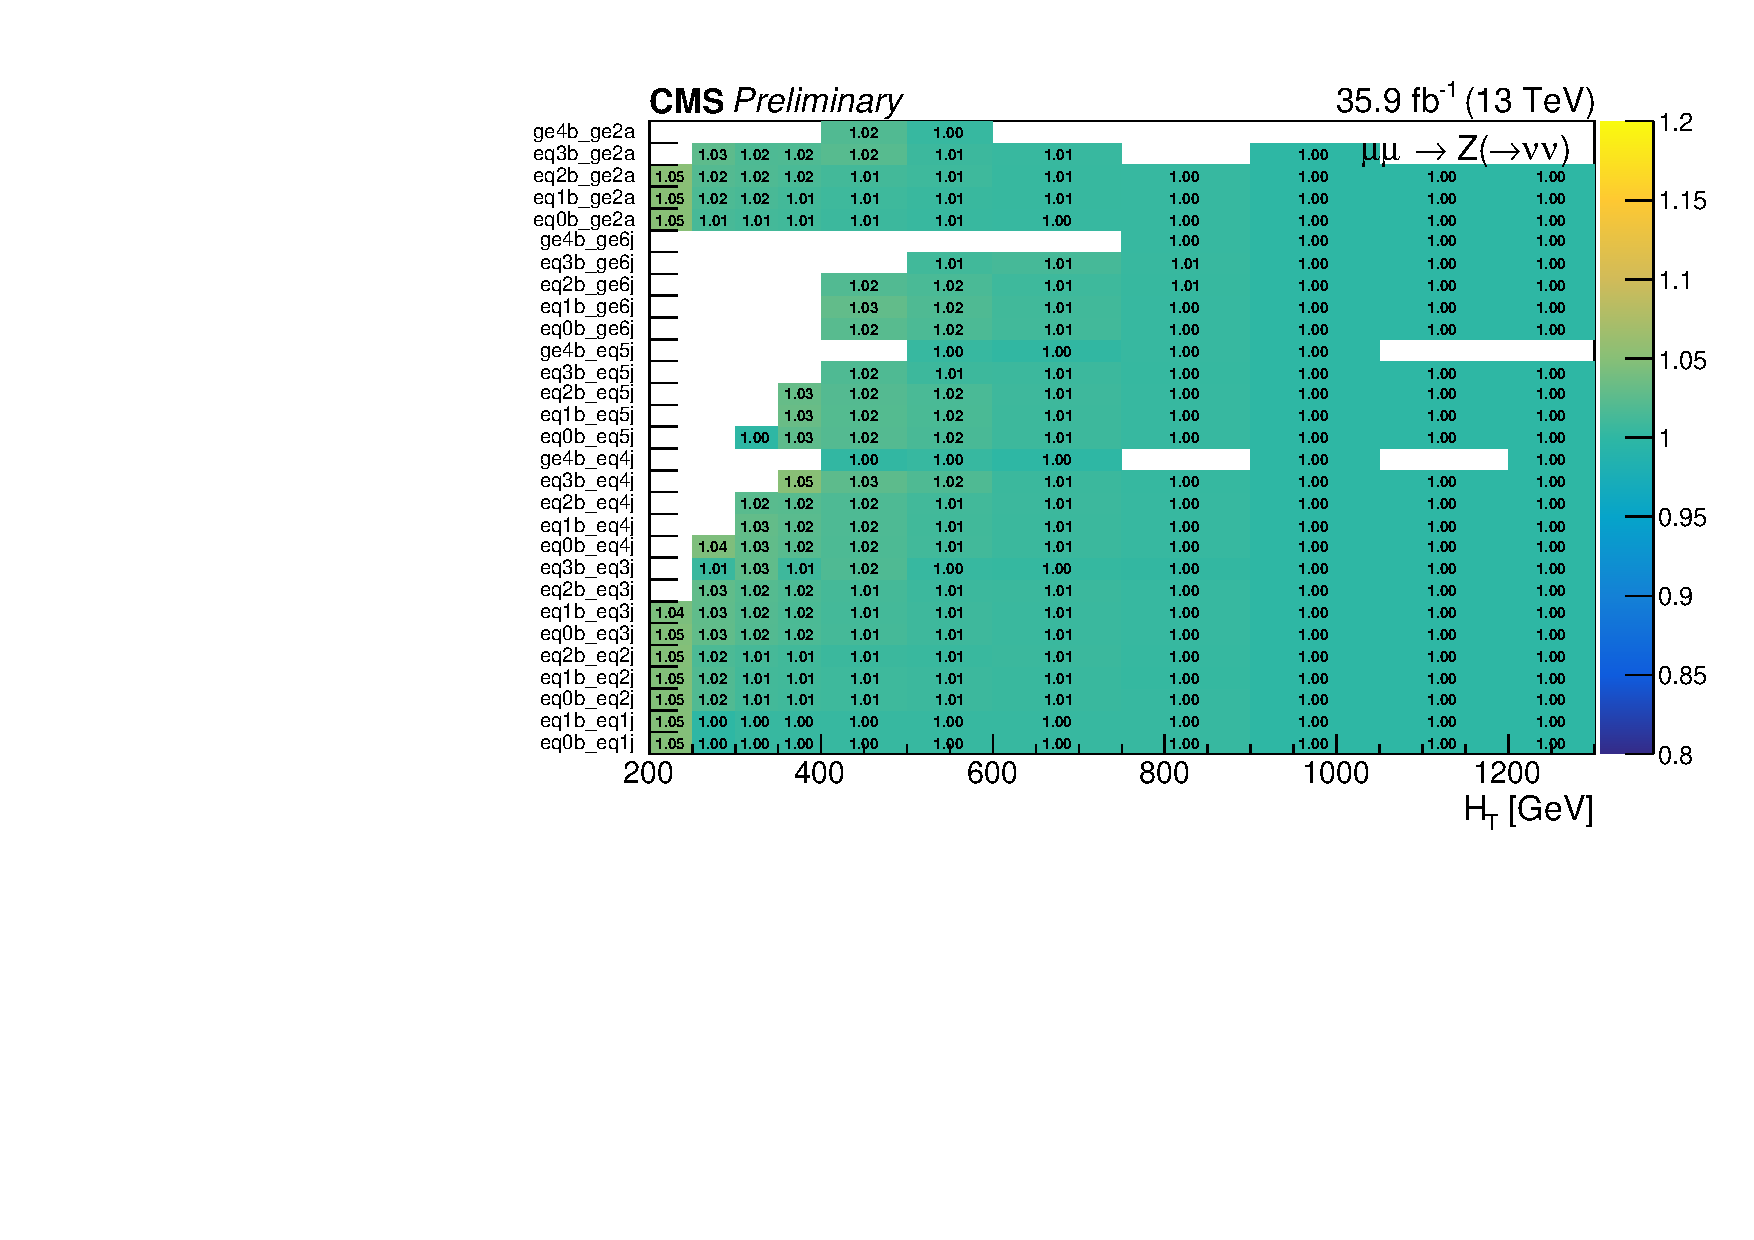
\includegraphics[width=0.5\textwidth]{figures/mcSystematics36p4fb/plots/tfratio_mumu_Zinv_2d_triggerWeightUp.pdf}
  } ~
  \subfigure[Down variation versus (\njet,\nb) category and \scalht.]{
    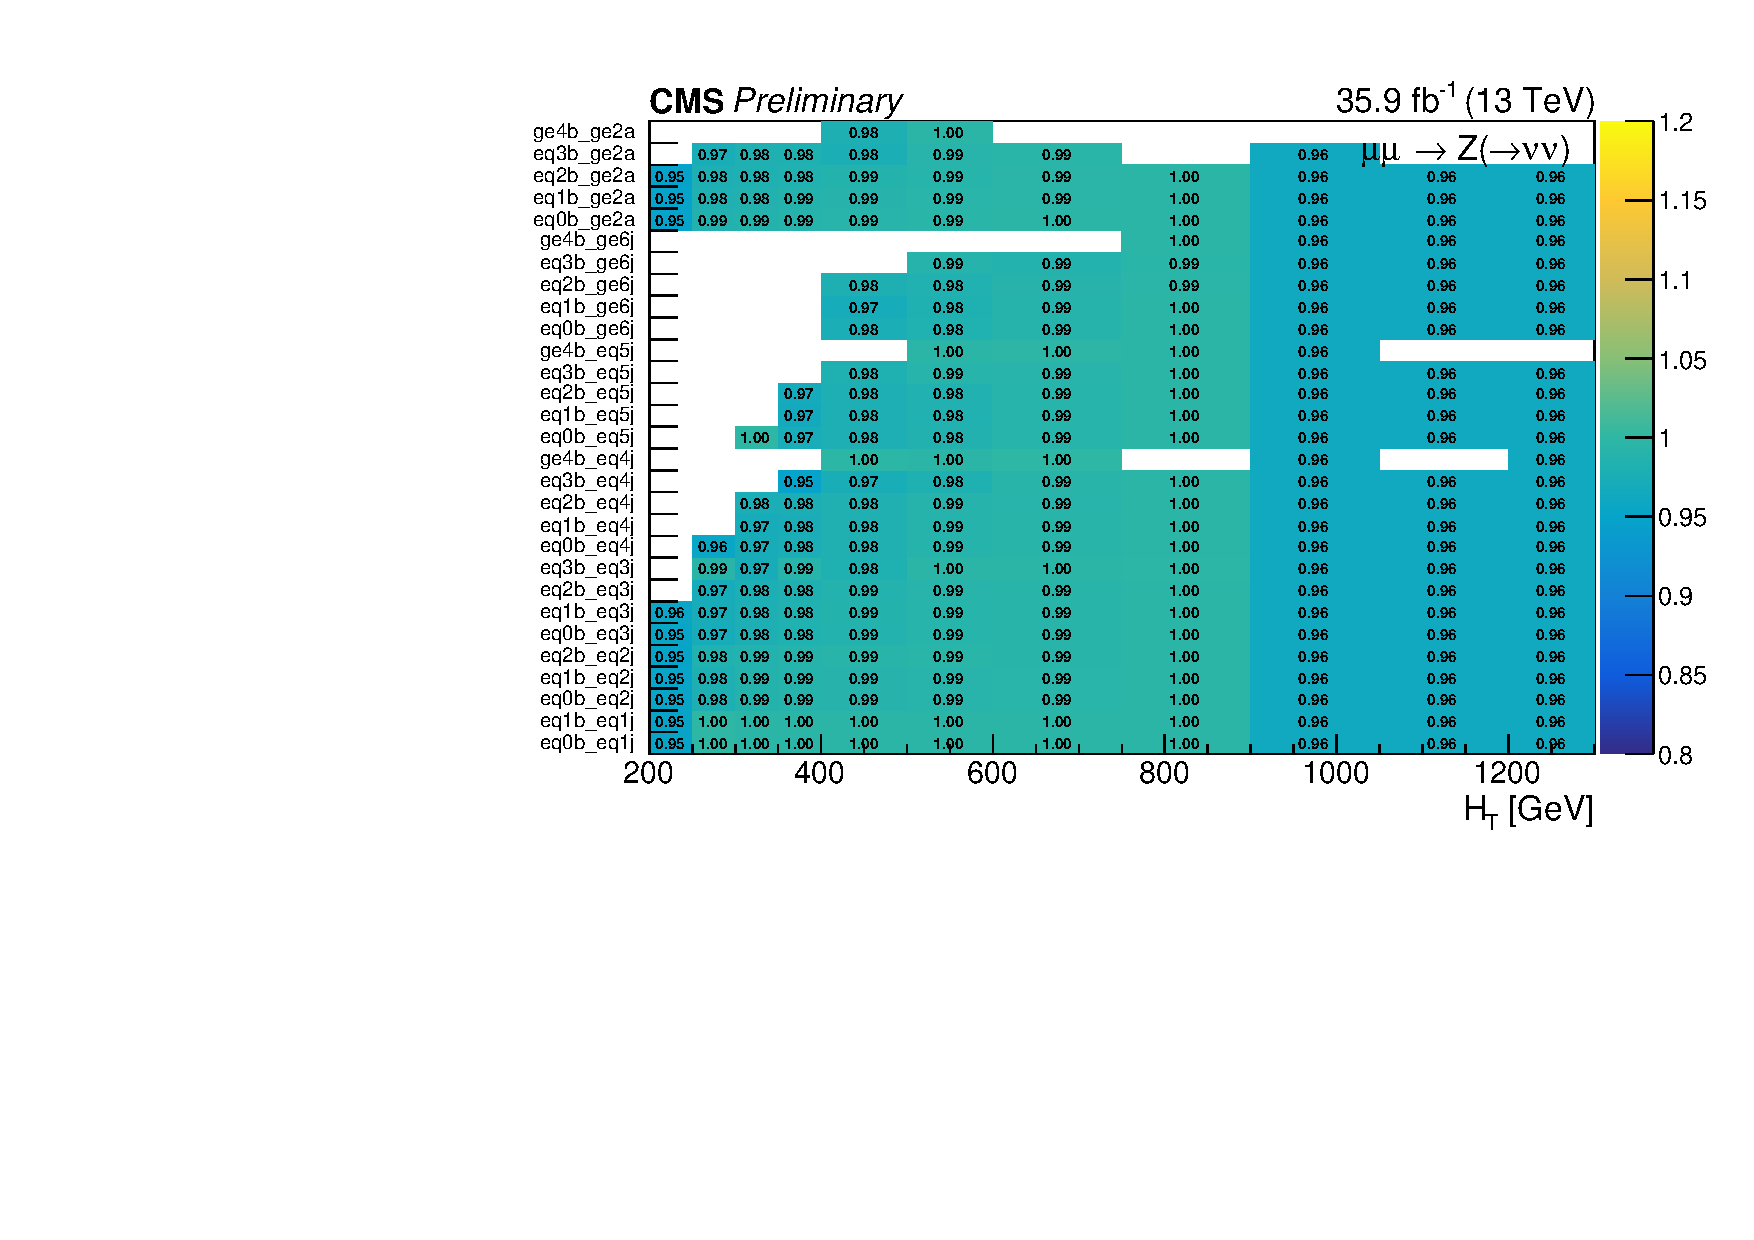
\includegraphics[width=0.5\textwidth]{figures/mcSystematics36p4fb/plots/tfratio_mumu_Zinv_2d_triggerWeightDown.pdf}
  }\\
  \subfigure[Up/down variations versus \njet.]{
    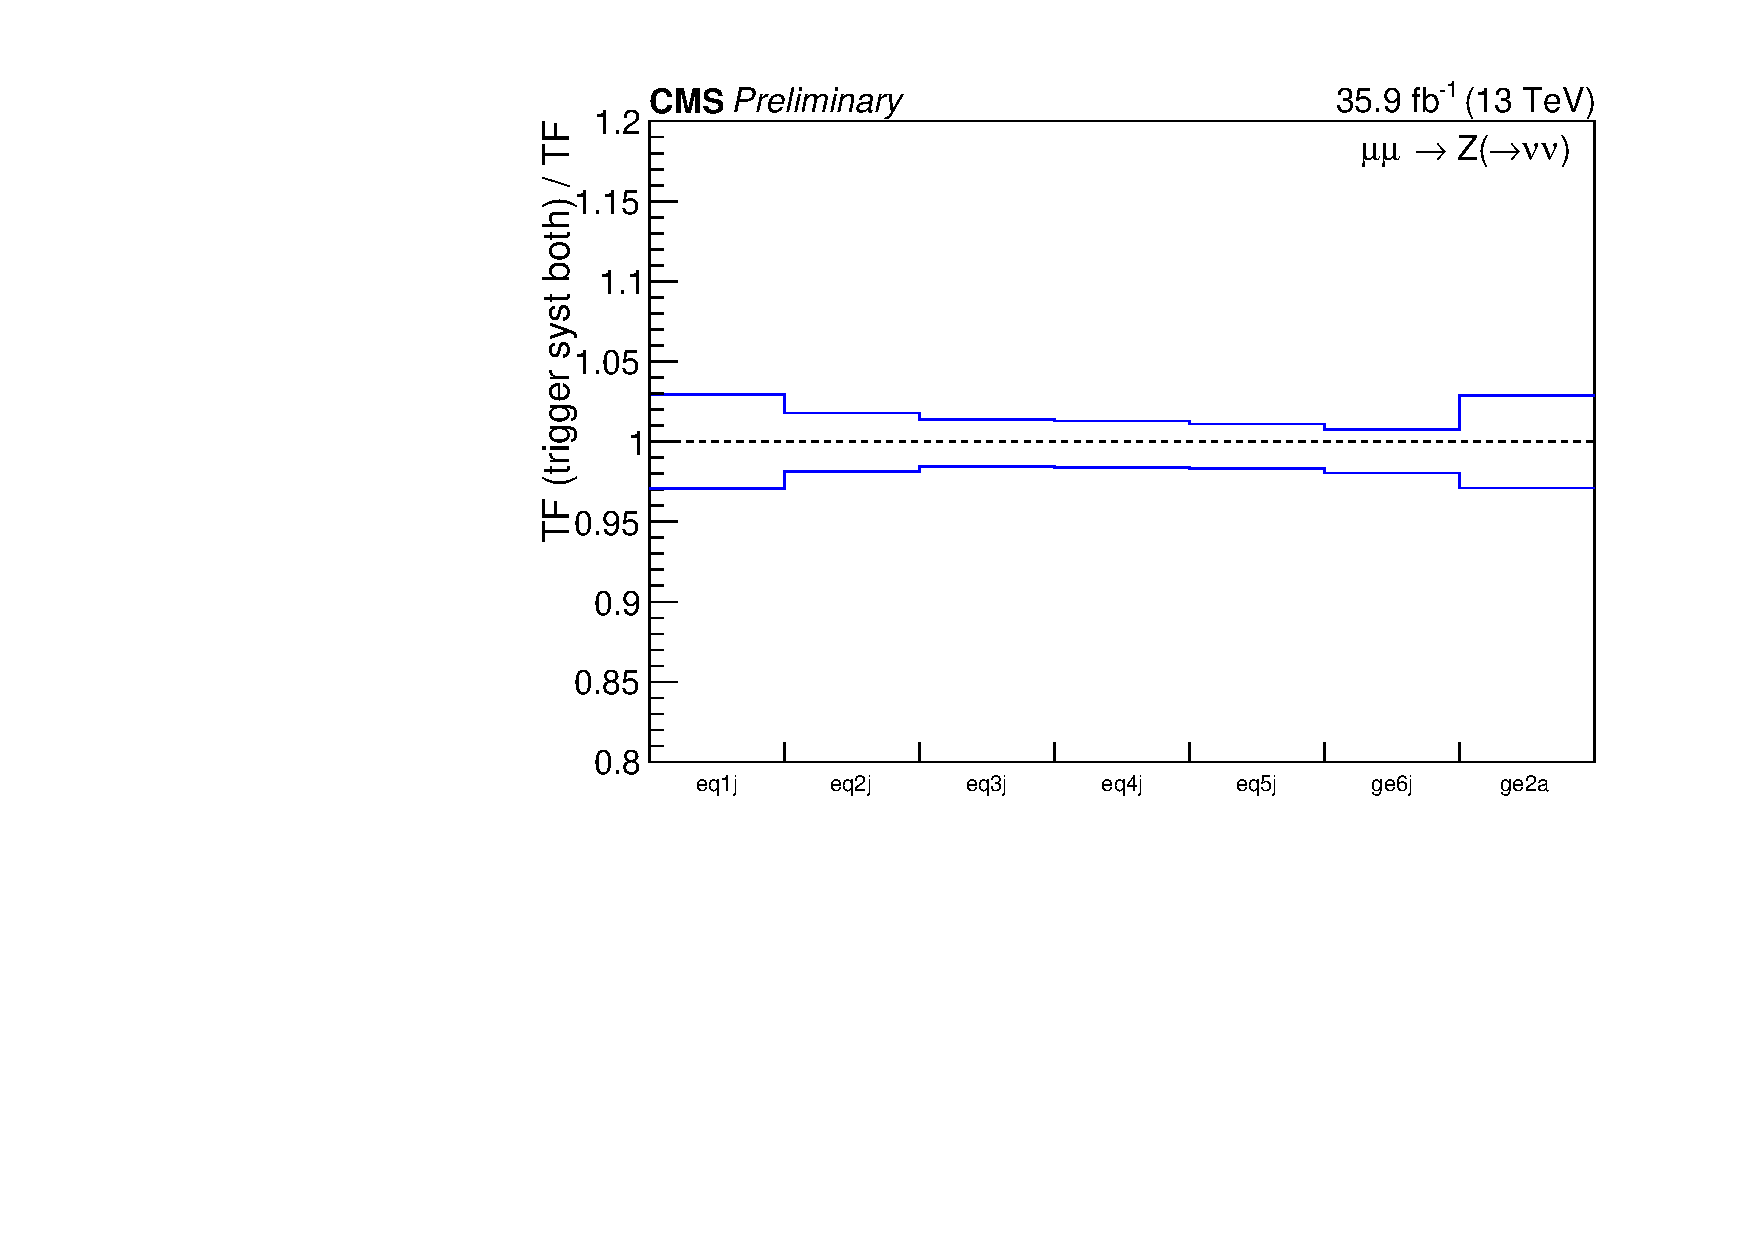
\includegraphics[width=0.5\textwidth]{figures/mcSystematics36p4fb/plots/tfratio_mumu_Zinv_njet_triggerWeightUp.pdf}
  } ~
  \subfigure[Up/down variations versus \scalht.]{
    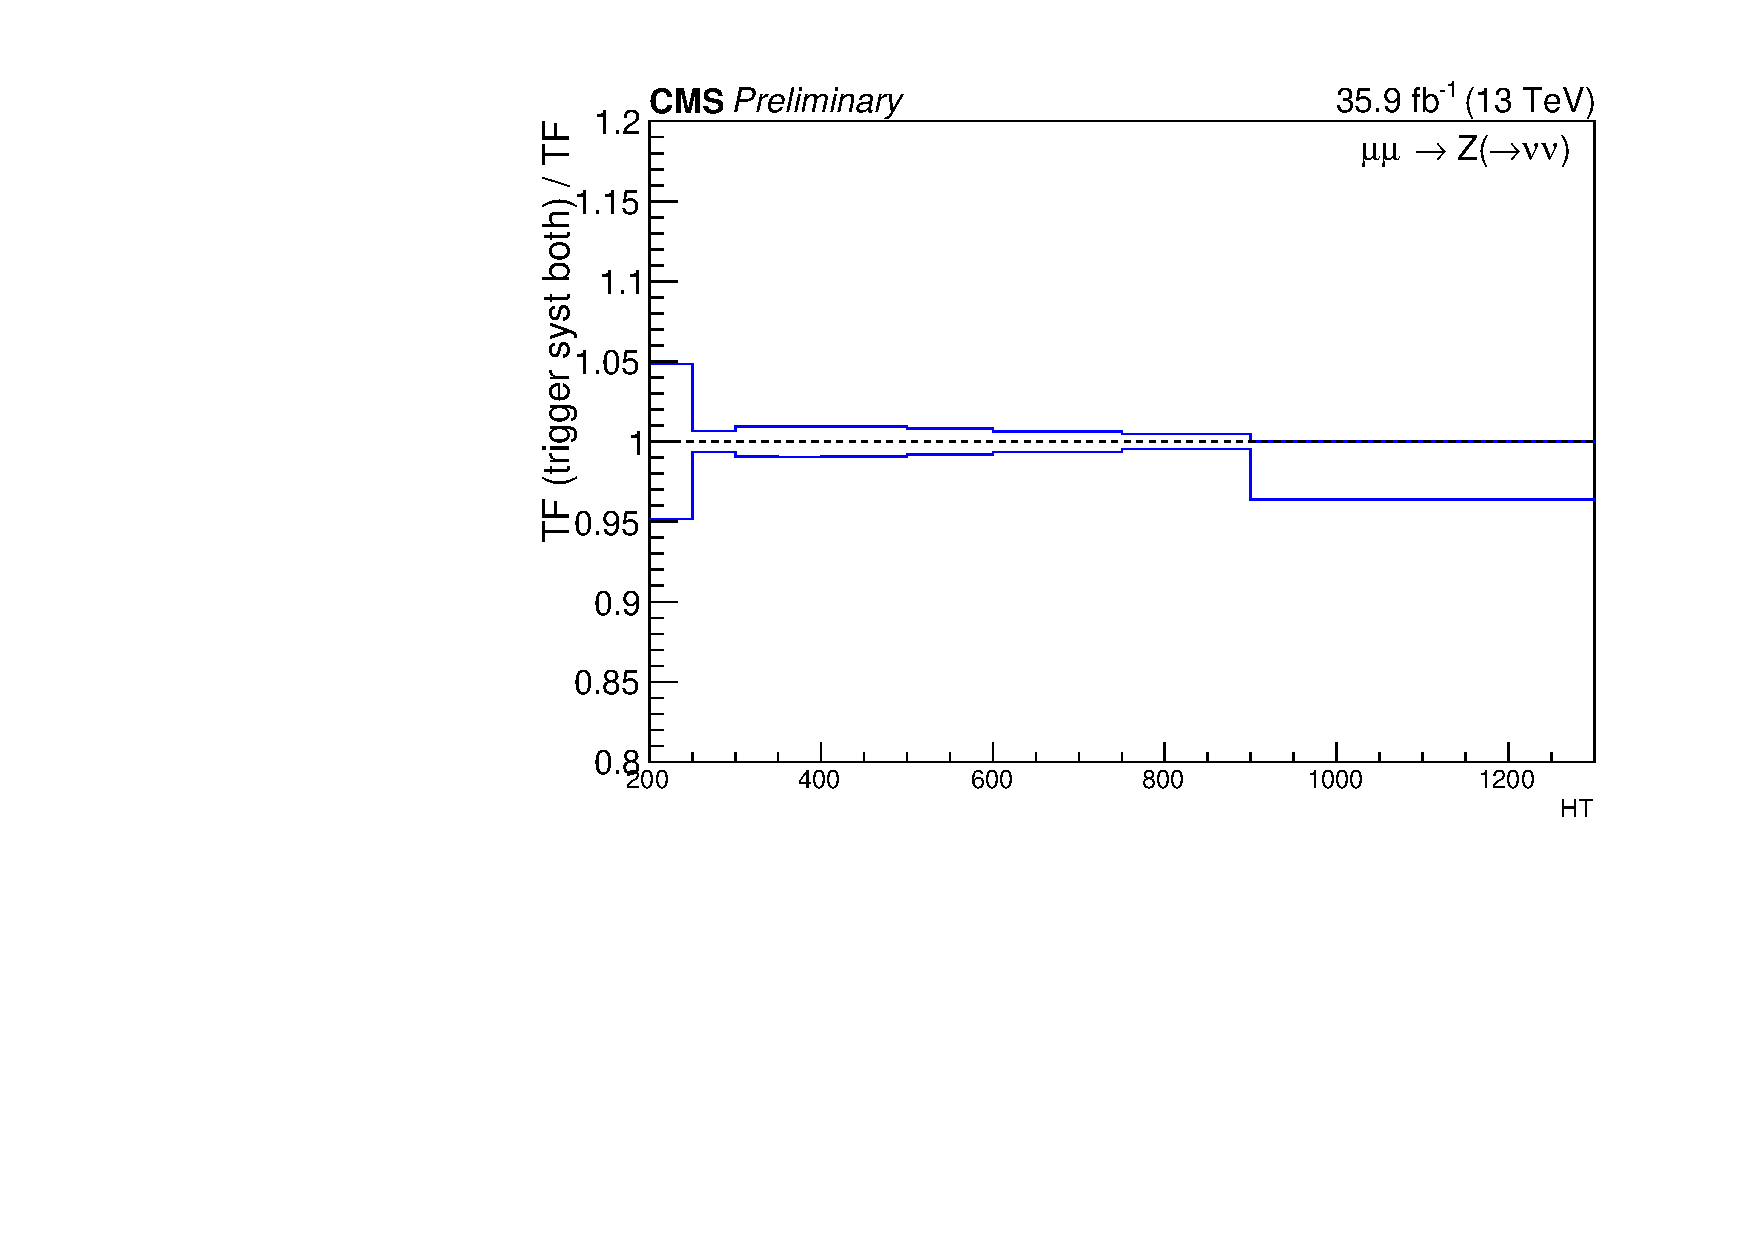
\includegraphics[width=0.5\textwidth]{figures/mcSystematics36p4fb/plots/tfratio_mumu_Zinv_ht_triggerWeightUp.pdf}
  } \\
  \subfigure[Up/down variations versus \nb.]{
    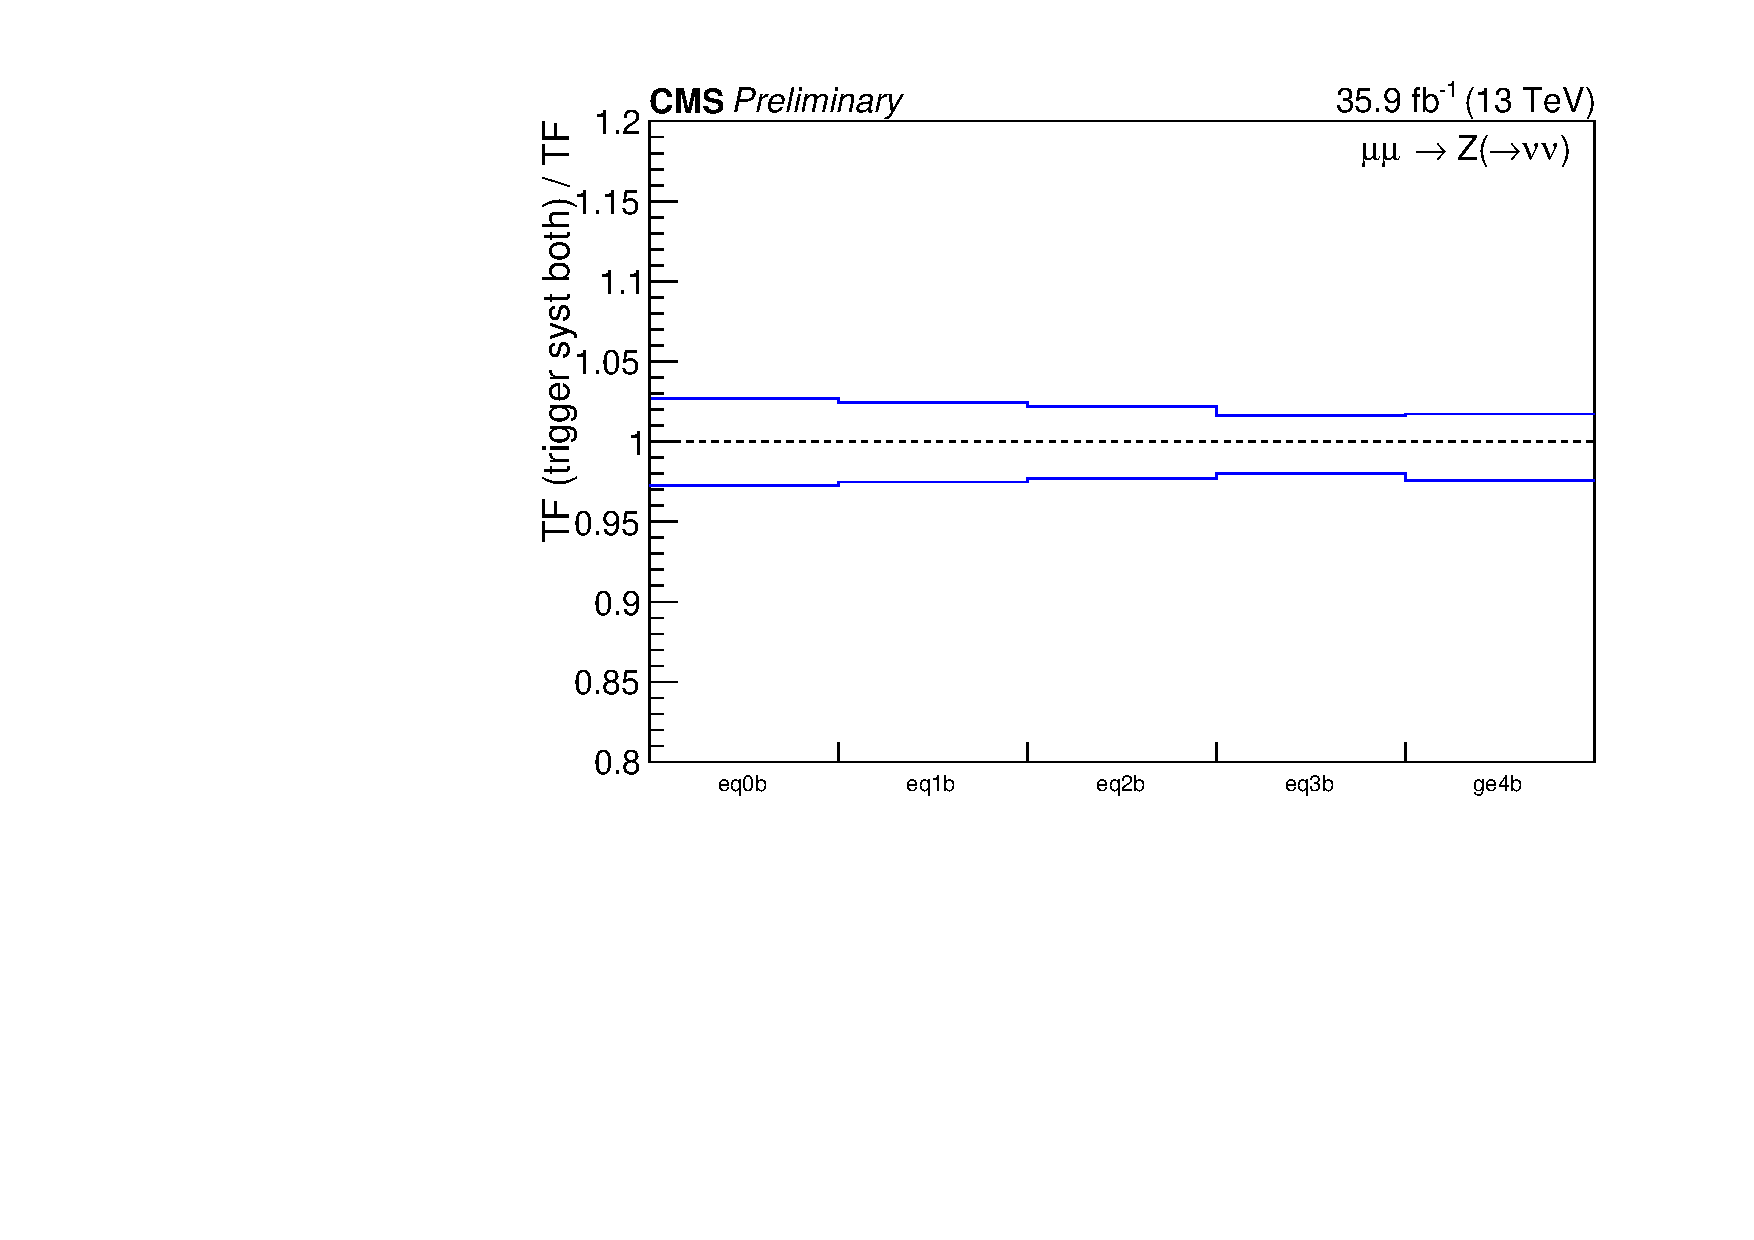
\includegraphics[width=0.5\textwidth]{figures/mcSystematics36p4fb/plots/tfratio_mumu_Zinv_bjet_triggerWeightUp.pdf}
  } ~
  \subfigure[Up/down variations versus \mht.]{
    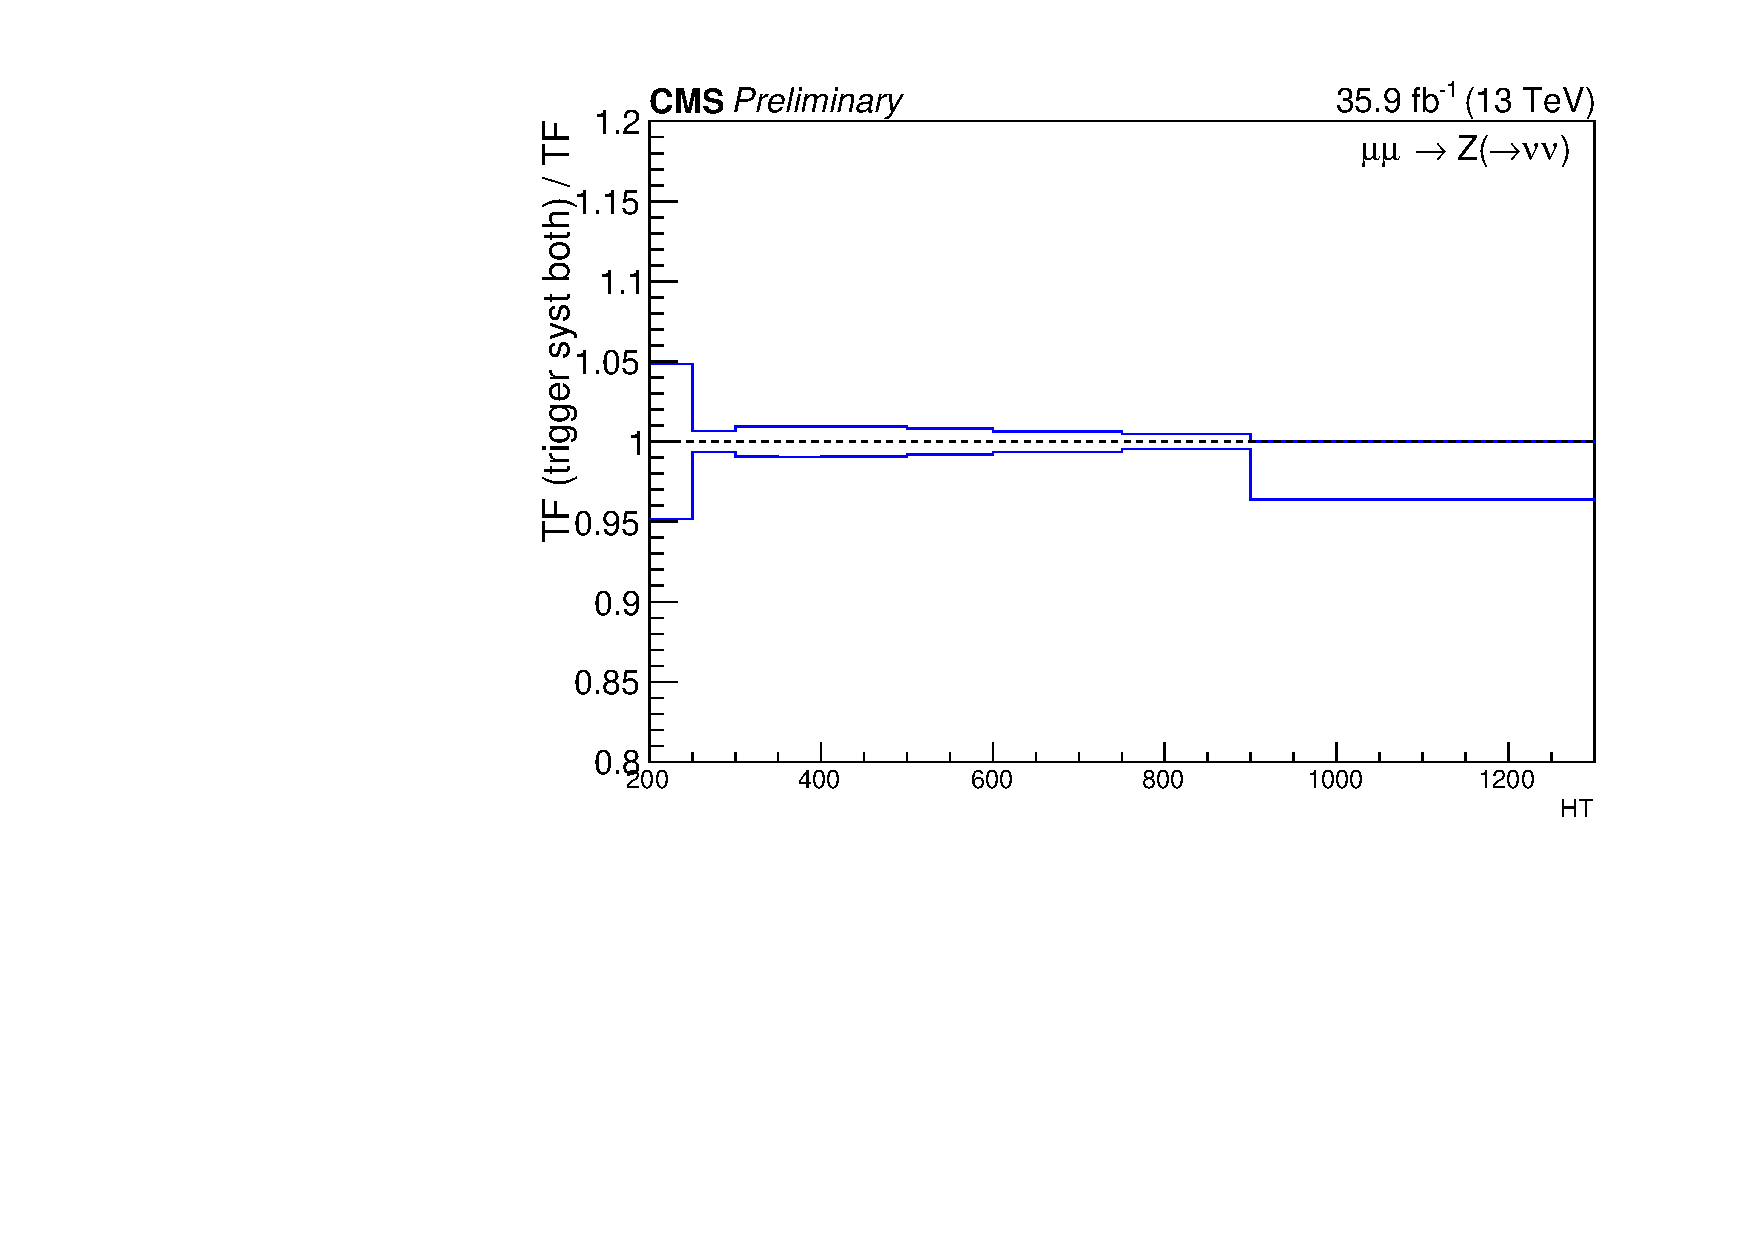
\includegraphics[width=0.5\textwidth]{figures/mcSystematics36p4fb/plots/tfratio_mumu_Zinv_ht_triggerWeightUp.pdf}
  } \\
  \caption{\label{fig:tfSyst_trigger_mumuToZinv} The relative change in the
    ``$\mmj \rightarrow \znunu\ + \textrm{jets}$'' transfer factors from
    simulation due to $\pm1\sigma$ uncertainties in the signal trigger
    efficiencies.  }
\end{figure}

\clearpage
\subsection{Lepton trigger / identification / isolation efficiencies}

\begin{figure}[!h]
  \centering
  \subfigure[Up variation versus (\njet,\nb) category and \scalht.]{
    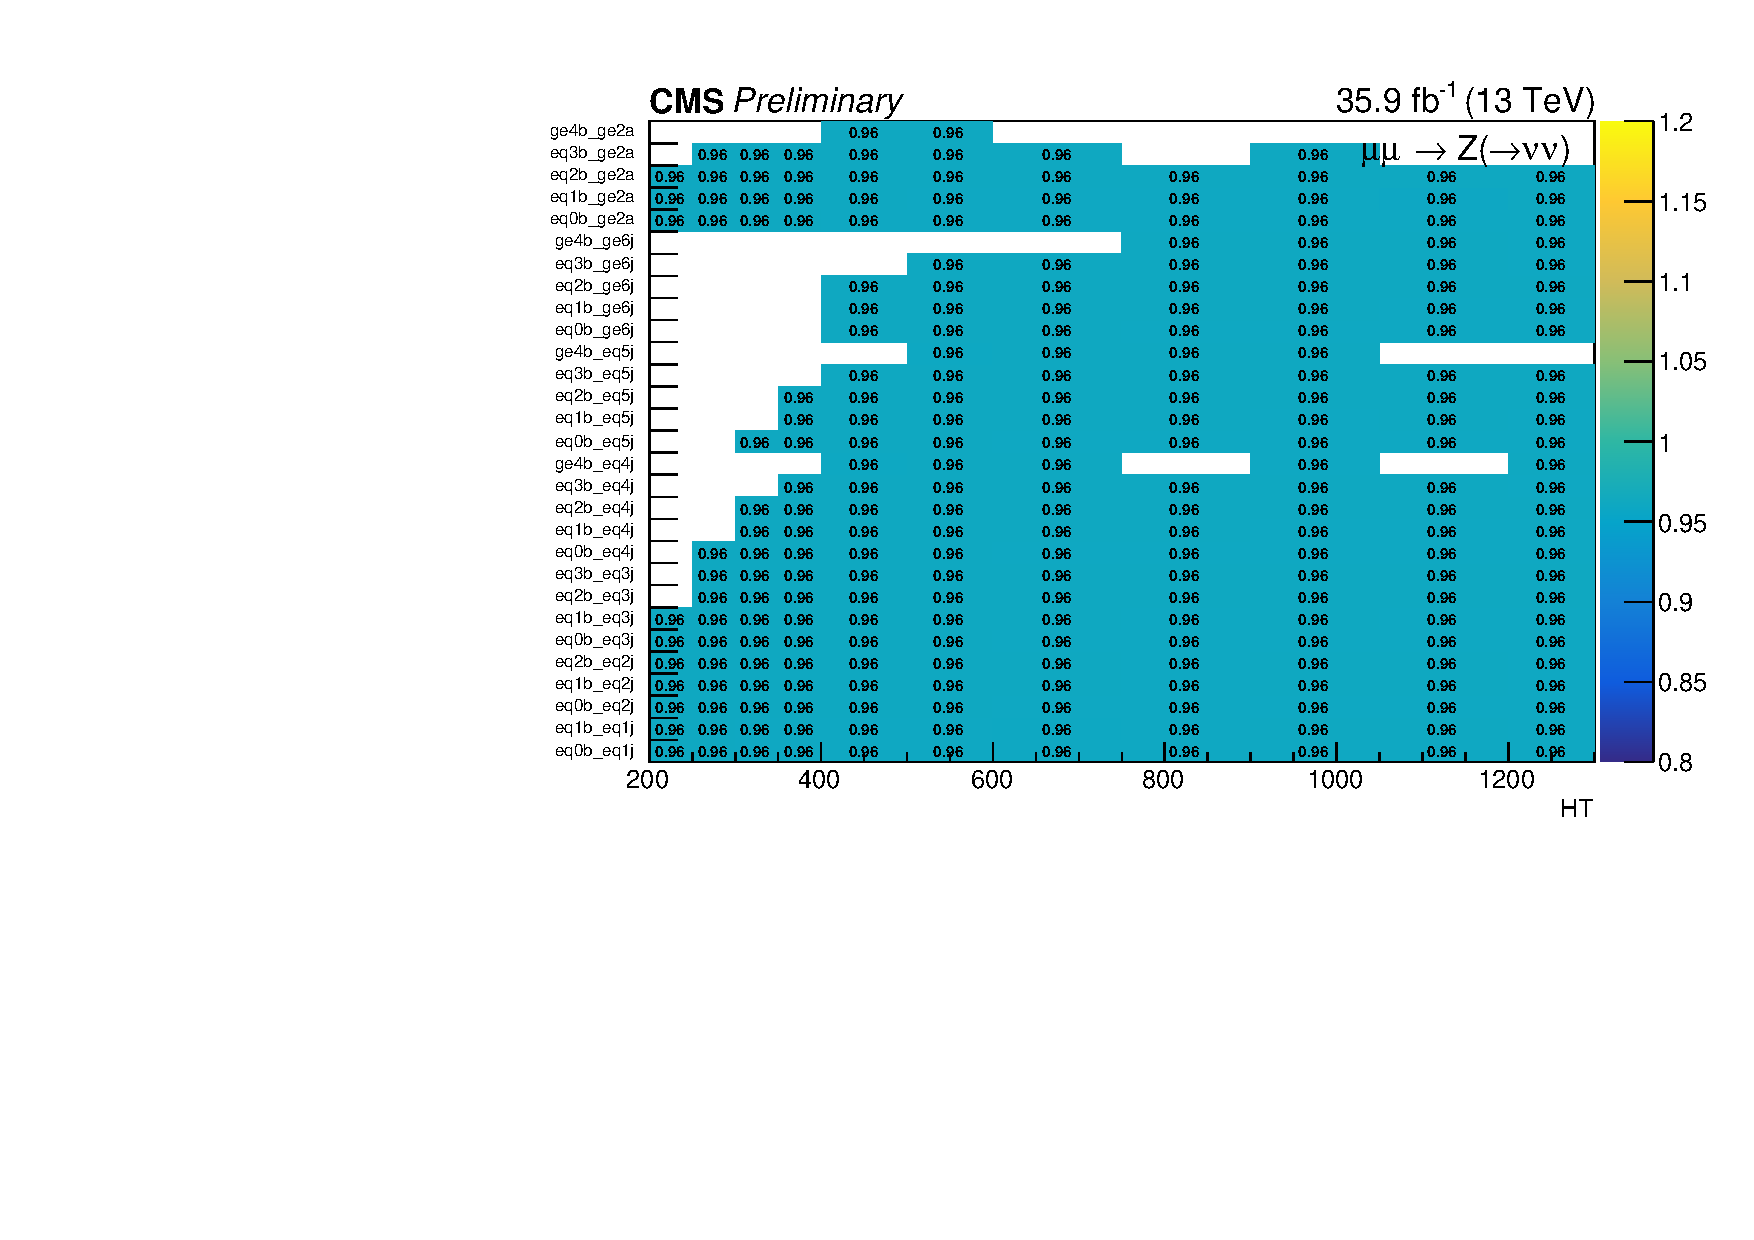
\includegraphics[width=0.5\textwidth]{figures/mcSystematics36p4fb/plots/tfratio_mumu_Zinv_2d_muonSfWeightUp.pdf}
  } ~
  \subfigure[Down variation versus (\njet,\nb) category and \scalht.]{
    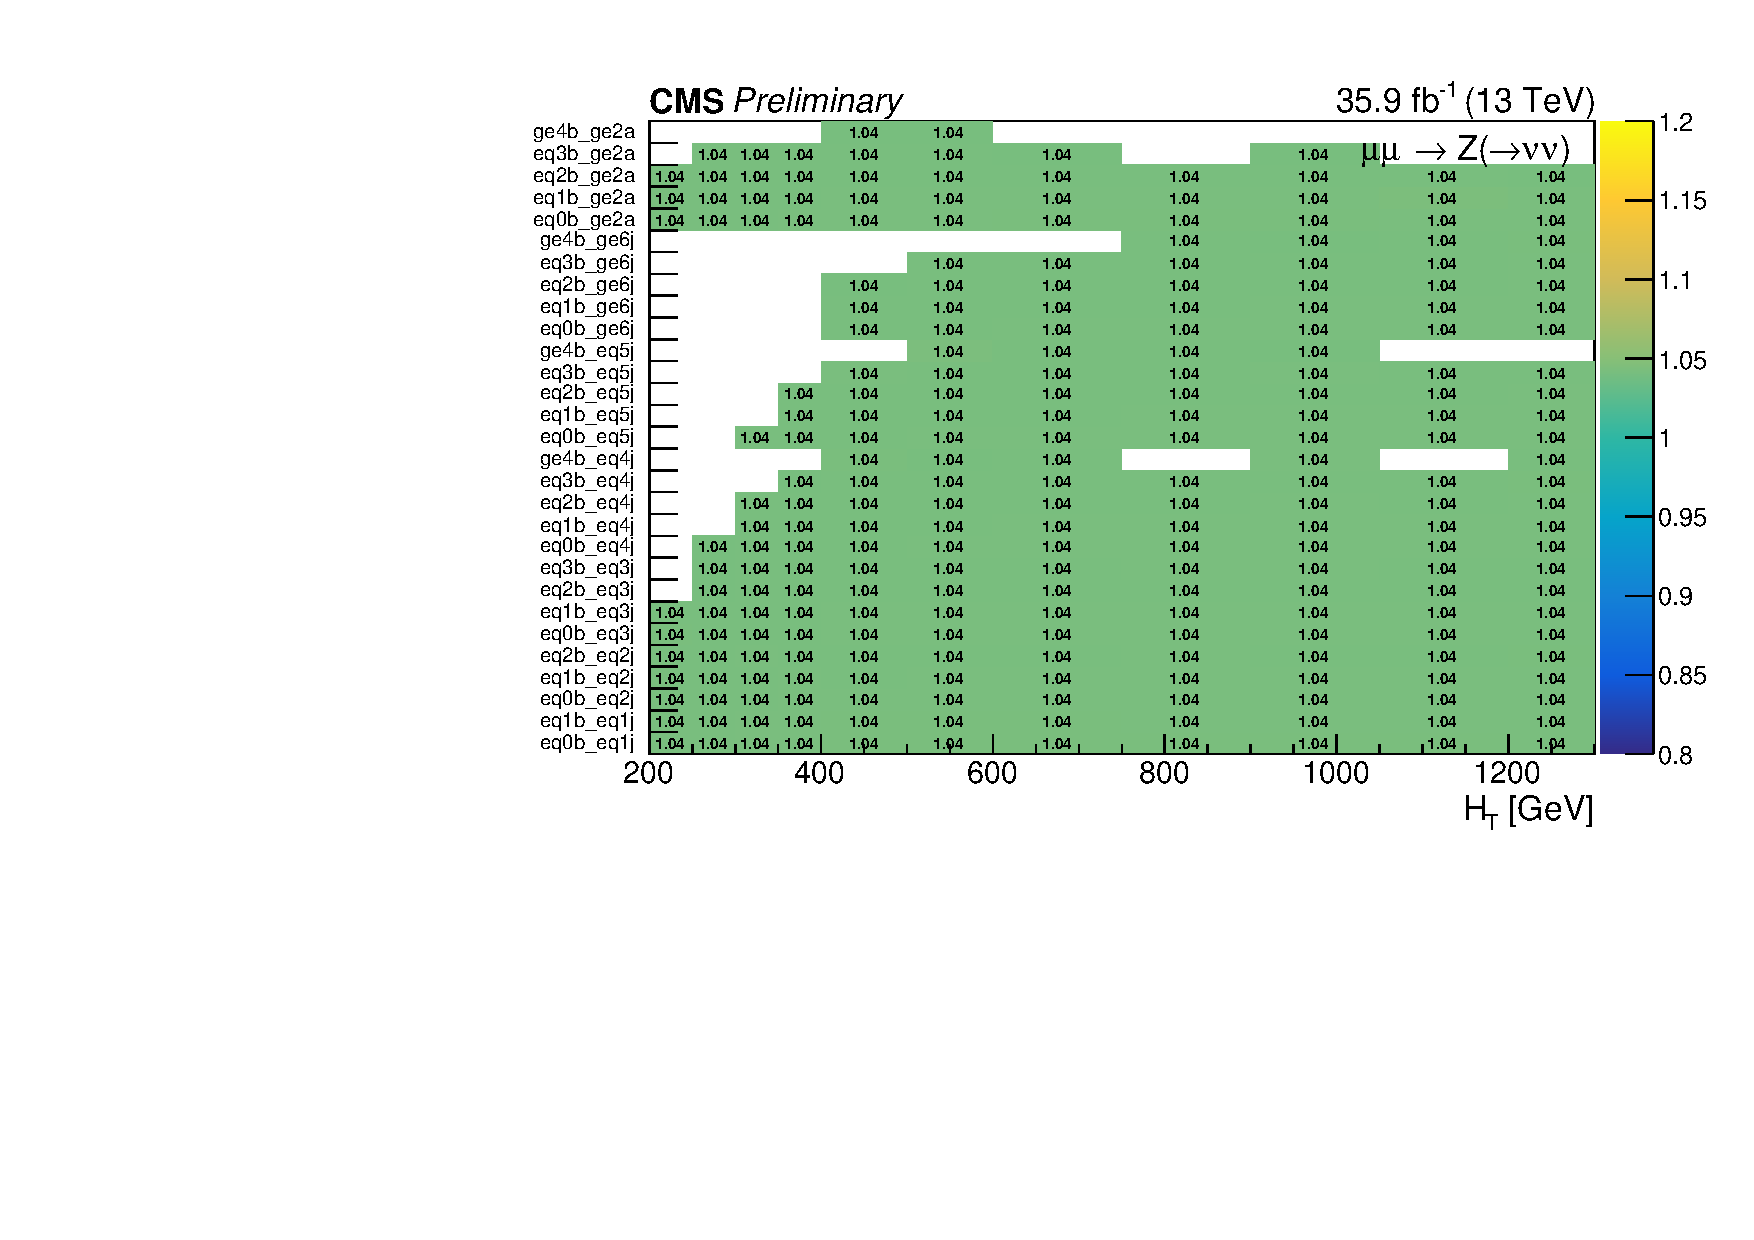
\includegraphics[width=0.5\textwidth]{figures/mcSystematics36p4fb/plots/tfratio_mumu_Zinv_2d_muonSfWeightDown.pdf}
  }\\
  \subfigure[Up/down variations versus \njet.]{
    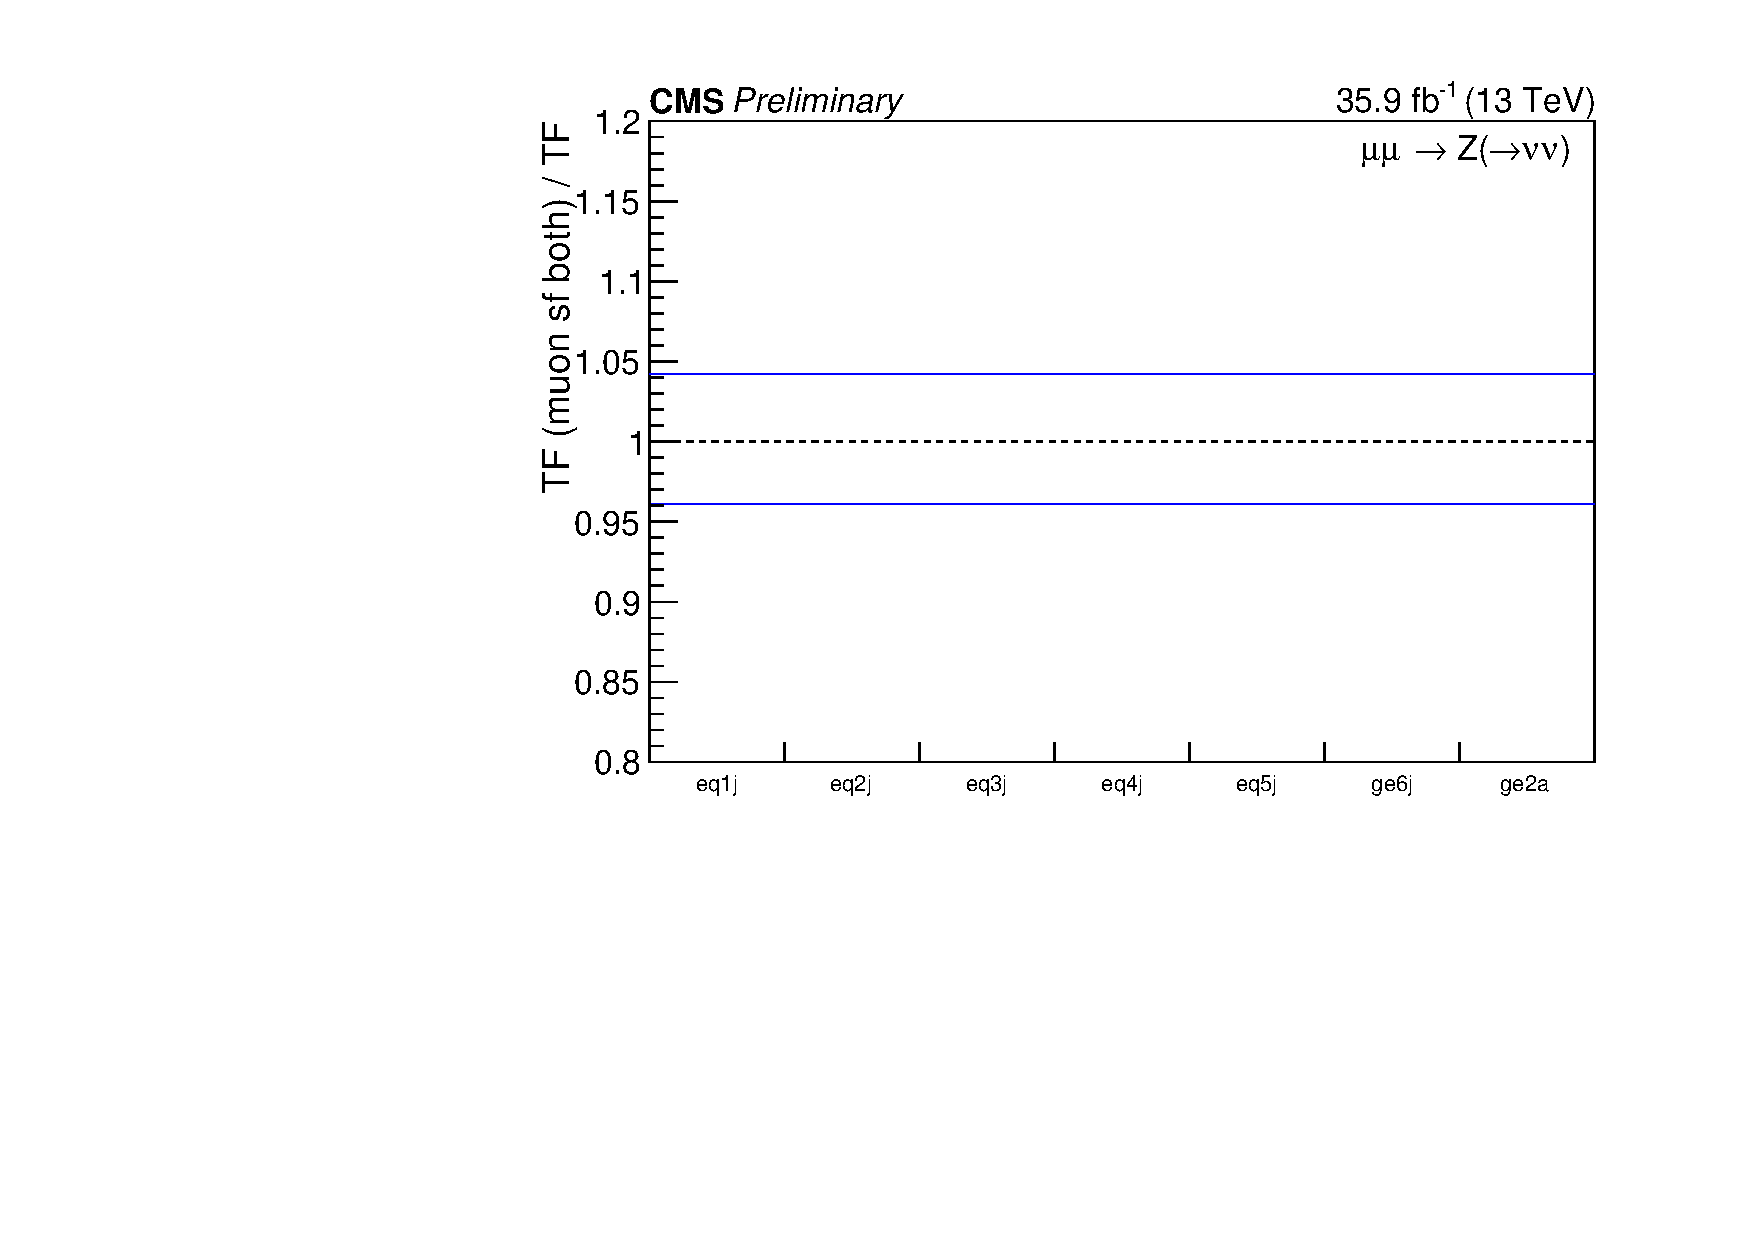
\includegraphics[width=0.5\textwidth]{figures/mcSystematics36p4fb/plots/tfratio_mumu_Zinv_njet_muonSfWeightUp.pdf}
  } ~
  \subfigure[Up/down variations versus \scalht.]{
    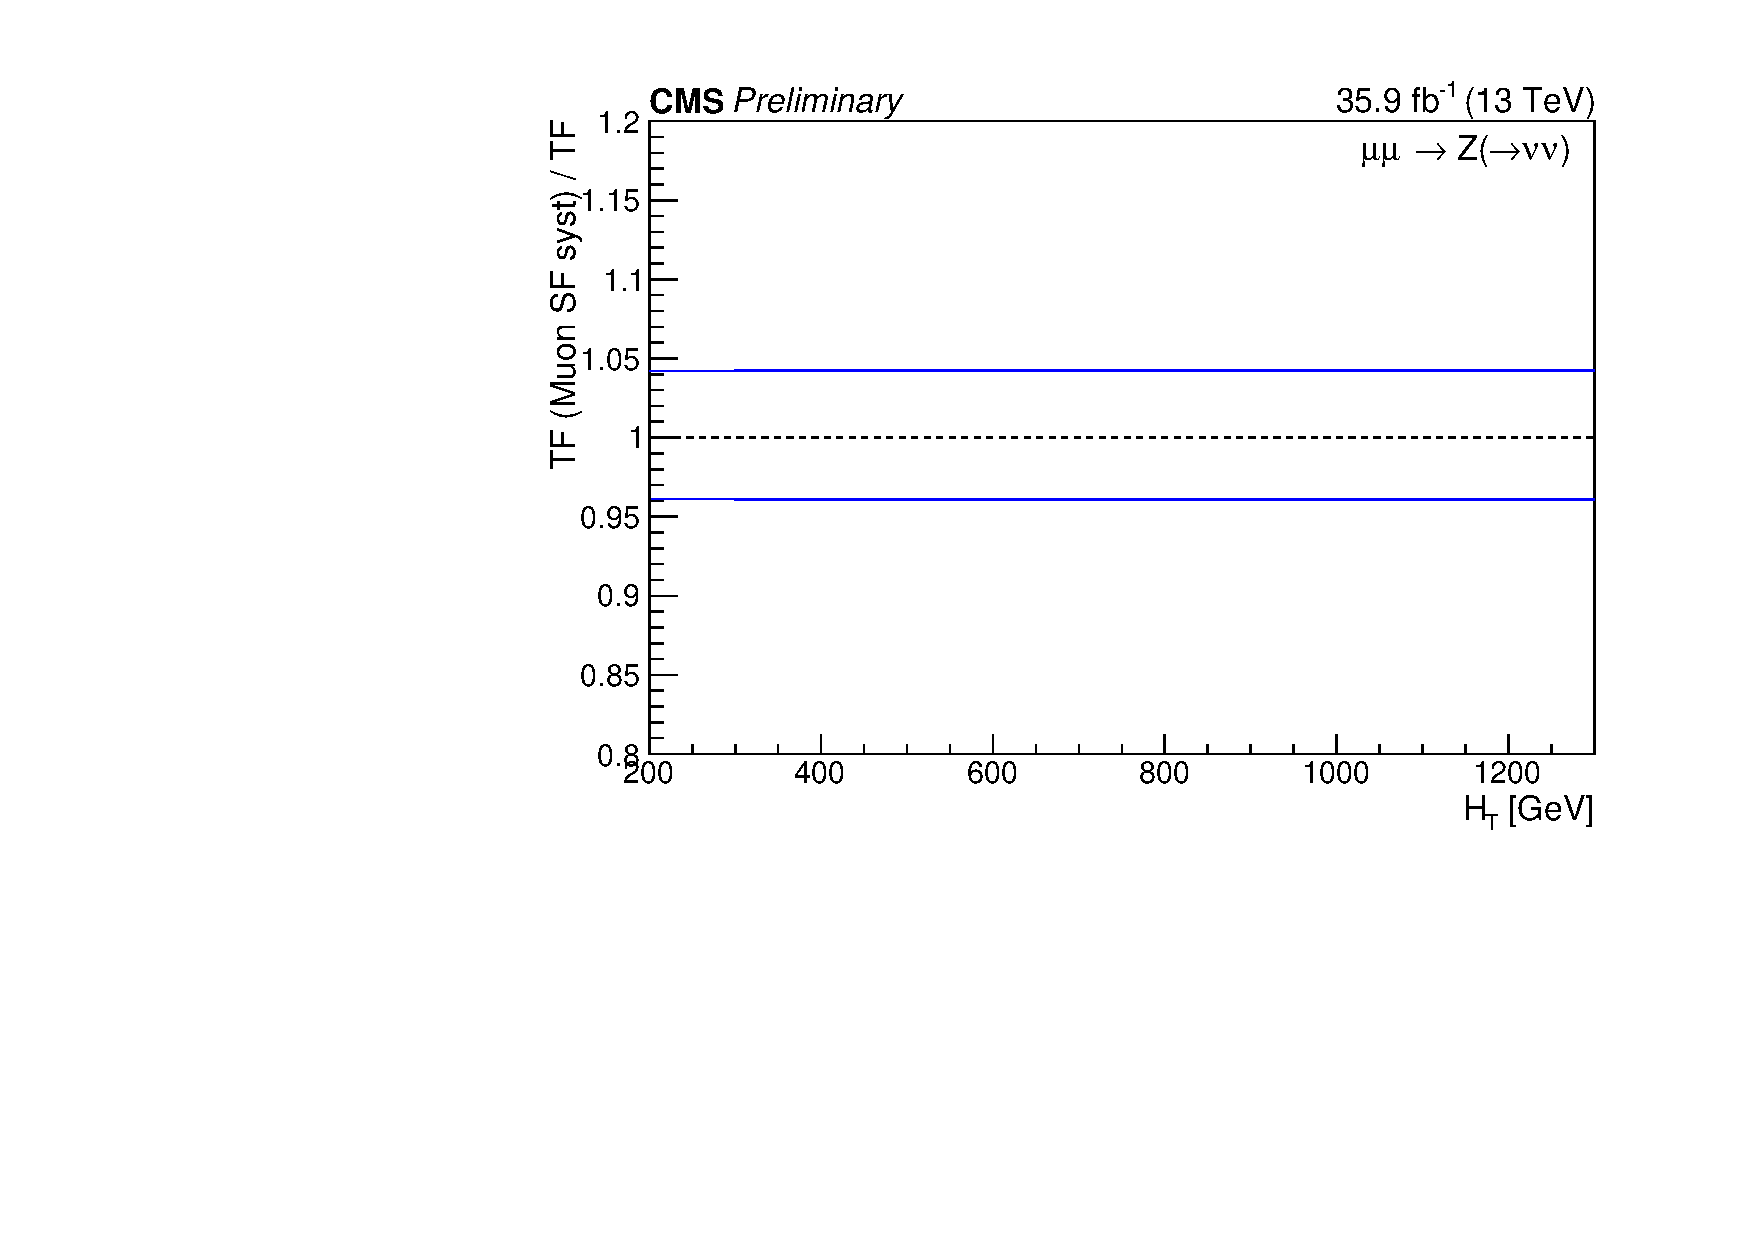
\includegraphics[width=0.5\textwidth]{figures/mcSystematics36p4fb/plots/tfratio_mumu_Zinv_ht_muonSfWeightUp.pdf}
  } \\
  \subfigure[Up/down variations versus \nb.]{
    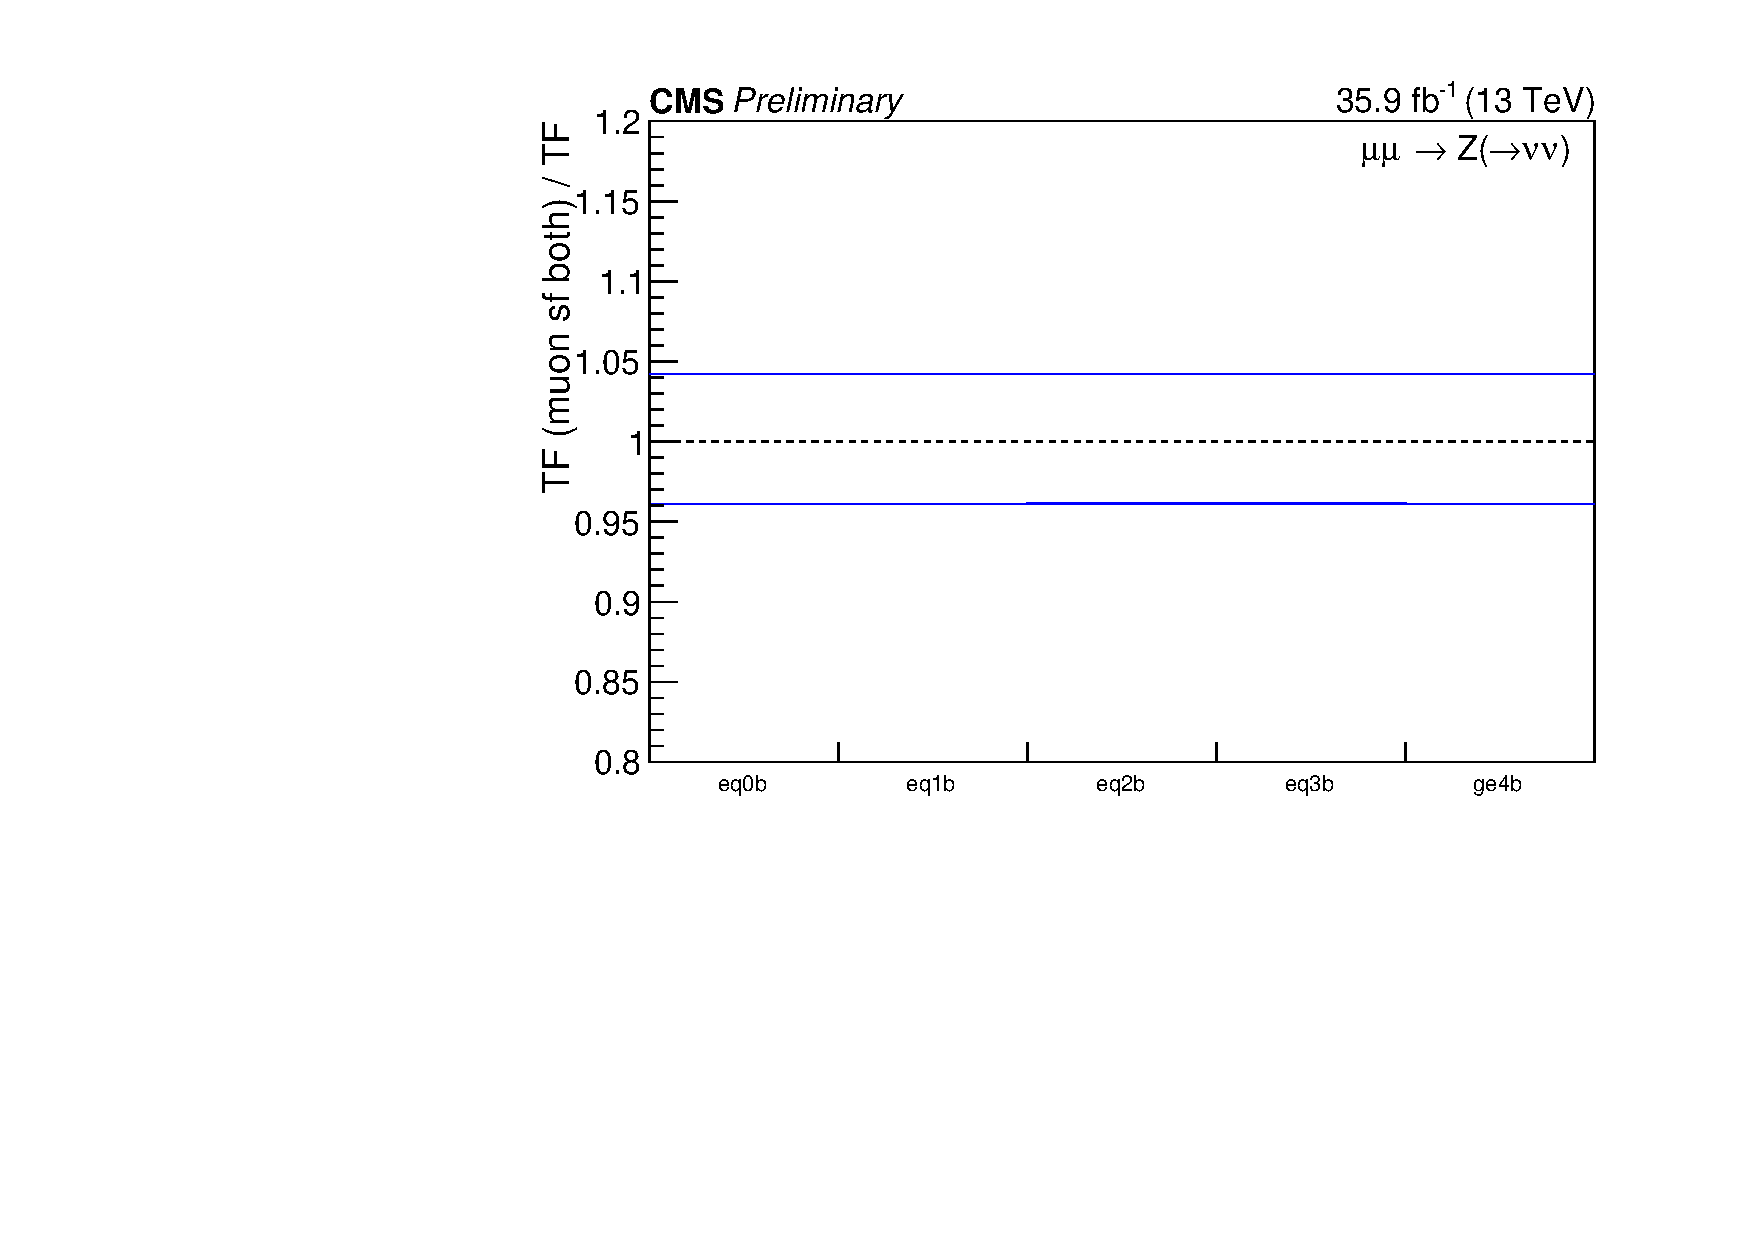
\includegraphics[width=0.5\textwidth]{figures/mcSystematics36p4fb/plots/tfratio_mumu_Zinv_bjet_muonSfWeightUp.pdf}
  } ~
  \subfigure[Up/down variations versus \mht.]{
    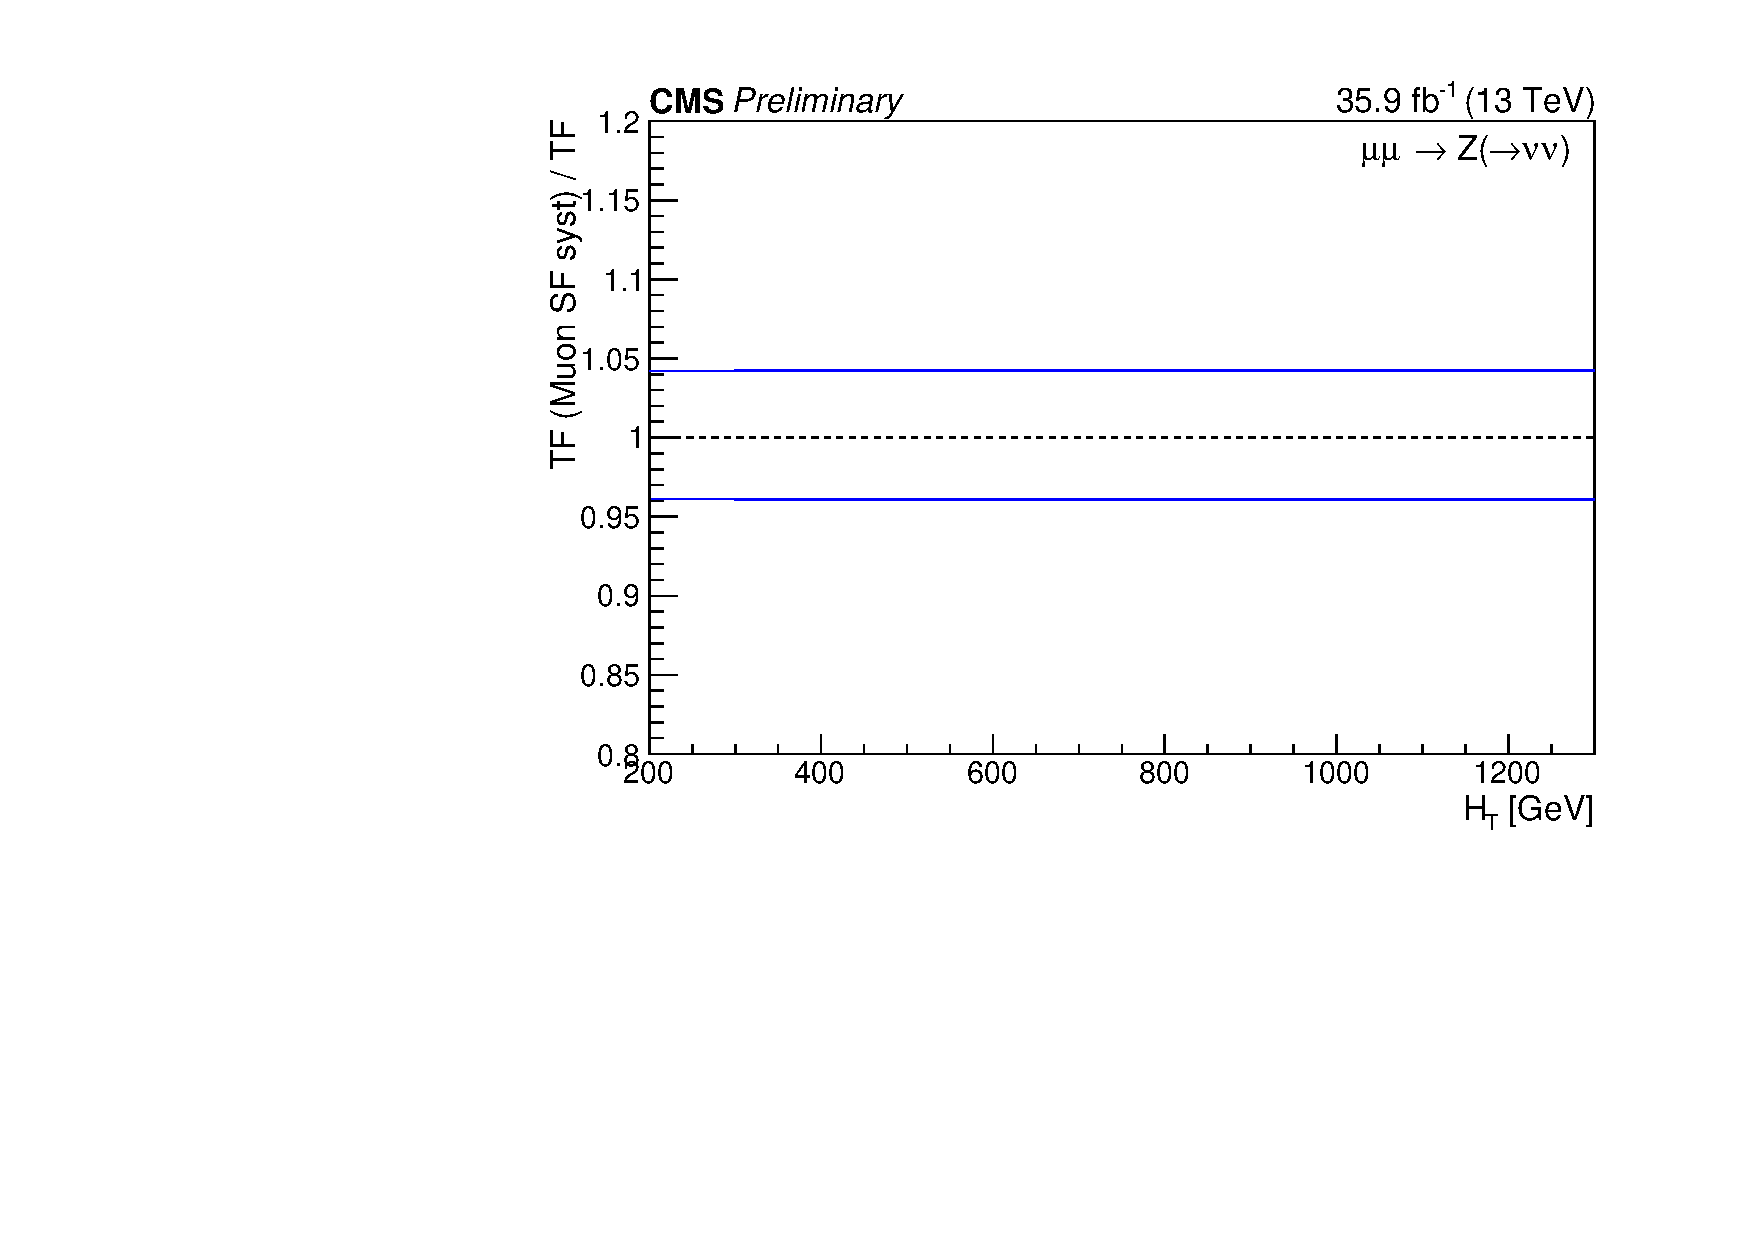
\includegraphics[width=0.5\textwidth]{figures/mcSystematics36p4fb/plots/tfratio_mumu_Zinv_ht_muonSfWeightUp.pdf}
  } \\
  \caption{\label{fig:tfSyst_muonsf_mumuToZinv} The relative change in the
    ``$\mmj \rightarrow \znunu\ + \textrm{jets}$'' transfer factors from
    simulation due to $\pm1\sigma$ uncertainties in efficiencies
    related to muon trigger, identification, and isolation.  }
\end{figure}

\clearpage
\begin{figure}[!h]
  \centering
  \subfigure[Up variation versus (\njet,\nb) category and \scalht.]{
    \includegraphics[width=0.5\textwidth]{figures/mcSystematics36p4fb/plots/tfratio_mumu_Zinv_2d_leptonVetoSystFullSimWeightUp.pdf}
  } ~
  \subfigure[Down variation versus (\njet,\nb) category and \scalht.]{
    \includegraphics[width=0.5\textwidth]{figures/mcSystematics36p4fb/plots/tfratio_mumu_Zinv_2d_leptonVetoSystFullSimWeightDown.pdf}
  }\\
  \subfigure[Up/down variations versus \njet.]{
    \includegraphics[width=0.5\textwidth]{figures/mcSystematics36p4fb/plots/tfratio_mumu_Zinv_njet_leptonVetoSystFullSimWeightUp.pdf}
  } ~
  \subfigure[Up/down variations versus \scalht.]{
    \includegraphics[width=0.5\textwidth]{figures/mcSystematics36p4fb/plots/tfratio_mumu_Zinv_ht_leptonVetoSystFullSimWeightUp.pdf}
  } \\
  \subfigure[Up/down variations versus \nb.]{
    \includegraphics[width=0.5\textwidth]{figures/mcSystematics36p4fb/plots/tfratio_mumu_Zinv_bjet_leptonVetoSystFullSimWeightUp.pdf}
  } ~
  \subfigure[Up/down variations versus \mht.]{
    \includegraphics[width=0.5\textwidth]{figures/mcSystematics36p4fb/plots/tfratio_mumu_Zinv_ht_leptonVetoSystFullSimWeightUp.pdf}
  } \\
  \caption{\label{fig:tfSyst_leptonveto_mumuToZinv} The relative change in the
    ``$\mmj \rightarrow \znunu\ + \textrm{jets}$'' transfer factors from
    simulation due to $\pm1\sigma$ uncertainties in the efficiency
    with which leptons are vetoed for the signal region.  }
\end{figure}

\clearpage
\subsection{Jet energy scale}

\begin{figure}[!h]
  \centering
  \subfigure[Up variation versus (\njet,\nb) category and \scalht.]{
    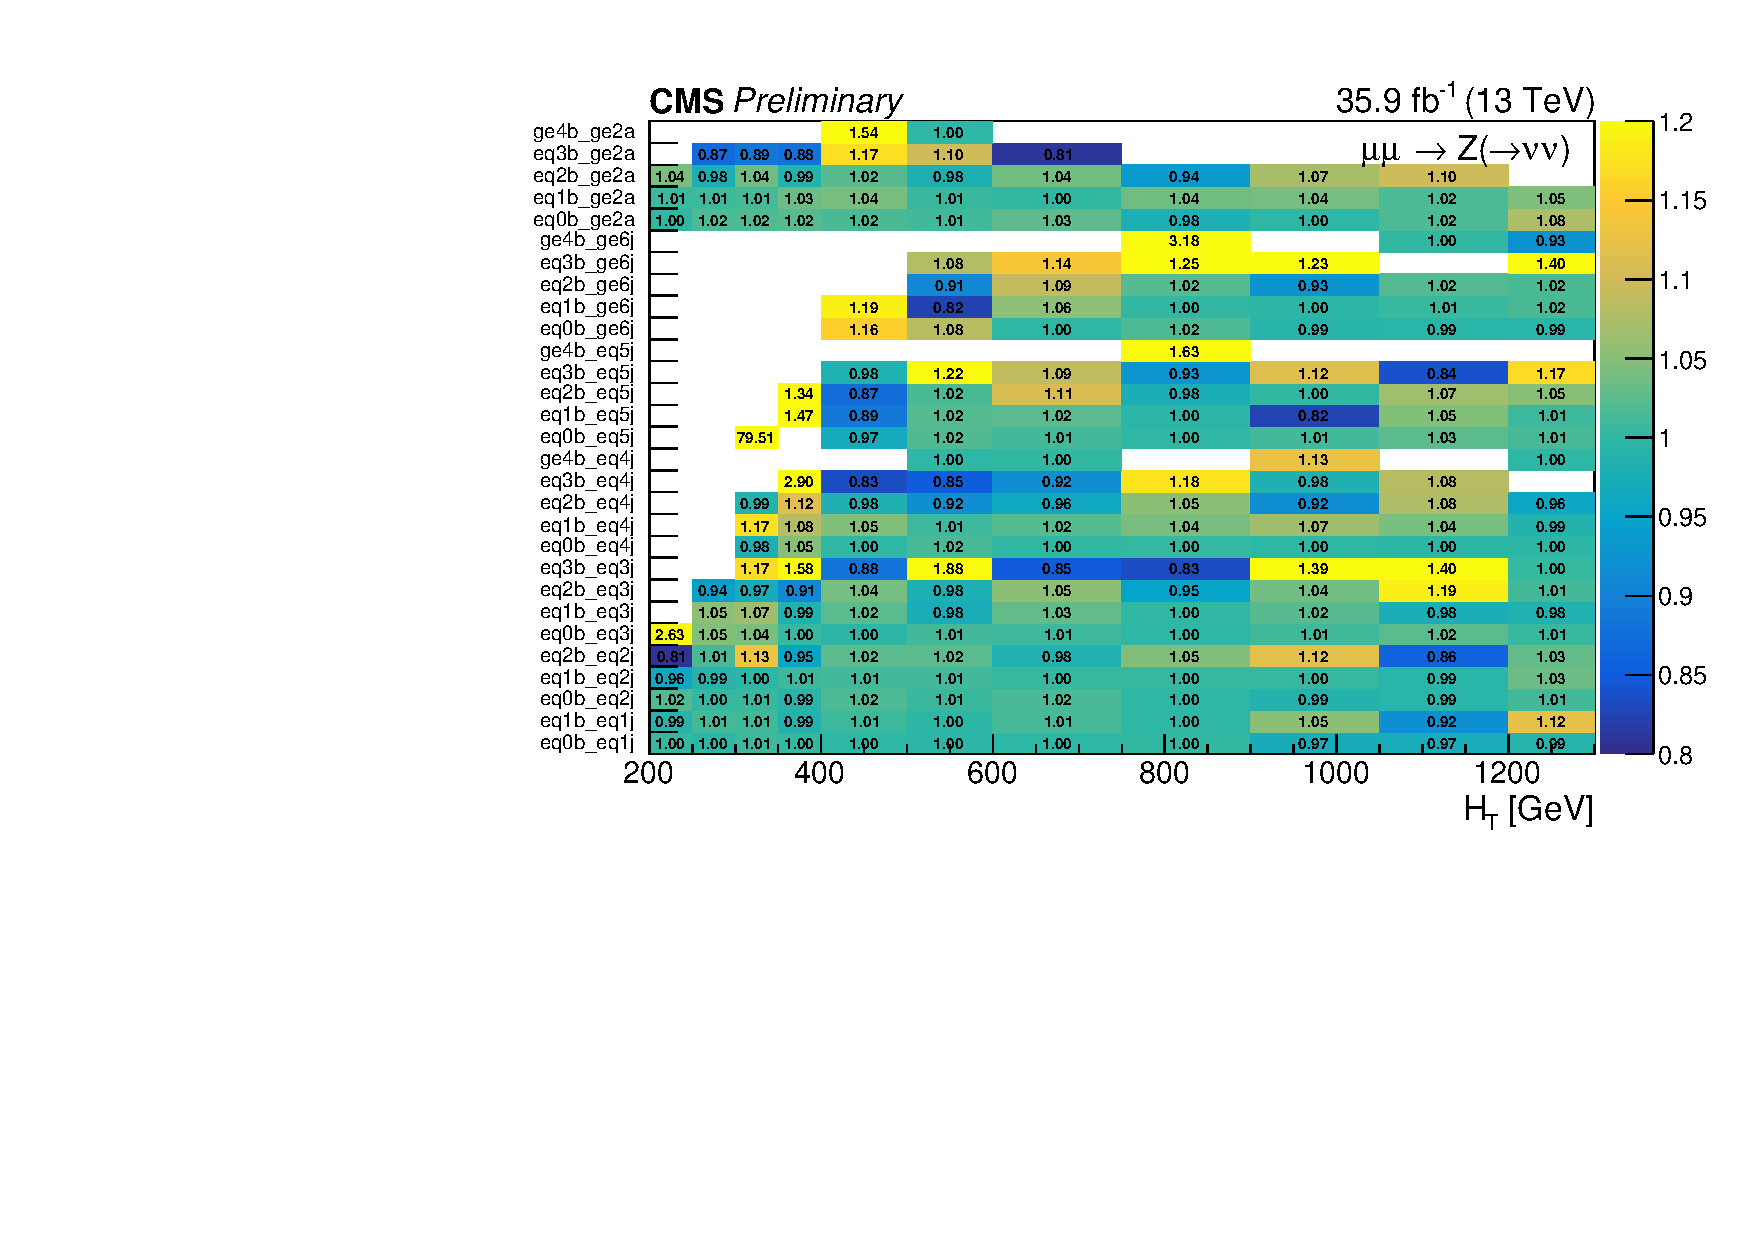
\includegraphics[width=0.5\textwidth]{figures/mcSystematics36p4fb/plots/tfratio_mumu_Zinv_2d_jecUp.pdf}
  } ~
  \subfigure[Down variation versus (\njet,\nb) category and \scalht.]{
    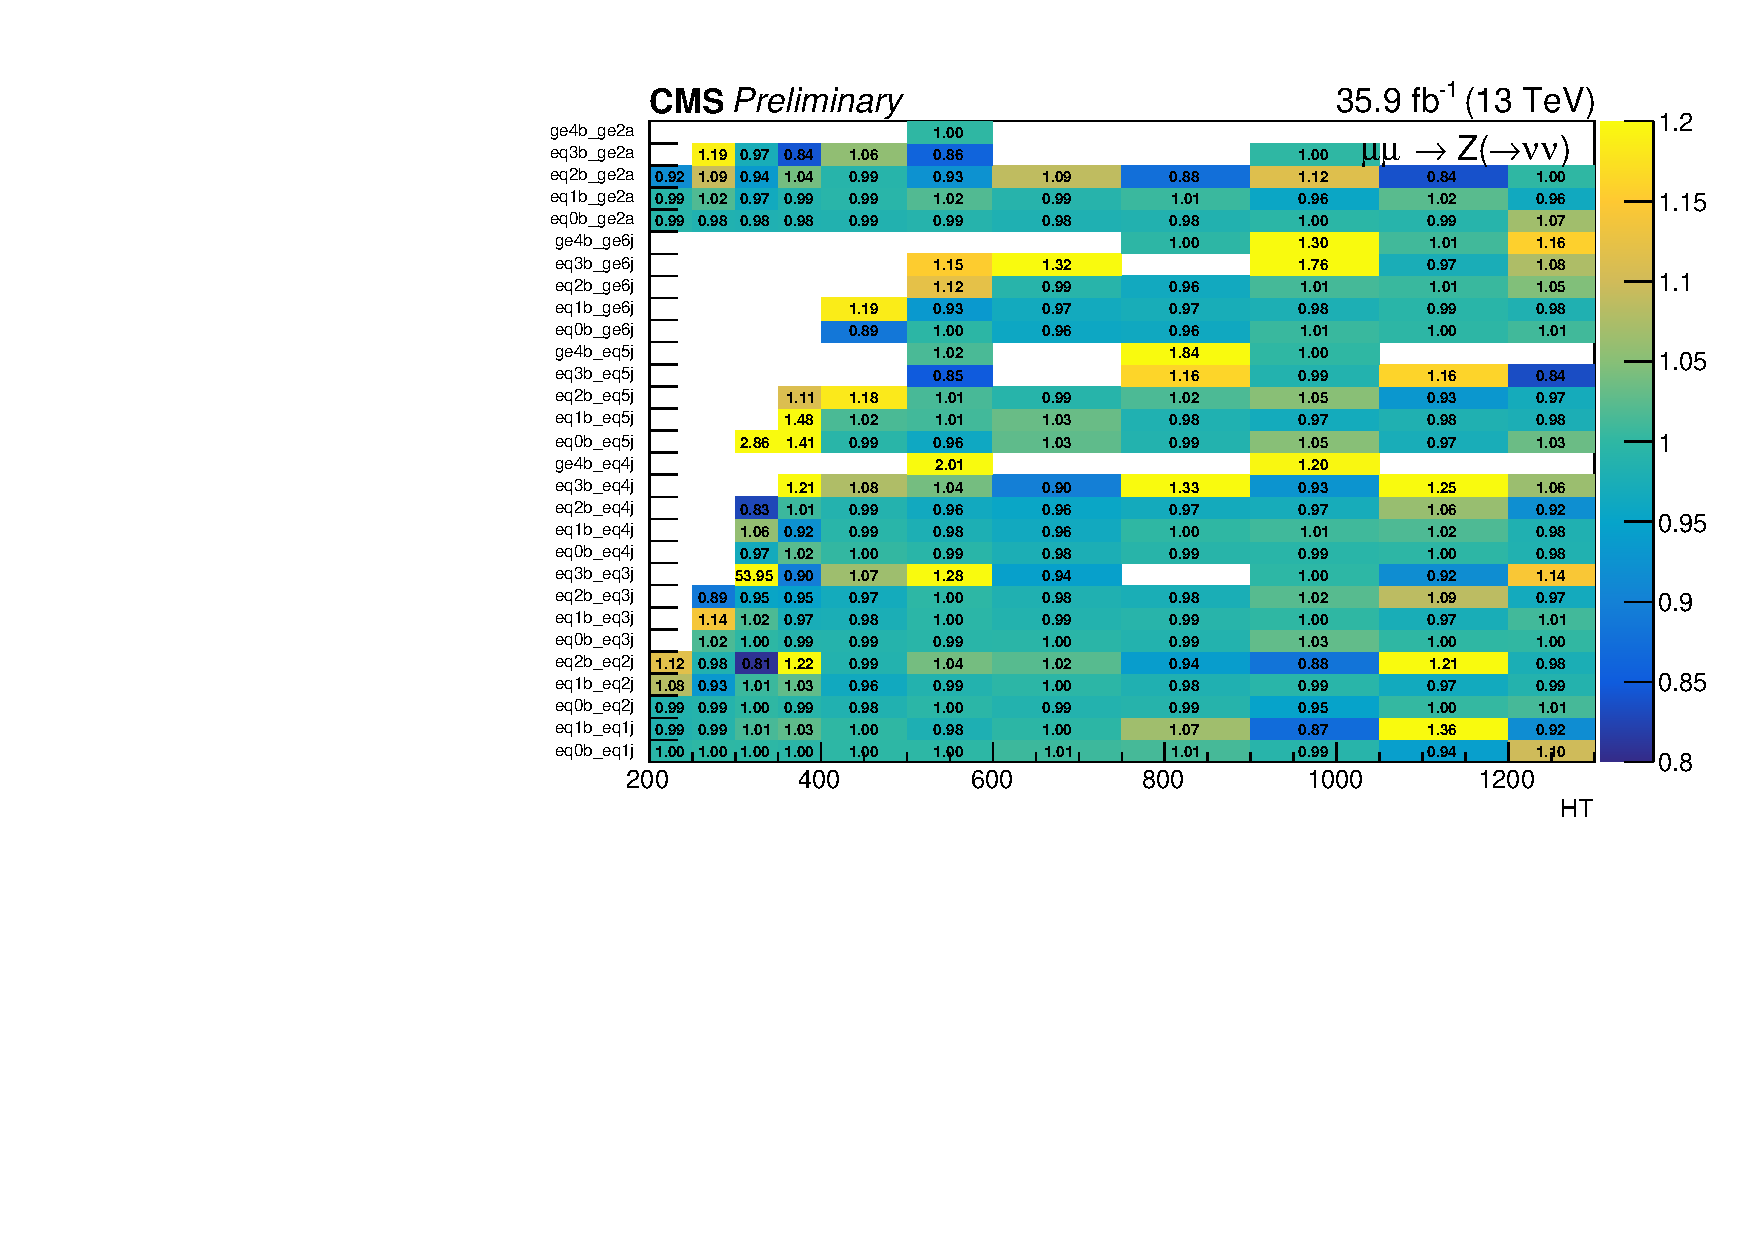
\includegraphics[width=0.5\textwidth]{figures/mcSystematics36p4fb/plots/tfratio_mumu_Zinv_2d_jecDown.pdf}
  }\\
  \subfigure[Up/down variations versus \njet.]{
    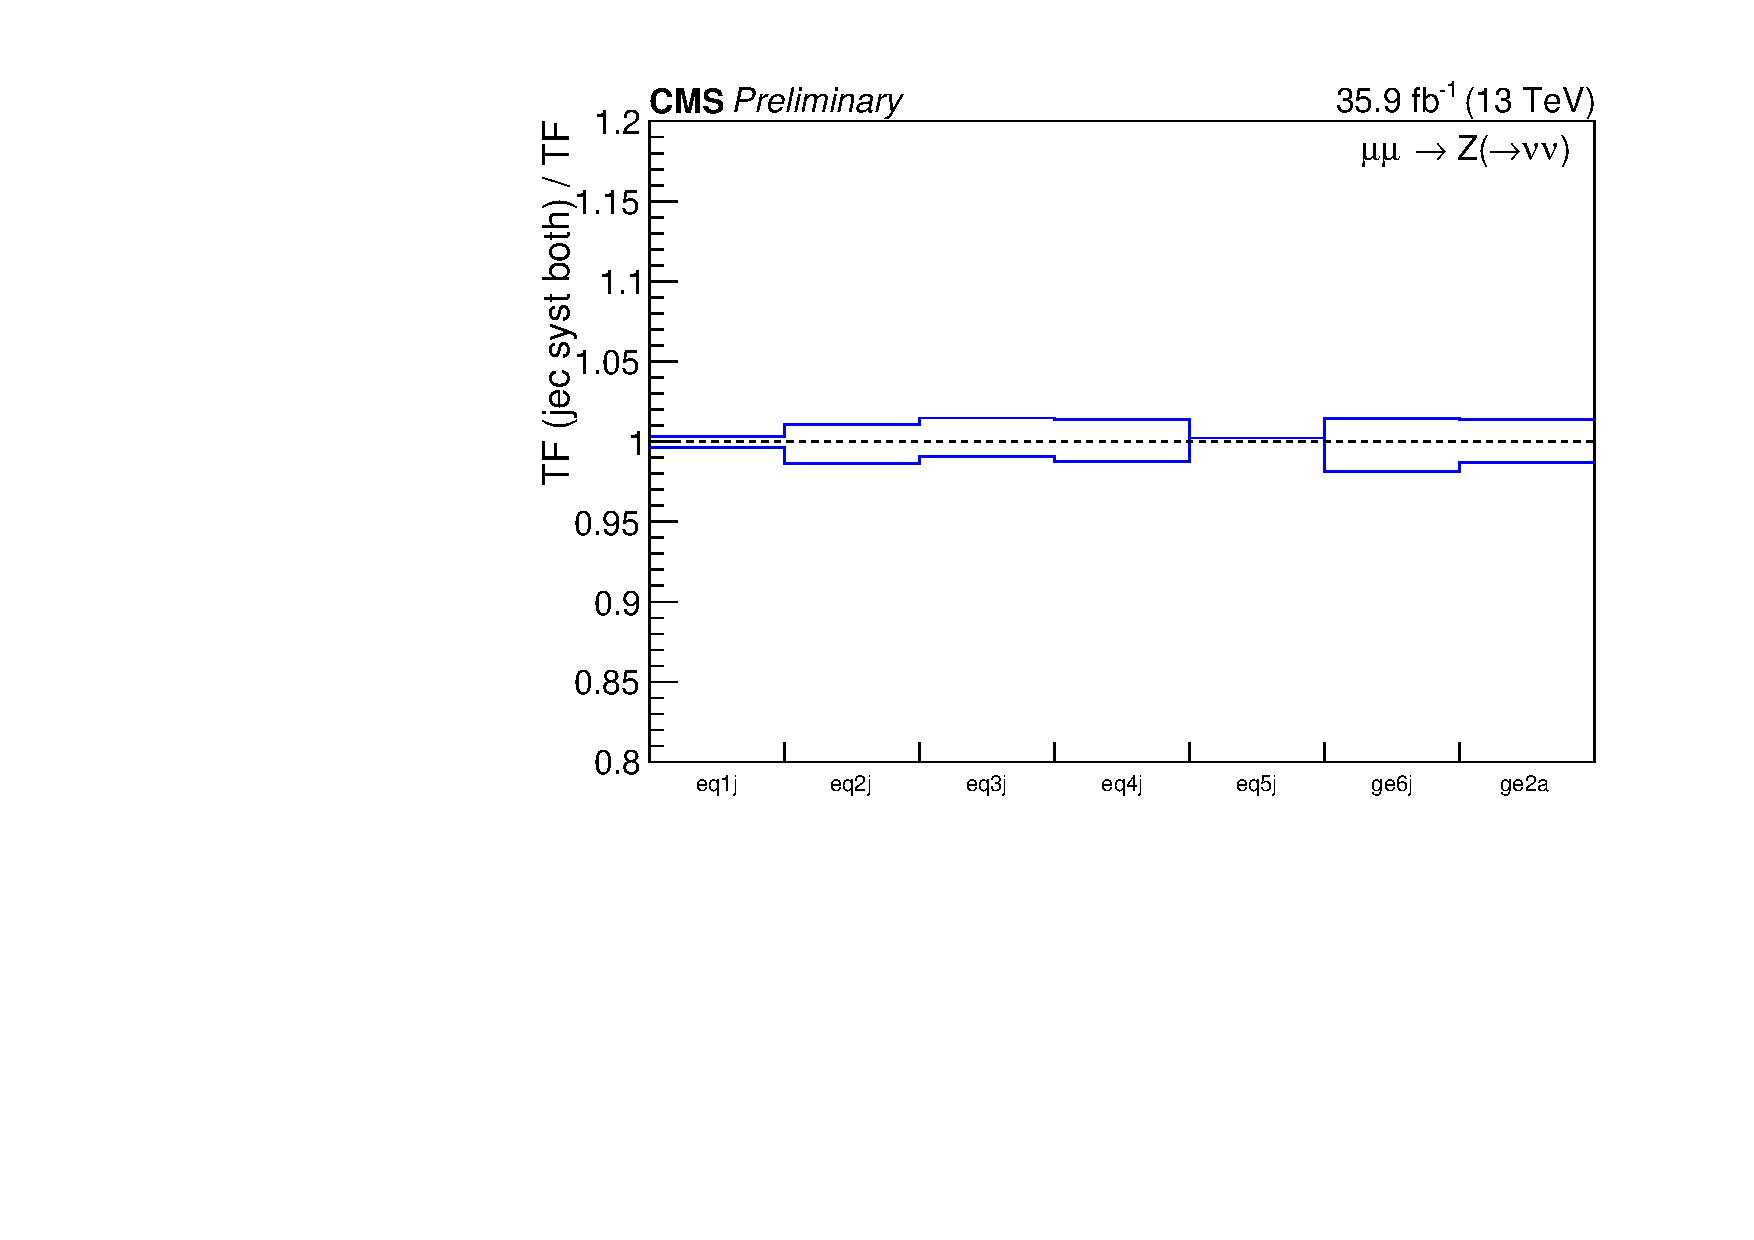
\includegraphics[width=0.5\textwidth]{figures/mcSystematics36p4fb/plots/tfratio_mumu_Zinv_njet_jecUp.pdf}
  } ~
  \subfigure[Up/down variations versus \scalht.]{
    \includegraphics[width=0.5\textwidth]{figures/mcSystematics36p4fb/plots/tfratio_mumu_Zinv_ht_jecUp.pdf}
  } \\
  \subfigure[Up/down variations versus \nb.]{
    \includegraphics[width=0.5\textwidth]{figures/mcSystematics36p4fb/plots/tfratio_mumu_Zinv_bjet_jecUp.pdf}
  } ~
  \subfigure[Up/down variations versus \mht.]{
    \includegraphics[width=0.5\textwidth]{figures/mcSystematics36p4fb/plots/tfratio_mumu_Zinv_ht_jecUp.pdf}
  } \\
  \caption{\label{fig:tfSyst_jec_mumuToZinv} The relative change in the
    ``$\mmj \rightarrow \znunu\ + \textrm{jets}$'' transfer factors from
    simulation due to $\pm1\sigma$ uncertainties in corrections to the
    jet energy scale.  }
\end{figure}

\clearpage
\subsection{B-tagging efficiency and mistag probability}

\begin{figure}[!h]
  \centering
  \subfigure[Up variation versus (\njet,\nb) category and \scalht.]{
    \includegraphics[width=0.5\textwidth]{figures/mcSystematics36p4fb/plots/tfratio_mumu_Zinv_2d_bsfWeightUp.pdf}
  } ~
  \subfigure[Down variation versus (\njet,\nb) category and \scalht.]{
    \includegraphics[width=0.5\textwidth]{figures/mcSystematics36p4fb/plots/tfratio_mumu_Zinv_2d_bsfWeightDown.pdf}
  }\\
  \subfigure[Up/down variations versus \njet.]{
    \includegraphics[width=0.5\textwidth]{figures/mcSystematics36p4fb/plots/tfratio_mumu_Zinv_njet_bsfWeightUp.pdf}
  } ~
  \subfigure[Up/down variations versus \scalht.]{
    \includegraphics[width=0.5\textwidth]{figures/mcSystematics36p4fb/plots/tfratio_mumu_Zinv_ht_bsfWeightUp.pdf}
  } \\
  \subfigure[Up/down variations versus \nb.]{
    \includegraphics[width=0.5\textwidth]{figures/mcSystematics36p4fb/plots/tfratio_mumu_Zinv_bjet_bsfWeightUp.pdf}
  } ~
  \subfigure[Up/down variations versus \mht.]{
    \includegraphics[width=0.5\textwidth]{figures/mcSystematics36p4fb/plots/tfratio_mumu_Zinv_ht_bsfWeightUp.pdf}
  } \\
  \caption{\label{fig:tfSyst_bsf_mumuToZinv} The relative change in the
    ``$\mmj \rightarrow \znunu\ + \textrm{jets}$'' transfer factors from
    simulation due to $\pm1\sigma$ uncertainties in the data/MC scale
    factors associated with b-quark tag efficiency.  }
\end{figure}

\clearpage
\begin{figure}[!h]
  \centering
  \subfigure[Up variation versus (\njet,\nb) category and \scalht.]{
    \includegraphics[width=0.5\textwidth]{figures/mcSystematics36p4fb/plots/tfratio_mumu_Zinv_2d_bsfLightWeightUp.pdf}
  } ~
  \subfigure[Down variation versus (\njet,\nb) category and \scalht.]{
    \includegraphics[width=0.5\textwidth]{figures/mcSystematics36p4fb/plots/tfratio_mumu_Zinv_2d_bsfLightWeightDown.pdf}
  }\\
  \subfigure[Up/down variations versus \njet.]{
    \includegraphics[width=0.5\textwidth]{figures/mcSystematics36p4fb/plots/tfratio_mumu_Zinv_njet_bsfLightWeightUp.pdf}
  } ~
  \subfigure[Up/down variations versus \scalht.]{
    \includegraphics[width=0.5\textwidth]{figures/mcSystematics36p4fb/plots/tfratio_mumu_Zinv_ht_bsfLightWeightUp.pdf}
  } \\
  \subfigure[Up/down variations versus \nb.]{
    \includegraphics[width=0.5\textwidth]{figures/mcSystematics36p4fb/plots/tfratio_mumu_Zinv_bjet_bsfLightWeightUp.pdf}
  } ~
  \subfigure[Up/down variations versus \mht.]{
    \includegraphics[width=0.5\textwidth]{figures/mcSystematics36p4fb/plots/tfratio_mumu_Zinv_ht_bsfLightWeightUp.pdf}
  } \\
  \caption{\label{fig:tfSyst_bsfl_mumuToZinv} The relative change in the
    ``$\mmj \rightarrow \znunu\ + \textrm{jets}$'' transfer factors from
    simulation due to $\pm1\sigma$ uncertainties in the data/MC scale
    factors associated with b-quark mistag probabilities.  }
\end{figure}

\clearpage
\subsection{Extrapolation in \texorpdfstring{\alphat}{AlphaT}}

\begin{figure}[h!]
  \begin{center}
    \includegraphics[width=0.45\textwidth]{figures/closureTests/AlphaT/DoubleMu_alphaTExtrapolation_ht.pdf}~
    \includegraphics[width=0.45\textwidth]{figures/closureTests/AlphaT/DoubleMu_alphaTExtrapolation_nJet.pdf}\\
    \caption{Data-driven closure tests probing the modelling of an
      extrapolation in the \alphat variable with the \mmj sample. The
      level of closure (solid markers) is indicated as a function of
      \scalht (left) and \njet (right). The blue histogram indicates
      the quadrature sum of the magnitude of non-closure and its
      statistical uncertainty. The post-fit closure (open markers) is
      also shown (see text for details).  }
    \label{fig:closure_AlphaT_mumu}
  \end{center} 
\end{figure}

%\begin{figure}[h!]
%  \begin{center}
%    \includegraphics[width=0.45\textwidth]{figures/closureTests/AlphaT/SinglePhoton_alphaTExtrapolation_ht.pdf}~
%    \includegraphics[width=0.45\textwidth]{figures/closureTests/AlphaT/SinglePhoton_alphaTExtrapolation_nJet.pdf}\\ 
%    \caption{As for Fig.~\ref{fig:closure_AlphaT_mu} but probing the
%      modelling of an extrapolation in the \alphat variable with the
%      \gj sample.
%    }
%    \label{fig:closure_AlphaT_phot}
%  \end{center} 
%\end{figure}

%\begin{figure}[h!]
%  \begin{center}
%    \includegraphics[width=0.45\textwidth]{figures/closureTests/AlphaT/AlphaT_Correlated_nuisances.pdf}
%    \caption{The post-fit nuisance parameter values (relative to
%      pre-fit) for the \alphat closure test when implemented as a
%      binned likelihood fit.} 
%    \label{fig:closure_AlphaT_LH_mu}
%  \end{center} 
%\end{figure}

\clearpage
\subsection{Extrapolation in \texorpdfstring{\bdphi}{biased dPhi}}

\begin{figure}[h!]
  \begin{center}
    \includegraphics[width=0.45\textwidth]{figures/closureTests/bDPhi/DoubleMu_bdphiExtrapolation_ht.pdf}~
    \includegraphics[width=0.45\textwidth]{figures/closureTests/bDPhi/DoubleMu_bdphiExtrapolation_nJet.pdf}\\
    \caption{Data-driven closure tests probing the modelling of an
      extrapolation in the \bdphi variable with the \mmj sample. The
      level of closure (solid markers) is indicated as a function of
      \scalht (left) and \njet (right). The blue histogram indicates
      the quadrature sum of the magnitude of non-closure and its
      statistical uncertainty. The post-fit closure (open markers) is
      also shown (see text for details).  }
    \label{fig:closure_bDPhi_mumu}
  \end{center} 
\end{figure}

%\begin{figure}[h!]
%  \begin{center}
%    \includegraphics[width=0.45\textwidth]{figures/closureTests/bDPhi/SinglePhoton_bdphiExtrapolation_ht.pdf}~
%    \includegraphics[width=0.45\textwidth]{figures/closureTests/bDPhi/SinglePhoton_bdphiExtrapolation_nJet.pdf}\\ 
%    \caption{As for Fig.~\ref{fig:closure_bDPhi_mu} but probing the
%      modelling of an extrapolation in the \bdphi variable with the
%      \gj sample.
%    }
%    \label{fig:closure_bDPhi_phot}
%  \end{center} 
%\end{figure}

\clearpage
\subsection{Extrapolation in \texorpdfstring{\alphat}{AlphaT} and
  \texorpdfstring{\bdphi}{biased dPhi}}

\begin{figure}[h!]
  \begin{center}
    \includegraphics[width=0.45\textwidth]{figures/closureTests/AlphaT_bDPhi/DoubleMu_alphaTbdphi_ht.pdf}~
    \includegraphics[width=0.45\textwidth]{figures/closureTests/AlphaT_bDPhi/DoubleMu_alphaTbdphi_nJet.pdf}\\
    \caption{Data-driven closure tests probing the modelling of an
      extrapolation in both \alphat and \bdphi variables, as done in
      the analysis, with the \mmj sample. The level of closure (solid
      markers) is indicated as a function of \scalht (left) and \njet
      (right). The blue histogram indicates the quadrature sum of the
      magnitude of non-closure and its statistical uncertainty. The
      post-fit closure (open markers) is also shown (see text for
      details). \fixme{UPDATE PLOTS WITH CLOSURE FIT!} }
    \label{fig:closure_AlphaT_bDPhi_mumu}
  \end{center} 
\end{figure}

%\begin{figure}[h!]
%  \begin{center}
%    \includegraphics[width=0.45\textwidth]{figures/closureTests/AlphaT/AlphaT_Correlated_nuisances.pdf}
%    \caption{The post-fit nuisance parameter values (relative to
%      pre-fit) for the combined \alphat and \bdphi closure test when
%      implemented as a binned likelihood fit. \fixme{UPDATE PLOT!!!}} 
%    \label{fig:closure_AlphaT_bDPhi_LH_mu}
%  \end{center} 
%\end{figure}

\clearpage
\subsection{The single isolated track veto}

\begin{figure}[h!]
  \begin{center}
    \includegraphics[width=0.45\textwidth]{figures/closureTests/SITV/DoubleMu_Sit_ht.pdf}~
    \includegraphics[width=0.45\textwidth]{figures/closureTests/SITV/DoubleMu_Sit_nJet.pdf}\\
    \caption{Data-driven closure tests that probe the modelling of the
      single isolated track veto. The level of closure (solid markers)
      is indicated as a function of \scalht (left) and \njet
      (right). The blue histogram indicates the quadrature sum of the
      magnitude of non-closure and its statistical uncertainty. }
    \label{fig:closure_SITV_mu}
  \end{center} 
\end{figure}

